%\documentclass[12pt,a4paper]{article} % A4 paper and 11pt font size
\documentclass[12pt]{thesis}  % default square logo 

\usepackage[utf8x]{inputenc}
\usepackage{braket}
\usepackage{amsmath}
\usepackage{bm}
%\usepackage[utf8]{inputenc}
\usepackage{verbatim}
\usepackage{tikz}
%\usepackage{tikz-feynman}
%\usepackage{pgfornament}
\usepackage{pgfplots}
\usepackage{pgffor}
\usepackage[version-1-compatibility, separate-uncertainty=true]{siunitx}
\usepackage{fancyhdr}
\usepackage{lipsum}
%\usepackage{gensymb}
\usepackage{framed}
\usepackage{cancel}
\usepackage{slashed}
\usepackage{hyperref}
\usepackage{pdflscape}
\usepackage{graphicx}
\usepackage{caption}
\usepackage{subcaption}
\usepackage{geometry}
\usepackage{yfonts}
\usepackage{calc}
\usepackage{cite}
\usepackage{caption}
\usepackage{subcaption}
% rotated tables (and figures if necessary)
%\usepackage{fullpage}
\usepackage{graphicx}
\usepackage{rotating}
% Coloured rows in table
\usepackage{color, colortbl}
\usepackage{amssymb}

\usepackage{titlesec, color}
\definecolor{gray75}{gray}{0.75}
\newcommand{\hsp}{\hspace{20pt}}
\titleformat{\chapter}[hang]{\Huge\bfseries}{\thechapter\hsp\textcolor{gray75}{$\lvert$}\hsp}{0pt}{\Huge\bfseries}

%%%%%%%%%%%%%%%CATE'S PREAMBLE BIT (TikZ for Feynman diagrams)%%%%%%%%%%%%%%%%
\usepackage{tikz}
\usetikzlibrary{arrows,shapes}
\usetikzlibrary{trees}
\usetikzlibrary{patterns}
\usetikzlibrary{matrix,arrows} 				% For commutative diagram
											% http://www.felixl.de/commu.pdf
\usetikzlibrary{positioning}				% For "above of=" commands
\usetikzlibrary{calc,through}				% For coordinates
\usetikzlibrary{decorations.pathreplacing}  % For curly braces
% http://www.math.ucla.edu/~getreuer/tikz.html
\usepackage{pgffor}							% For repeating patterns

\usetikzlibrary{decorations.pathmorphing}	% For Feynman Diagrams
\usetikzlibrary{decorations.markings}
\tikzset{
	% >=stealth', %%  Uncomment for more conventional arrows
    vector/.style={decorate, decoration={snake}, draw},
	provector/.style={decorate, decoration={snake,amplitude=2.5pt}, draw},
	antivector/.style={decorate, decoration={snake,amplitude=-2.5pt}, draw},
    fermion/.style={draw=black, postaction={decorate},
        decoration={markings,mark=at position .55 with {\arrow[draw=black]{>}}}},
    fermionbar/.style={draw=black, postaction={decorate},
        decoration={markings,mark=at position .55 with {\arrow[draw=black]{<}}}},
    fermionnoarrow/.style={draw=black},
    gluon/.style={decorate, draw=black,
        decoration={coil,amplitude=4pt, segment length=5pt}},
    scalar/.style={dashed,draw=black, postaction={decorate},
        decoration={markings,mark=at position .55 with {\arrow[draw=black]{>}}}},
    neutrino/.style={dashed,draw=black},
    scalarbar/.style={dashed,draw=black, postaction={decorate},
        decoration={markings,mark=at position .55 with {\arrow[draw=black]{<}}}},
    scalarnoarrow/.style={dashed,draw=black},
    electron/.style={draw=black, postaction={decorate},
        decoration={markings,mark=at position .55 with {\arrow[draw=black]{>}}}},
    bigvector/.style={decorate, decoration={snake,amplitude=4pt}, draw},
    arrow/.style={draw=black, postaction={decorate},
        decoration={markings,mark=at position 1 with {\arrow[draw=black]{>}}}},
}

% TIKZ - for block diagrams, 
% from http://www.texample.net/tikz/examples/control-system-principles/
% \usetikzlibrary{shapes,arrows}
\tikzstyle{block} = [draw, rectangle, 
    minimum height=3em, minimum width=6earticlem]

\tikzset{>=latex}

\tikzset{cross/.style={cross out, draw, minimum size=2*(#1-\pgflinewidth),
			inner sep=0pt, outer sep=0pt}}
			
\tikzset{snake it/.style={decorate, decoration=snake}}

%%%%%%%%%%%%%%END CATE'S PREAMBLE BIT%%%%%%%%%%%%%

%\setlength{\parindent}{2em}
%\setlength{\parskip}{1em}
\newcommand{\goth}[1]{{\Huge\textfrak{#1}}}
\renewcommand{\baselinestretch}{0.9}

\newcommand{\br}{\mathcal{B}}
\newcommand{\tmg}{\tau\to\mu\gamma}
\newcommand{\tlg}{\tau\to\ell\gamma}
\newcommand{\htm}{h\to \tau \mu}
\newcommand{\HRule}{\rule{\linewidth}{0.5mm}}

 \geometry{
 a4paper,
 total={210mm,297mm},
 left=20mm,
 right=20mm,
 top=30mm,
 bottom=30mm,
 }

%----------------------------------------------------------------------------------------
%	TITLE SECTION
%----------------------------------------------------------------------------------------


\title{Lepton flavour violation\\in $\tau$ decays at Belle II }   %note \\[1ex] is a line break in the title

\author{Braden Moore}             %your name
\college{School of Physics}  %your college

%\renewcommand{\submittedtext}{change the default text here if needed}
\degree{Master of Science}     %the degree
\degreedate{28 October 2016}         %the degree date

%end the preamble and start the document
\begin{document}

%this baselineskip gives sufficient line spacing for an examiner to easily
%markup the thesis with comments
\baselineskip=14pt 

%set the number of sectioning levels that get number and appear in the contents
\setcounter{secnumdepth}{3}
\setcounter{tocdepth}{3}

\pagestyle{empty}
\maketitle                  % create a title page from the preamble info

%----------------------------------------------------------------------------------------

\pagestyle{plain}
\begin{romanpages}
\tableofcontents

\chapter*{Abstract}

A study of charged lepton flavour violating $\tau$ decays $\tau\to\mu\gamma$ and $\tau\to e\gamma$ at Belle II was performed over a $\SI{1}{ab^{-1}}$ total luminosity Monte Carlo sample. A $\SI{90}{\percent}$ confidence level upper limit of $\mathcal{B}(\tau\to\mu\gamma)<\num{2.726d-8}$ was found, consistent with previous searches. Precision measusrents of electron modes were found to not be fully supported by the Belle II software at this stage, so no branching fraction was determined for $\tau\to e\gamma$.

\section*{Statement of originality}

Chapters 1 and 2 are an original review of the literature performed by the author, and all experimental work in Chapters 3 - 9 is the author's own unless otherwise stated.

\end{romanpages}


\chapter{Lepton Flavour Violation and the Standard Model}

Lepton flavour violation (LFV) is an exciting field of research at the frontier of particle physics. Searches for LFV probe a wide variety of new physics (NP) scenarios. In most NP models which describe LFV in the $\tau$ sector, the decay modes $\tau\to\ell\gamma$ ($\ell=\mu,e$) have the greatest probability\cite{Paradisi:2016}. It is these modes which we seek to investigate with this analysis.

   \begin{figure}[h]
        \centering
        \begin{subfigure}[b]{0.475\textwidth}
            \centering
            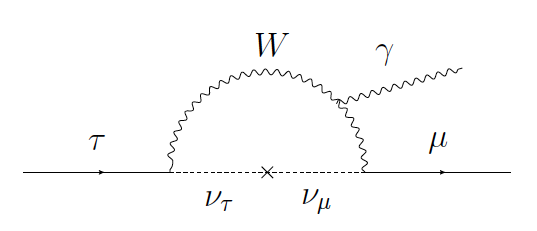
\includegraphics[width=\textwidth]{images/tauMG-feynman.png}
            \caption[]%
            {{\small}}   
            \label{fig:tauMG feynman} 
        \end{subfigure}
        \hfill
        \begin{subfigure}[b]{0.475\textwidth}  
            \centering 
            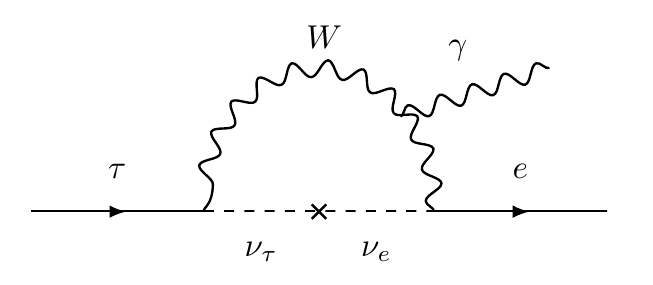
\includegraphics[width=\textwidth]{images/tauEG-feynman.png}
            \caption[]%
            {{\small}}    
            \label{fig:tauEG feynman}
        \end{subfigure}
        \caption{Feynman diagrams for (a) $\tau\to\mu\gamma$ and (b) $\tau\to e\gamma$ proceeding through SM processes.}
    \end{figure}

LFV necessarily requires generation mixing between leptons to occur. Though this is prohibited in the Standard Model, the discovery of neutrino oscillations proves that flavour mixing does occur in our universe --- that is, flavour is not conserved. Neutrino oscillations occur due to the finite but very small mass of the neutrinos. However, the Standard Model cannot explain how neutrinos have this mass. There must be new physics coupling to leptons which faciliates the mass generation of neutrinos, and this new physics may induce charged LFV.

In the SM modified to include massive neutrinos, LFV processes can occur through processes shown in Figures~\ref{fig:tauMG feynman} and~\ref{fig:tauEG feynman}. However, these Feynman diagrams are greatly suppressed and are proportional to the Glashow-Iliopoulo-Maiani (GIM) factor, given as $\left(\frac{m_\nu}{M_W}\right)^4$. As neutrino mass is very small ($\mathcal{O}(\SI{0.3}{eV})$) we expect any LFV effects in the SM to be negligible. With these operators the branching ratio for $\tmg$ is $\sim 10^{-40}$ \cite{Passemar:2015}, and similarly small for $\tau\to e\gamma$. With such little SM background, observation of an LFV process of the type $\tlg$ would be an unambiguous signature of NP.

\begin{equation}
\mathcal{B}(\tau\to\ell\gamma)=\frac{3\alpha}{32\pi}\lvert U^{\star}_{\tau i} U_{\mu i}\frac{\Delta^2_{3i}}{m_W^2}\rvert^2
\leq 10^{-53}\sim 10^{-49}
\end{equation}


\section{Other LFV}

In many NP models, LFV is not limited to just $\tlg$ decays. There have been searches for other LFV modes, such as $\mu\to e \gamma$, and $\tau\to 3\ell$. Current limits on the branching fractions are given in Figure \ref{tab:current lfv bounds} below \cite{Paradisi:2016}.

\begin{table}[h]
\centering
\label{my-label}
\begin{tabular}{lll}
\hline
\textbf{LFV process} & \textbf{Present bound} & \textbf{Future sensitivity} \\ \hline
$\mu\to e\gamma$ & \num{5.7e-13} & $\approx\num{6e-14}$ \\
$\mu\to 3e$ & \num{1.0e-12} & $\approx\num{e-16}$ \\
$\tau\to e\gamma$ & \num{3.3e-9} & $\sim\num{e-8} - \num{e-9}$ \\
$\tau\to\mu\gamma$ & \num{4.4e-9} & $\sim\num{e-8} - \num{e-9}$ \\
$\tau\to 3e$ & \num{2.7e-8} & $\sim\num{e-9} - \num{e-10}$ \\
$\tau\to 3\mu$ & \num{2.1e-8} & $\sim\num{e-9} - \num{e-10}$ \\
\hline
\end{tabular}
\caption{Current experimental limits on various LFV processes}
\label{tab:current lfv bounds}
\end{table}

Moving into future sensitivities accessible from experiments such as Belle II, we see that the upper limits of branching fractions for $\tlg$ decays could be improved by $1-2$ orders of magnitude.

\section{Hints of LFV beyond the Standard Model}

Motivations behind the search for LFV come from both theoretical and experimental results. The primary experimental motivation is the existence of neutrino mass, though anomalous results such as the $\htm$ excess observed at CMS in 2015 also hint at LFV beyond the Standard Model. On the theoretical side, LFV is predicted in a variety of NP models. In fact, many models which introduce mechanisms to generate neutrino mass also allow LFV in other sectors of non-negligible order. We shall discuss these motivations below.

\subsection{Neutrino mixing}

The discovery that flavour mixing can occur in the neutrino sector \cite{Fukuda:1998}\cite{McGregor:2002} proves that neutrinos have mass. Both the concept of massive neutrinos, and by extension the mechanisms which generate neutrino mass, are not predicted or explained by the SM. This tells us that the lepton sector is not fully understood.

There are many NP models which introduce mechanisms to give neutrinos mass. These include SUSY, seesaw models, and many others. In introducing these mechanisms, many of these models inadvertently introduce LFV. As a particular example, a Type-II seesaw model posits a scalar triplet of Higgs-like particles \cite{Passemar:2015}. This triplet comprises a doubly-charged Higgs, a singly-charged Higgs, and a neutral Higgs. As show in Figure X below, lepton-flavour violating processes could proceed via leptons coupling to these scalars.


\begin{figure}[h]
\centering
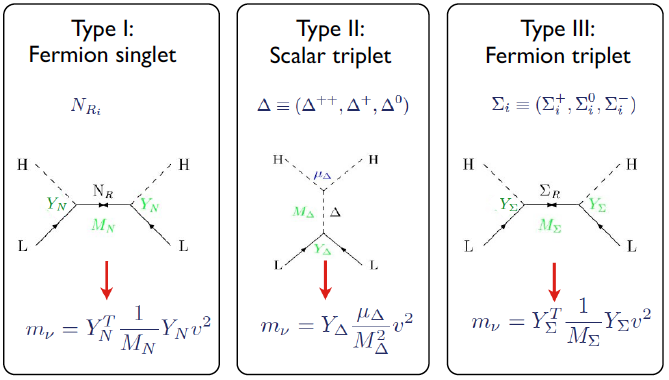
\includegraphics[width=0.7\textwidth]{images/seesaw.png}
\caption[]%
{{\small New particles introduced in seesaw models (Passemar, 2015)}}
\label{}
\end{figure}

\begin{figure}[h]
\centering
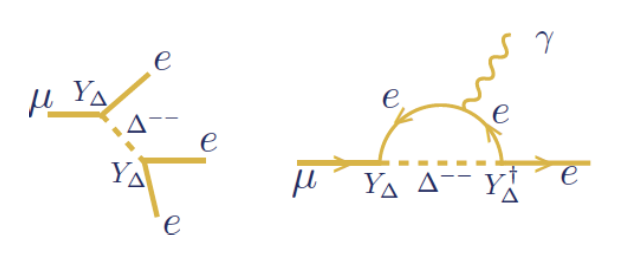
\includegraphics[width=0.5\textwidth]{images/seesaw-lfv-modes.png}
\caption[]%
{{\small Scalars introduced in Type-II seesaw models mediating LFV decays (Passemar, 2015). $\Delta^{--}$ are doubly-charged scalars.}}
\label{}
\end{figure}

\subsection{$\htm$ excess}

Hints of LFV come in the form of experimental results which are not consistent with the SM. One such ``anomaly’’ was the $\htm$ excess observed at the LHC. In 2015, CMS found a $2.4\sigma$ excess in the branching fraction of $\htm$ \cite{Khachatryan:2015}. This process is lepton flavour violating, so in the SM its branching fraction is expected to be consistent with zero. However it was determined

\begin{equation}
\br(h\to \tau \mu) = (0.84^{+0.39}_{-0.37})\%
\end{equation}

Also in 2015 was a similar search performed by ATLAS \cite{Aad:2015}, in which an excess of $1.2\sigma$ was found in the $\htm$ decay. 

\begin{equation}
B(\htm) = (0.77 \pm 0.66)\%
\end{equation}

Though this $1.2\sigma$ result is less indicative of NP, it still provides hints as to where NP could occur. These results indicate possible new physics in the Higgs sector. Several models, including Two-Higgs Doublet Models (2HDM), introduce new Higgs-like particles; these particles can couple with leptons to allow lepton flavour violating processes \cite{Harnik:2012}. In fact, LFV can occur naturally in any model with more than one Higgs doublet.

\begin{figure}[h]
\centering
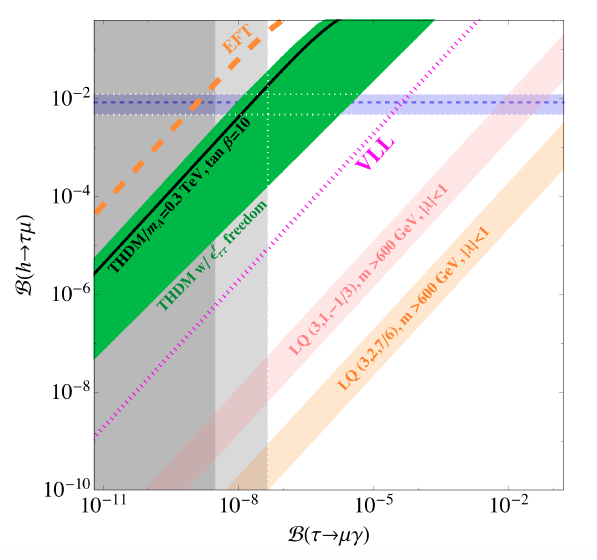
\includegraphics[width=0.7\textwidth]{images/h-vs-tau.png}
\caption{Correlation between $\br(\htm)$ and $\br(\tmg)$ in various NP scenarios (Dorsner et al., 2015)}
\label{}
\end{figure}

The present experimental result for $\br(\htm)$ is shown in the horizontal blue band. Current and future projections for $\br(\tmg)$ experimental sensitivity are represented by vertical light and dark gray bands. We note that certain 2HDM models predict a branching fraction for $\br(\tmg)$, consistent with the CMS results, at sensitivities which could be observed by Belle II. It is important to note that the Higgs sector could contribute to LFV in NP scenarios, and that both theory and experimental limits on other LFV processes such as $\htm$ all interweave with limits on $\tlg$ branching fractions to provide information on NP, even just through reducing the available phase space for certain models \cite{Dorsner:2015}.

\begin{figure}[h]
\centering
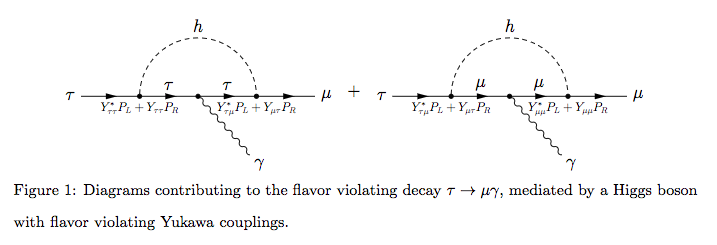
\includegraphics[width=0.9\textwidth]{images/higgs-lfv-modes.png}
\caption[]%
{{\small Diagrams contributing to $\tmg$ decay, mediated by a Higgs boson (Harnick et al., 2012).}}
\label{}
\end{figure}



As seen in Figure above, new Higgs particles can mediate LFV processes and allow for measurable amounts of LFV beyond the Standard Model \cite{Dorsner:2015}.


\subsection{Models predicting $\tlg$}

As mentioned previously, LFV in the $\tau$ sector is introduced in many NP scenarios as a consequence of generating neutrino mass (and hence facilitating neutrino mixing). Branching fractions of the modes $\tlg$ are highly calculable - there is little theoretical uncertainty.

\begin{table}[h]
\centering
\begin{tabular}{cc}
\hline \textbf{model} & $\mathcal{B}(\tau\to\mu\gamma)$ \\ \hline
mSUGRA + seesaw & \num{d-7} \\
SUSY + SO(10) & \num{d-8} \\
SM + seesaw & \num{d-9} \\
Non-Universal Z' & \num{d-9} \\
SUSY + Higgs & \num{d-10} \\ \hline
\end{tabular}
\caption[]%
{{\small Upper limits of branching fractions from $\tmg$, predicted by models of new physics beyond the SM (various sources)\cite{Ohshima:2007}.}}
\label{tab:bounds by NP}
\end{table}

Figure above lists a few NP models with their predictions of $\br(\tmg)$. We see that the phase space of some of these models has already been ruled out with our current experimental limits on LFV branching fractions.


\section{Past searches for $\tlg$}

The most recent searches for $\tlg$ were undertaken at Belle (2007) and Babar (2010), for both $\ell=\mu,e$ modes. These experiments both used $e^+ e^-$ colliders to generate physics events. A signal of the form $e^+ e^-\to \tau^+ \tau^-$, with one $\tau$ (signal-side) decaying $\tau\to \ell \gamma$ and the other $\tau$ (tag-side) decaying generically, with the requirement that the tag-side track is not $\ell$.


\subsection{Belle searches}


   \begin{figure}[h]
        \centering
        \begin{subfigure}[b]{0.475\textwidth}
            \centering
            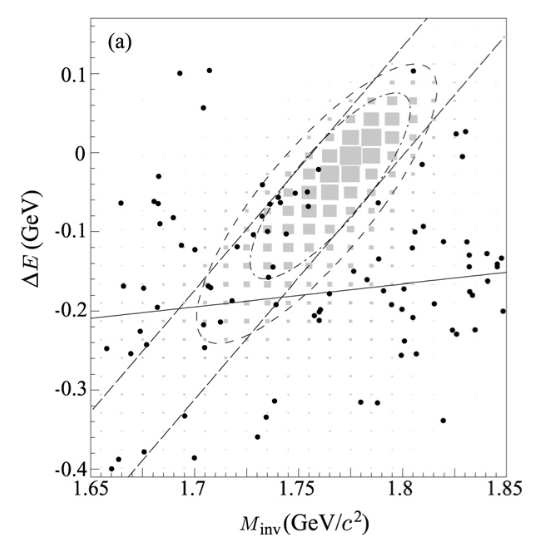
\includegraphics[width=\textwidth]{images/belle-search-tauMG-signal-region.png}
            \caption[]%
            {{\small}}    
            \label{fig:Belle search tauMG signal region}
        \end{subfigure}
        \hfill
        \begin{subfigure}[b]{0.475\textwidth}  
            \centering 
            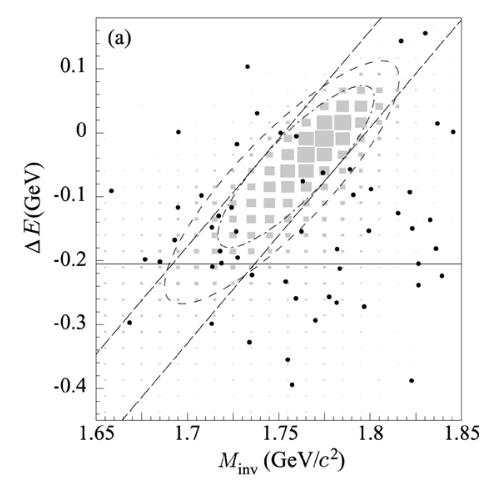
\includegraphics[width=\textwidth]{images/belle-search-tauEG-signal-region.png}
            \caption[]%
            {{\small}}    
            \label{fig:Belle search tauEG signal region}
        \end{subfigure}
        \caption{$M_{\text{inv}}$-$\Delta E$ distribution in the search for (a) $\tau\to\mu\gamma$ and (b) $\tau\to e\gamma$ at Belle over a $\SI{535}{fb^{-1}}$ data set. $M_{\text{inv}}$ is the reconstructed mass of the $\tau$ from these processes, $\Delta E$ is the energy difference between this reconstructed $\tau$ and half center-of-mass frame beam energy. Dots are the data and shaded boxes indicate the signal MC. The dashed ellipse shows the $3\sigma$ region and the dot-dashed ellipse is the $2\sigma$ signal region.}
    \end{figure}


The Belle detector records events from an asymmetric $e^+ e^-$ collider with electron (positron) energy of $\SI{8}{GeV}$ ($\SI{3.5}{GeV}$). A detailed discussion of the detector can be found at Ref. \cite{Abashian:2000cg}. A search for $\tau\to\ell\gamma$ was performed over $\SI{535}{fb^{-1}}$ and set constraints \cite{Hayasaka:2007vc} on $\tlg$ branching fractions as

\begin{align*}
\br(\tmg)&<\num{4.5d-8},\\
\br(\tau\to e \gamma)&<\num{1.2d-7}.
\end{align*}

Events were selected by applying selection criteria to twenty event-related variables including momentas and energies; the signal regions for $\tau\to\mu\gamma$ and $\tau\to e\gamma$ after selection are shown in Figures~\ref{fig:Belle search tauMG signal region} and~\ref{fig:Belle search tauEG signal region} respectively. Signal efficiencies, defined as the ratio of generated events to events remaining, in the $2\sigma$ regions were $\epsilon_{\tau\to\mu\gamma}=\SI{5.07}{\percent}$ and $\epsilon_{\tau\to e\gamma}=\SI{2.99}{\percent}$. For the muon mode, dominant backgrounds (non-signal events also produced in $e^+ e^-$ collisions) were found to be $e^+ e^- \to \tau^+ \tau^-$ events with the decay $\tau^{\pm}\to\mu^{\pm}\nu_{\mu}\nu_{\tau}$ or $\tau^{\pm}\to\pi^{\pm}\nu_{\tau}$, and radiative mu-pair processes $e^+ e^- \to \mu^+ \mu^-$. Background sources in the electron mode were found to be radiative Bhabha $e^+ e^- \to e^+ e^- \gamma$ and radiative tau-pair processes $e^+ e^- \to \tau^+ \tau^- \gamma$. 

\subsection{Babar searches}

   \begin{figure}[h]
        \centering
        \begin{subfigure}[b]{0.475\textwidth}
            \centering
            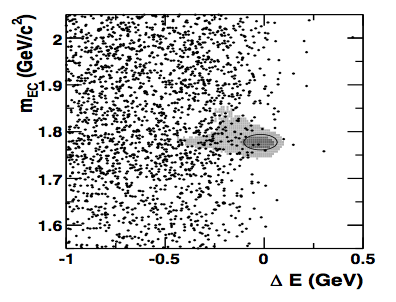
\includegraphics[width=\textwidth]{images/babar-search-tauMG-signal-region.png}
            \caption[Network2]%
            {{\small}}    
        \end{subfigure}
        \hfill
        \begin{subfigure}[b]{0.475\textwidth}  
            \centering 
            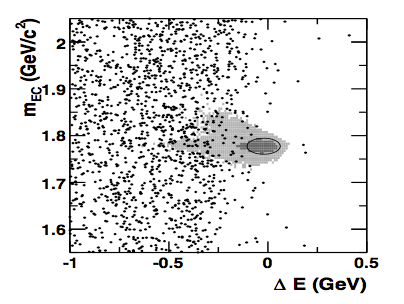
\includegraphics[width=\textwidth]{images/babar-search-tauEG-signal-region.png}
            \caption[]%
            {{\small}}    
        \end{subfigure}
        \caption{$M_{\text{bc}}$-$\Delta E$ distribution in the search for (a) $\tau\to\mu\gamma$ and (b) $\tau\to e\gamma$ at Babar over a $\SI{515.5}{fb^{-1}}$ data set. $M_{\text{bc}}$ is the beam-constrained mass of the $\tau$ from these processes, $\Delta E$ is the energy difference between this reconstructed $\tau$ and half center-of-mass frame beam energy. Data are shown as dots and contours containing \num{90}{\percent} (\num{50}{\percent}) of signal MC events are shown as light- (dark-) shaded regions.}
        \label{fig:babar signal region}
    \end{figure}


Similar to Belle, the Babar detector records events from an asymmetric $e^+e^-$ collider, with electron (positron) energy of $\SI{9}{GeV}$ ($\SI{3.1}{GeV}$). A detailed discussion of the detector can be found at Ref. \cite{Aubert:2001}. The most recent search for $\tlg$ was performed in 2010 by the Babar Collaboration \cite{Aubert:2009ag}, over a $\SI{515.5}{fb^{-1}}$ dataset, setting constraints on $\tlg$ branching fractions as

\begin{align*}
\br(\tmg)&<\num{4.4d-8},\\
\br(\tau\to e \gamma)&<\num{3.3d-8}.
\end{align*}




\section{The role of this analysis}

Collection of data at Belle II is scheduled to begin in 2017. A physics program has been designed for the experiment, detailing specific decays to investigate and areas of particle physics to probe. It is important before data collection begins to perform sensitivity studies on these decay processes, to find areas in which the analysis performs better or worse than expected. In some cases we may find that background rejection is greater than previously modelled due to, for example, good performance in particle identification by the detector. It is also important if areas for improvement are found, such as beam background degrading analysis performance. Finding areas for improvement during the development stage informs future development, including tracking and reconstruction software and hardware-based beam background mitigation techniques, and leads to more optimal conditions for physics events to be investigated.


This analysis is the first $\tau$ physics study for Belle II. Some key points studied are muon and electron track reconstruction and the effects of beam background on reconstructed events. Information on these areas of event analysis is not only useful for $\tau\to\ell\gamma$ searches at Belle II --- the physics program for the experiment includes a range of $\tau$ decay processes (see Table~\ref{tab:current lfv bounds}) of which many require muon and electron track reconstruction. Low-multiplicity events require XXXXXX, so XXXXXX.

\begin{table}[h]
\centering
\label{my-label}
\begin{tabular}{lll}
\hline \textbf{LFV process} & \textbf{Present bound} & \textbf{Future sensitivity} \\ \hline
$\tau\to e\gamma$ & \num{3.3e-9} & $\sim\num{e-8} - \num{e-9}$ \\
$\tau\to\mu\gamma$ & \num{4.4e-9} & $\sim\num{e-8} - \num{e-9}$ \\
$\tau^{\pm}\to e^{\pm} e^{\mp} e^{\pm}$ & \num{2.7e-8} & $\sim\num{e-9} - \num{e-10}$ \\
$\tau^{\pm}\to \mu^{\pm} \mu^{\mp} \mu^{\pm}$ & \num{2.1e-8} & $\sim\num{e-9} - \num{e-10}$ \\
\hline
\end{tabular}
\caption{Current experimental limits on various LFV processes}
\label{tab:current lfv bounds}
\end{table}

Results from this analysis will be published in the Belle II physics book, which is currently being compiled by members across all working groups in the collaboration. The book will provide a resource to inform a range of physics and detector activity across the entire Belle II experiment. This study will provide the basis for future $\tau$ LFV studies at Belle II, and serves to validate the projected increase in sensitivity for $\tau\to\ell\gamma$ branching fractions from Belle to Belle II.

%-------------------------------------------------------------------

\chapter{The Belle and Belle II detectors}

Located in Tsukuba, Japan, the KEKB particle collider was used for the Belle experiment from 1999 to 2010 and collided high energy electrons and positrons of $\SI{8}{GeV}$ and $\SI{3.5}{GeV}$ respectively. This experiment made important discoveries on the flavour structure of elementary particles, notably in the quark section where CP symmetry violation was discovered. Efforts by the Belle collaboration culminated in the 2008 Nobel Prize awarded to Makoto Kobayashi and Toshihide Maskawa for their theory of CP violation\cite{NobelPrize}. Over its lifetime, the Belle detector collected a total time-integrated luminosity of $\SI{1}{ab^{-1}}$, corresponding to \num{919000000} tau-pair events. An upgrade to the KEKB collider known as SuperKEKB is expected to be complete by 2017 as part of the Belle II experiment.

\begin{figure}[h]
\centering
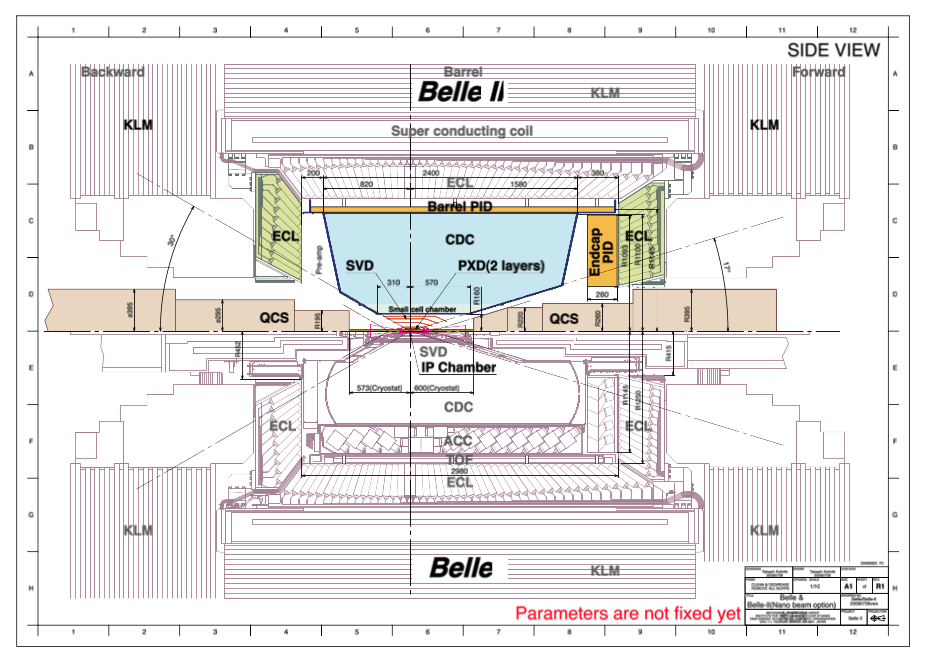
\includegraphics[width=0.8\linewidth]{images/super-kekb-side-view.png}
\caption[]%
{{\small Super-KEKB detector design, side-view.}}
\label{fig:superKEKB}
\end{figure}

Over the course of the experiment, it is projected that Belle II will collect a total time-integrated luminosity of $\SI{50}{ab^{-1}}$. This is a much larger data sample than the $\SI{1}{ab^{-1}}$ collected at Belle. Electron-positron beam energies differ from those used at Belle, with high-energy-ring (HER) electron beam energy of $\SI{7}{GeV}$ and low-energy-ring (LER) positron beam energy  of $\SI{4}{GeV}$. Design luminosity in the detector is increased by 40 over Belle; this increases background incidence rate on the detector by a factor of 20, while physics event rate is expected to be 50 times higher than at Belle.

Key components of the detector are the vertex detector (VXD), the central drift chamber (CDC), the electromagnetic calorimeter (ECL), the time-of-propagation/aerogel ring-imaging Cerenkov detector (TOP/ARICH), and the $K_L$/$\mu$ detector (KLM). Many of these will be upgraded in Belle II to provide better performance; in some cases the full reconstruction software is rewritten even when the hardware is not upgraded.

Coordinates in the detector, such as polar angles and positions along the $z$-axis, are often referred to in the paper, so we shall define them here. The positive $z$-axis runs from the interaction point parallel to the electron beam trajectory; polar angle is the azimuthal angle from the $z$-axis. The detector is rotationally symmetric around the $z$-axis; rotation angles are not discussed in this analysis. The angular acceptable of the detector is from $17^{\circ}$ (forward) to $150^{\circ}$ (backward) --- particles with a polar angle within the angular acceptance will be recorded by the detector. 

The role of detector components in event reconstruction is discussed in Section~\ref{sec:reconstruction process}.

%-------------------------------------------------------------------

\section{Vertex Detector}

Determing the decay vertices of particles --- that is, the point inside the detector which the decay occurs --- was performed at Belle by the Silicon Vertex Detector (SVD2), comprising four layers of double-sided silicon detectors (DSSDs). By the end of its lifetime SVD2 the innermost layer had an average occupancy of \num{10}{\percent}, defined as the fraction of channels hit in each triggered event. This level of occupancy leads to worsened track resolution and reconstruction.

With beam luminosity at Belle II projected to increase by factor 20 over Belle, the greater rate of events due to beam-related backgrounds would worsen SVD2 occupancy and degrade detector performance.  As such the vertexing detector received a redesign moving to Belle II, with a focus on reducing occupancy. This is achieved by the introduction of a two-layer Pixel Detector (PXD) replacing the the DSSDs closest to beam interaction point, and a four-layer Silicon Vertex Detector (SVD) beyond the PXD. Vertexing is important in track counting as it allows the interaction point to be reconstructed.

\subsection{Pixel Detector}

The PXD at Belle II has a far larger number of channels than DSSDs --- 3.072 million pixels in the inner layer, and 4.608 million pixels in the outer layer. This affords a much smaller occupancy even with higher event rate. Pixel layers are located at $\SI{14}{mm}$ and $\SI{22}{mm}$ from the beampipe.


\subsection{Silicon Vertex Detector}

Along with the PXD and the CDC, the SVD is used to measure decay vertices and to extrapolate tracks from charged particles. Track data from the CDC is used in association with SVD data to extrapolate tracks back to the PXD with high efficiency. The SVD comprises four layers of DSSDs at increasing radius from the interaction point: 38, 80, 115, and $\SI{140}{mm}$. As the layers have a larger radius than at Belle, a greater cross-sectional area is covered by the DSSDs, and the quality of reconstruction of charged tracks is improved.

\begin{figure}[h]
\centering
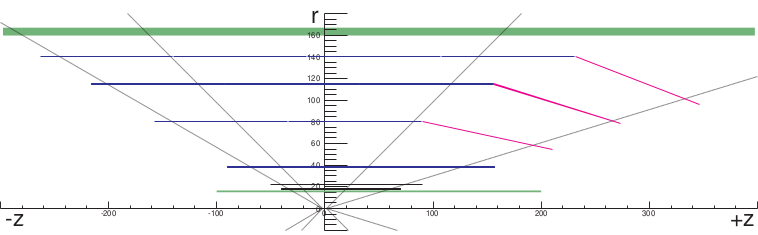
\includegraphics[width=0.8\linewidth]{images/svd.png}
\caption[]%
{{\small Configuration of the four SVD layers (blue), and the two PXD layers (black). Slanted sensors (pink) are used in the forward regions of the outer SVD layers to greatly reduce amount of DSSDs required to cover angular acceptance.}}
\label{fig:svd}
\end{figure} 

%-------------------------------------------------------------------

\section{Central Drift Chamber}

The CDC serves as the primary tracking device of the Belle II detector -- it can precisely determine the momenta of charged tracks passing through, and, with vertex and impact parameter information from the PXD and SVD, facilitates efficient reconstruction of these particle tracks. Particle identification is also assisted by the CDC, with precise $dE/dx$ measurements for charged particles being good indicators of particle species.

The CDC comprises of many cells filled with neutral gas inside a $\SI{1.5}{T}$ magnetic field. The cells are occupied by ``sense wires''; charged particles passing through the CDC cause ionisation of the neutral gas, with the ionised particles colliding with the sense wires.
 
The Belle II upgrade will reduce cell size and increase the volume of the CDC, shifting the inner radius from $\SI{77}{mm}$ to $\SI{160}{mm}$ and extending the outer radius from $\SI{880}{mm}$ to $\SI{1130}{mm}$. Cell sizes are reduced to operate at high event rates with background levels increased from Belle. The number of sense wires is increased from \num{8400} to \num{14336}. A visual representation of this upgrade is shown in Figure~\ref{fig:cdc}.

\begin{figure}[h]
\centering
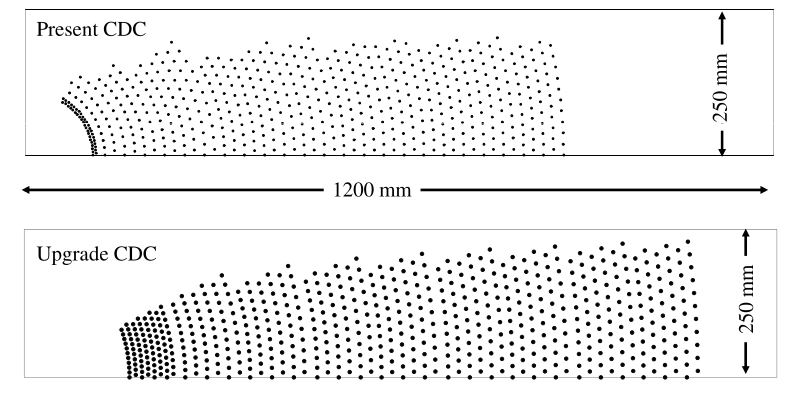
\includegraphics[width=0.7\linewidth]{images/cdc.png}
\caption[]%
{{\small A comparison of the central drift chambers for Belle (top) and Belle II (bottom). The upgraded CDC has a larger volume and greater number of sense wires.}}
\label{fig:cdc}
\end{figure} 


%-------------------------------------------------------------------


\section{Electromagnetic Calorimeter}

The ECL consists of two distinct sections within the detector - a $\SI{3}{m}$ long barrel section with inner radius of $\SI{1.25}{m}$, and annular endcaps located $\SI{1.96}{m}$ forward from the interaction point (IP) along the $z$-axis and $\SI{1.02}{m}$ backwards from the IP along the $z$-axis. At Belle, the barrel section contained 6624 CsI(Tl) scintillator crystals of truncated pyramid shape and average size $6\times 6\times 30\si{cm^3}$ (cross-section multiplied by crystal depth); the endcaps consisted of 2112 CsI(Tl) crystals, with a total of 8736 crystals in the ECL. 

Two main tasks of the ECL are the precise detection of photons and their energy and position within the detector, and identification of electrons. Photons and electrons incident on the barrel and end-cap crystals deposit energy and cause scintillation of the crystals recorded by the detector.

Electronics and event-readout for the ECL will be improved for Belle II, and the end–cap scintillator crystals will be replaced with pure CsI crystals, which have a faster event response and and more radiation-tolerant. Upgrades to the ECL will considerably improve photon energy resolution. Pile-up of unimportant events will also be greatly reduced. Since we are required to reconstruct a signal photon, this improved photon resolution allows for better analysis of $\tau\to\ell\gamma$ modes at Belle II.

%-------------------------------------------------------------------

\section{Time-Of-Propagation/Aerogel Ring Imaging Cerenkov Detector}

Particle identification across all the entire angular acceptance of Belle II is important for effective reconstruction and analysis of a range of physics events. The TOP detector located in the barrel region, and ARICH located in the end-caps allow for improved $K/\pi$ separation over most of their momentum spectrum; limited discriminating power between low momentum pions, muons and electrons is possible in the end-caps.

%-------------------------------------------------------------------

\section{$K_{L}$/muon detector}

The outermost detector component at Belle II is the KLM, used in $K_{L}$ and muon detection. Most electrons and photons generated in a collision do not reach the KLM --- the remaining particles are often muons or charged hadrons ($\pi^\pm$ or $K^\pm$). The KLM exists outside the magnetic field of the detector and consists of alternating sandwich of iron plates of thickness $\SI{4.7}{cm}$, and active detector elements. As with the ECL, the KLM has barrel and end-cap components.

At Belle the active detector elements were glass-electrode resistive plate chambers (RPC). These elements have worsened efficiency under high background fluxes due to their long dead time; at Belle II the end-cap and innermost barrel RPCs have been replaced with scintillators.

We can discriminate charged hadrons such as pions from muons by penetration depth in the KLM. Pions reaching the KLM interact strongly with the hadronic material in the iron plates and produce hadronic showers detected in the ECL or KLM. In doing so the pions lose a lot of energy, and so only shallow penetrate the KLM. Muons do not interact hadronically and so can and can be identified by their long penetration depth. These particles often travel along nearly straight lines through the KLM and exit the detector. High momentum charged pions can appear as `fake' muons in the KLM --- these particles can penetrate the KLM deeply before they are slowed due to hadronic interactions.



%-------------------------------------------------------------------

\section{Particle identification}
\label{sec:PID}

\subsection{Charged particle identification}

Particle tracks in the detector can be identified by a combination of discriminants, such as  dE/dx measured by the CDC and shower shape in the ECL. Probability density functions (PDFs) for these discriminants are known for a range of possible particles, including e, $\mu$, $\pi$ and $K$. Based on each PDF, likelihood probabilities can be calculated then combined to produce a final likelihood variable. This is known as the likelihood ratio $\mathcal{L}_{\mu}$ (in this case a muon likelihood ratio), with range 0 to 1. For an example track, the greater $\mathcal{L}_{\mu}$ is the more probable that track is a muon.

Electron candidates are identified using electron likelihood ratio $\mathcal{L}_e$, which is based on dE/dx information from the CDC, the ratio of energy energy in the ECL and the charged track momentum measured by the SVD and CDC, shower shape at the ECL, matching between positions of a cluster at the ECL and charged track position extrapolated to the ECL, and time-of-flight as measured by the TOF. Identification of muons uses $\mathcal{L}_{\mu}$, which is based on the difference between penetration depth of the track in the KLM as calculated from particle momentum and the measured depth. Kaon and pion candidates are identified using $\mathcal{L}_{K}$ and $\mathcal{L}_{\pi}$ respectively, which are based on the dE/dx measurement from the CDC, and TOP/ARICH measurements \cite{BelleII:tech-design-report}.

Particle identification at Belle II uses particle identification (PID) values for candidate tracks. PID values are constructed from the difference in log likelihood between two particle hypotheses, as
\begin{equation}
\mathcal{L}(\alpha : \beta) = \frac{1}{e^{\ln \mathcal{L}_{\alpha}-\ln\mathcal{L}_{\beta}}}
\end{equation}
where $\alpha$ and $\beta$ are two different particle types. $\mathcal{L}(\alpha : \beta)$ is greater than $0.5$ for charged tracks more likely to be of type $\alpha$ than of $\beta$, and similarly for $\mathcal{L}(\alpha : \beta)$ less than 0.5. Muon PID is defined as $\mu\text{-PID}=\mathcal{L}(\mu:\pi)$, electron PID is defined as $e\text{-PID}=\mathcal{L}(e:\mu)$, while for pions we define $\pi\text{-PID}=\mathcal{L}(\pi:K)$, and similarly for kaons $K\text{-PID}=\mathcal{L}(K:\pi)$.

 \begin{figure}
        \centering
        \begin{subfigure}[b]{0.475\textwidth}
            \centering
            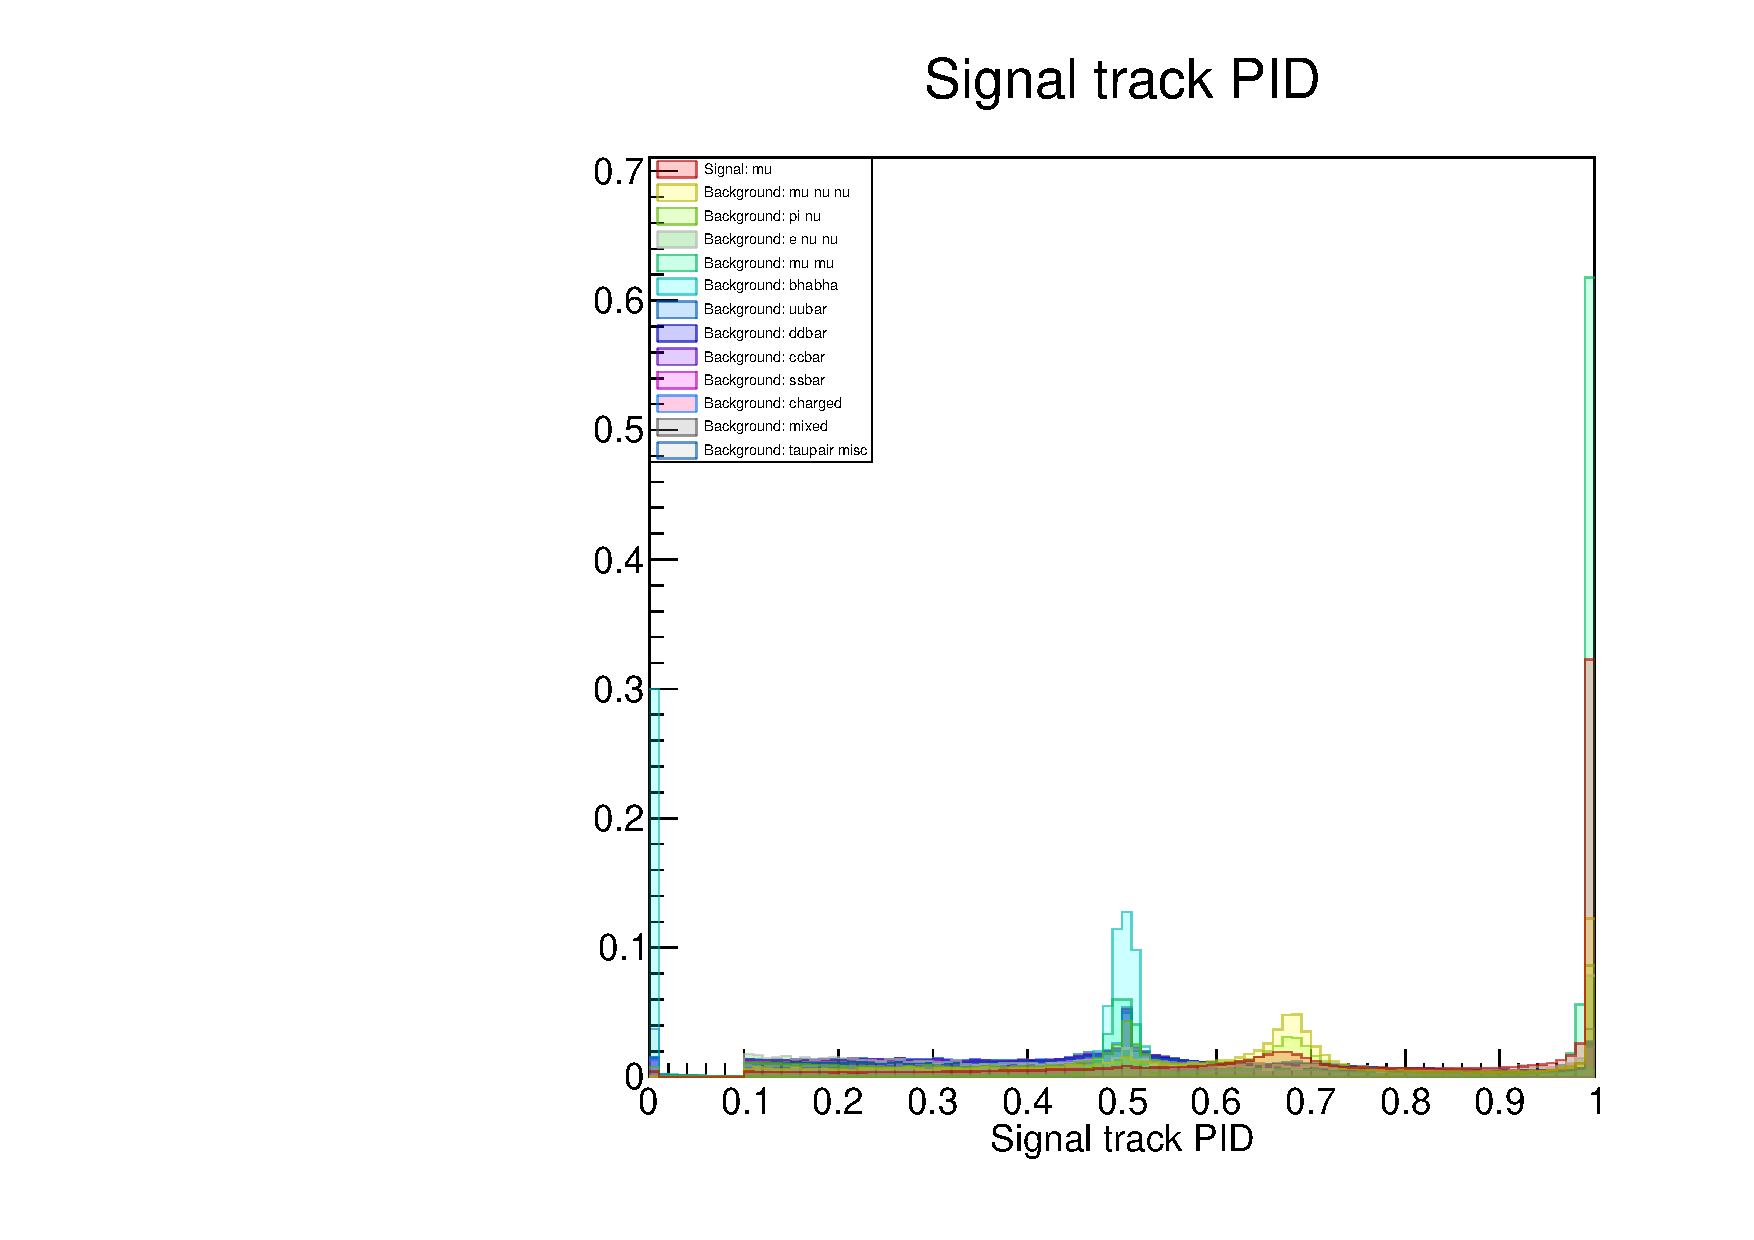
\includegraphics[width=\textwidth]{images/tauMG-sigPIDmu.pdf}
            \caption[]%
            {{\small $\mu$-PID}}    
            \label{fig:tauMG sigPIDmu}
        \end{subfigure}
        \hfill
        \begin{subfigure}[b]{0.475\textwidth}  
            \centering 
            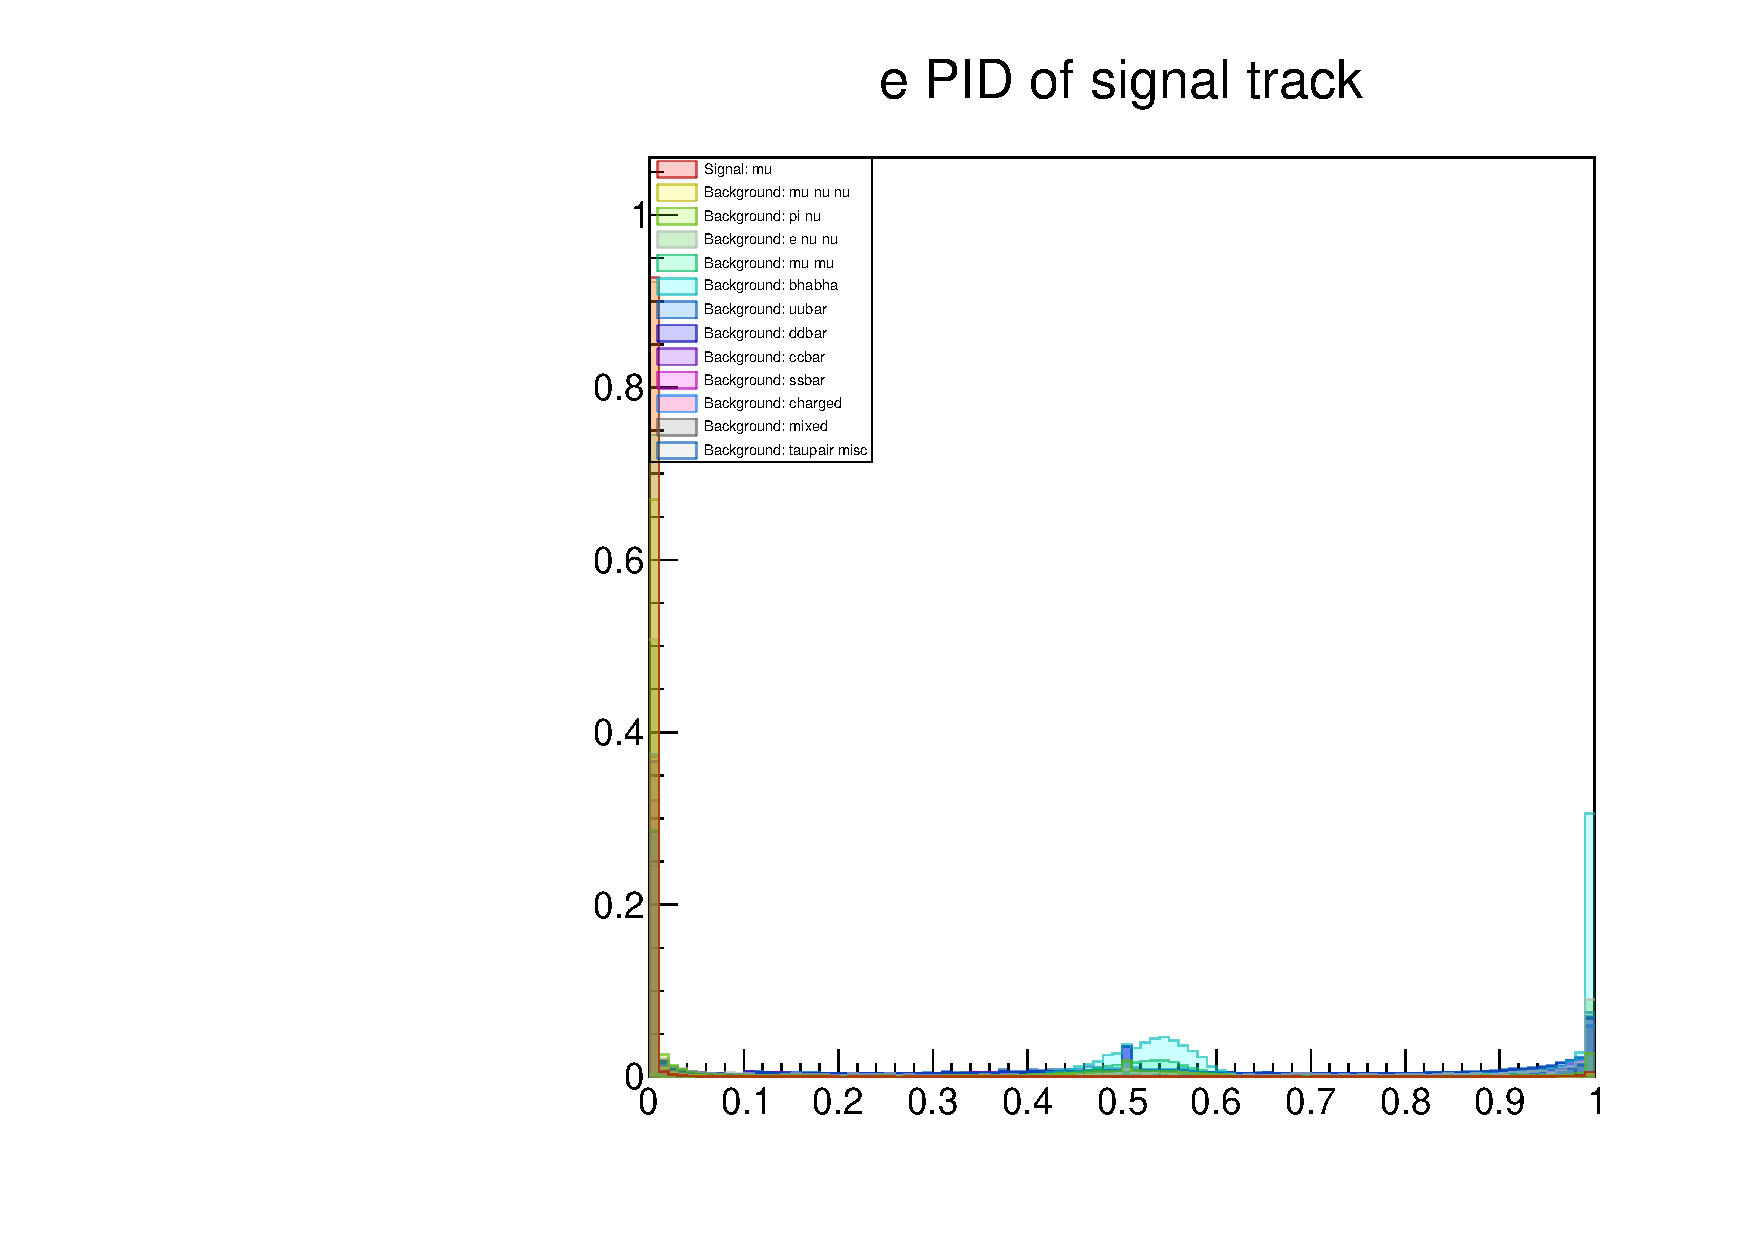
\includegraphics[width=\textwidth]{images/tauMG-sigPIDe.pdf}
            \caption[]%
            {{\small $e$-PID}}    
            \label{fig:tauMG sigPIDe}
        \end{subfigure}
        \vskip\baselineskip
        \begin{subfigure}[b]{0.475\textwidth}   
            \centering 
            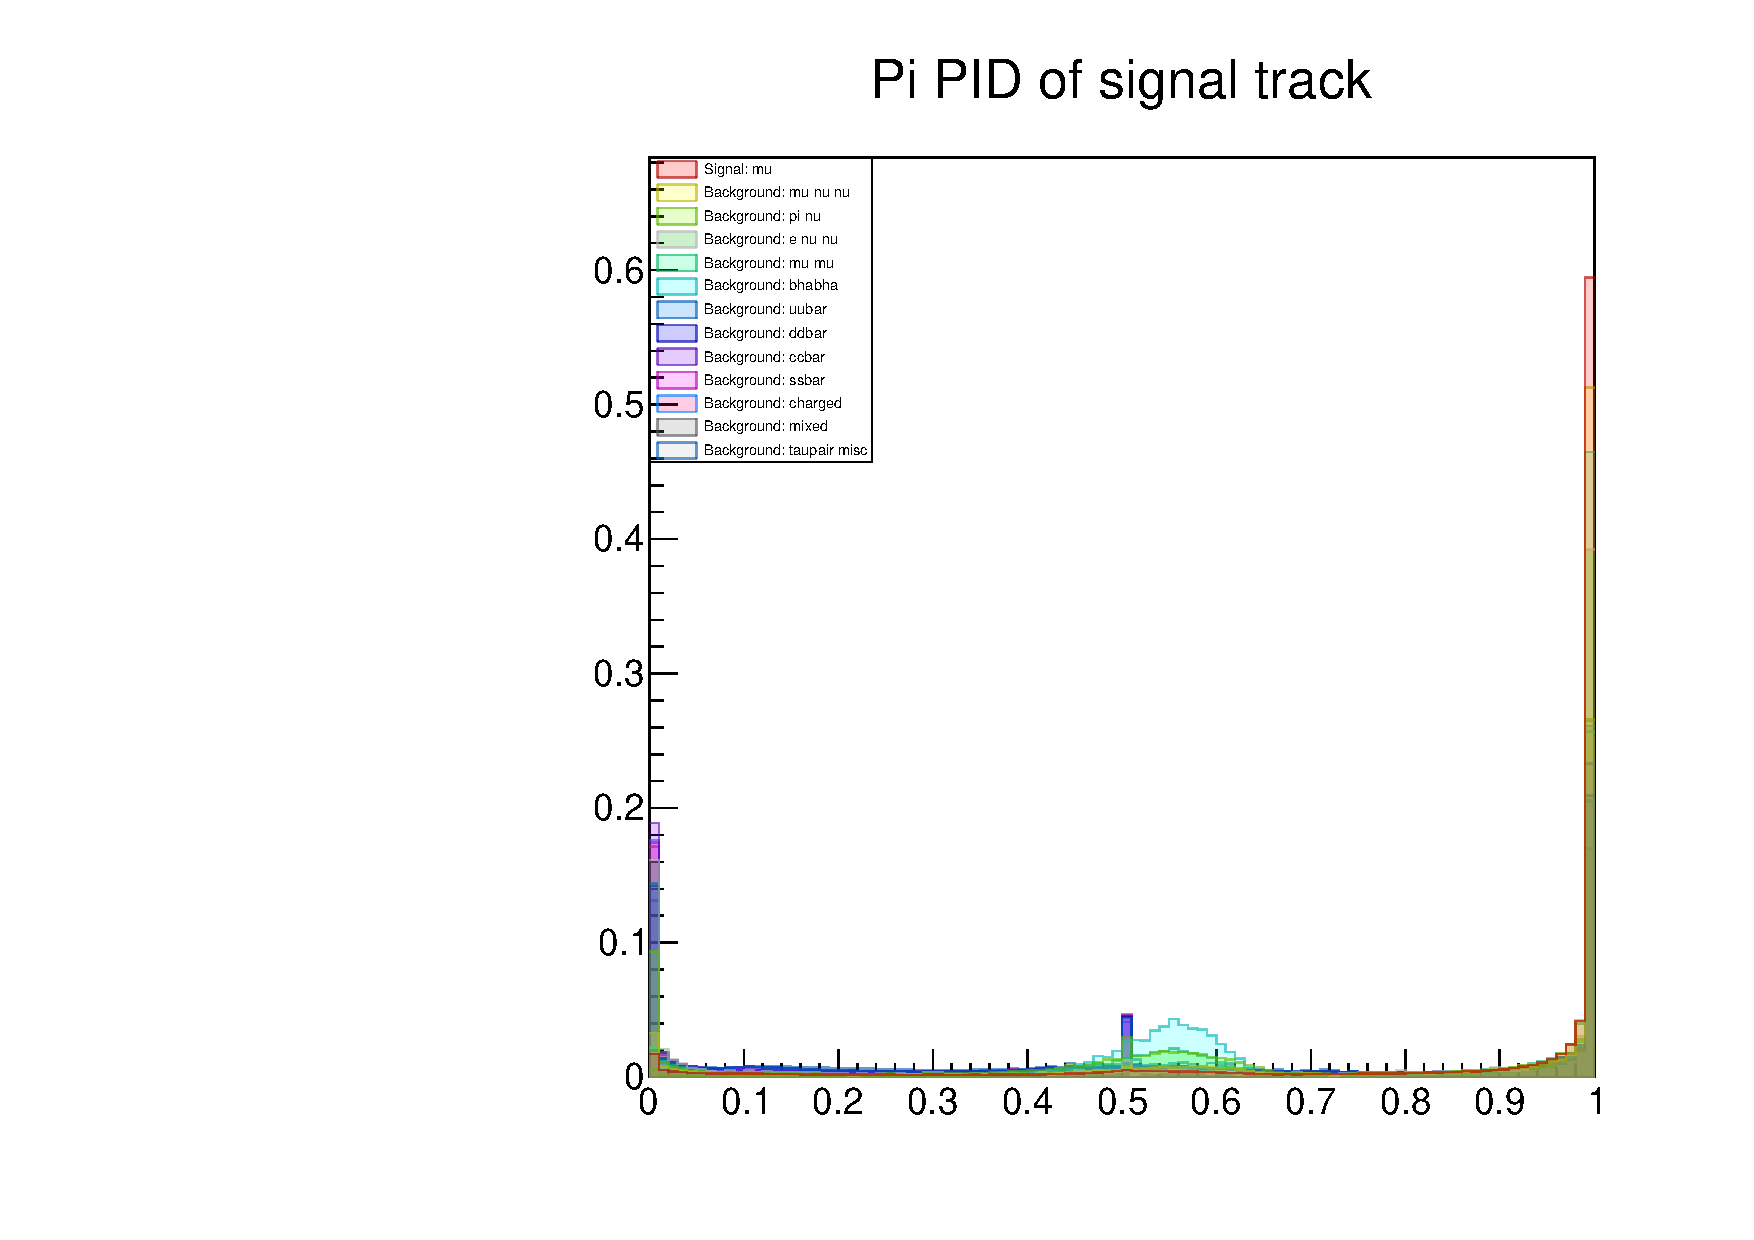
\includegraphics[width=\textwidth]{images/tauMG-sigPIDpi.pdf}
            \caption[]%
            {{\small $\pi$-PID}}    
            \label{fig:tauMG sigPIDpi}
        \end{subfigure}
        \hfill
        \begin{subfigure}[b]{0.475\textwidth}   
            \centering 
            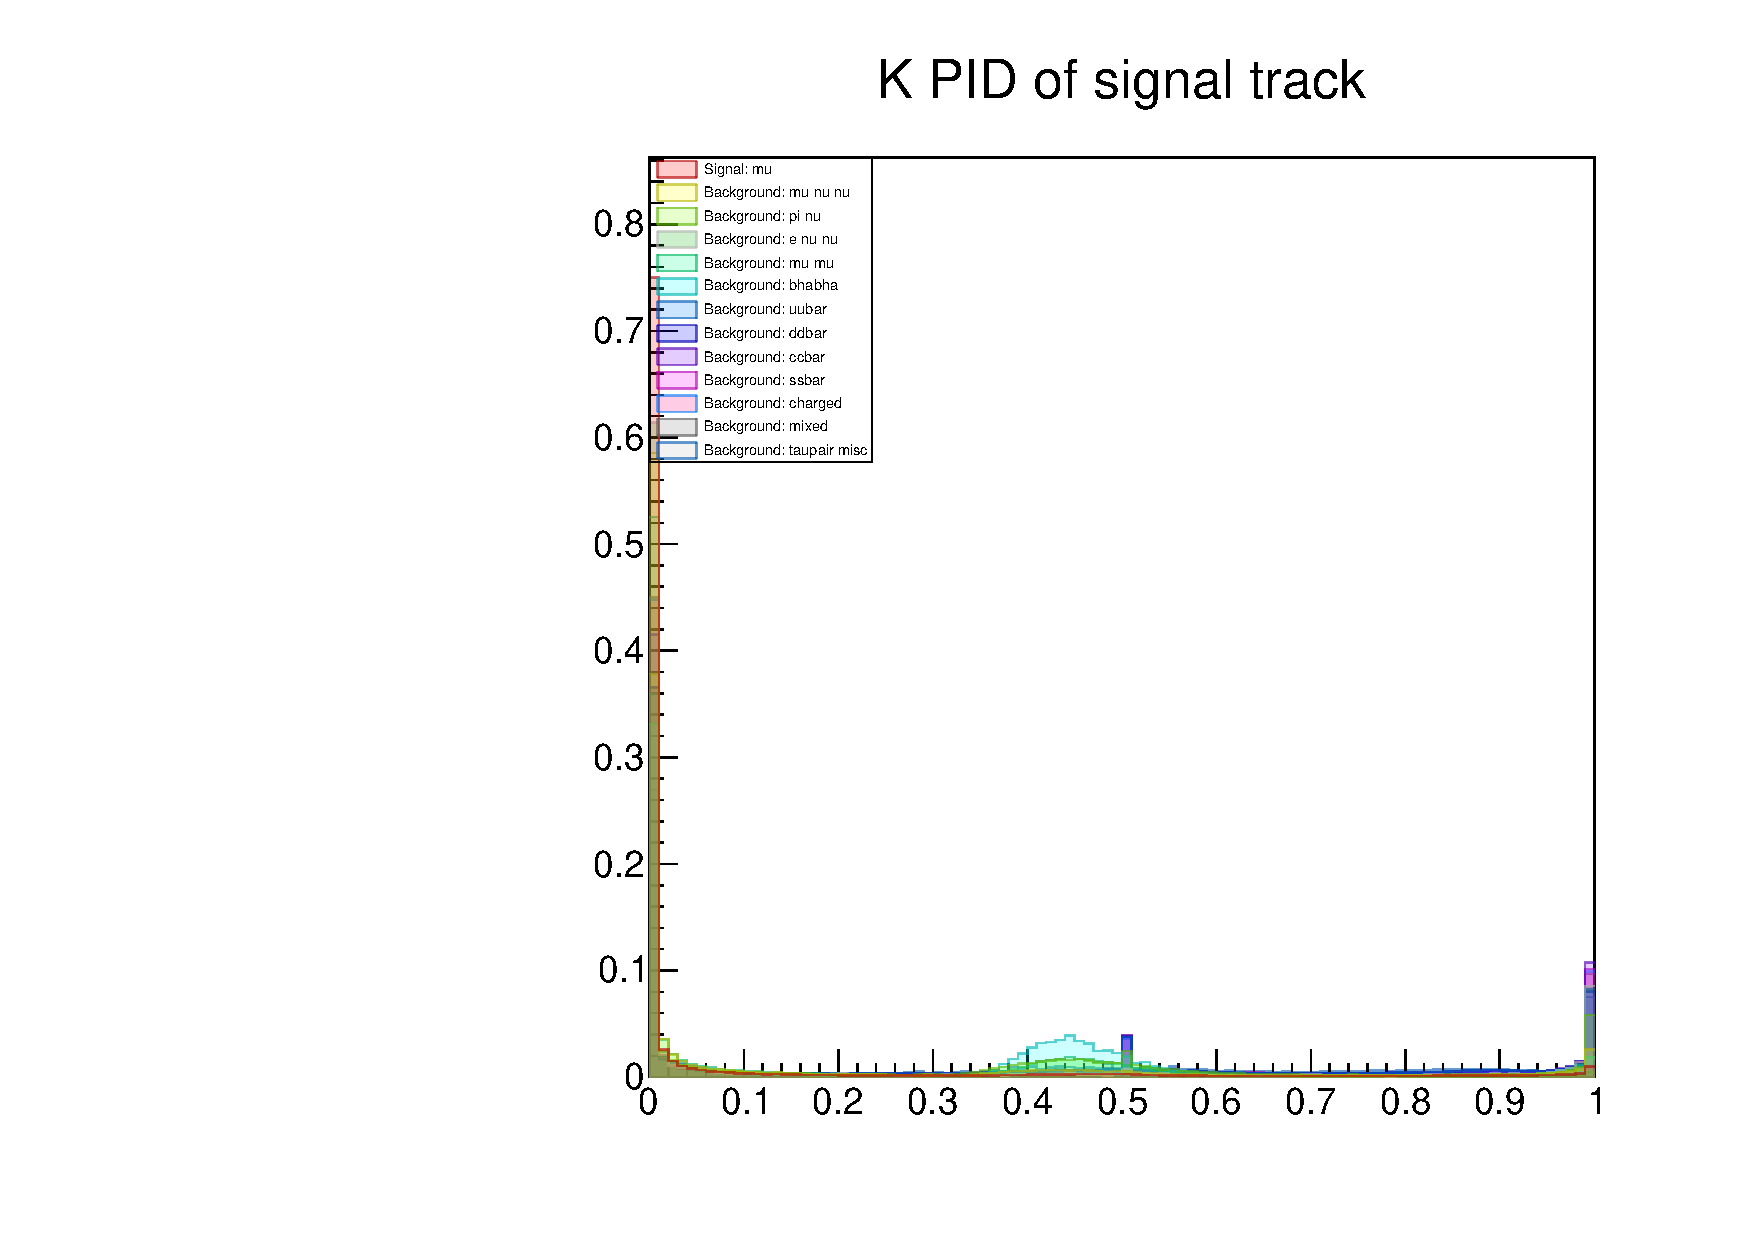
\includegraphics[width=\textwidth]{images/tauMG-sigPIDk.pdf}
            \caption[]%
            {{\small $K$-PID}}    
            \label{fig:tauMG sigPIDk}
        \end{subfigure}
        \caption[]
        {\small PID values for signal track.} 
        \label{fig:tauMG sigPIDk}
    \end{figure}


\begin{figure}
\centering
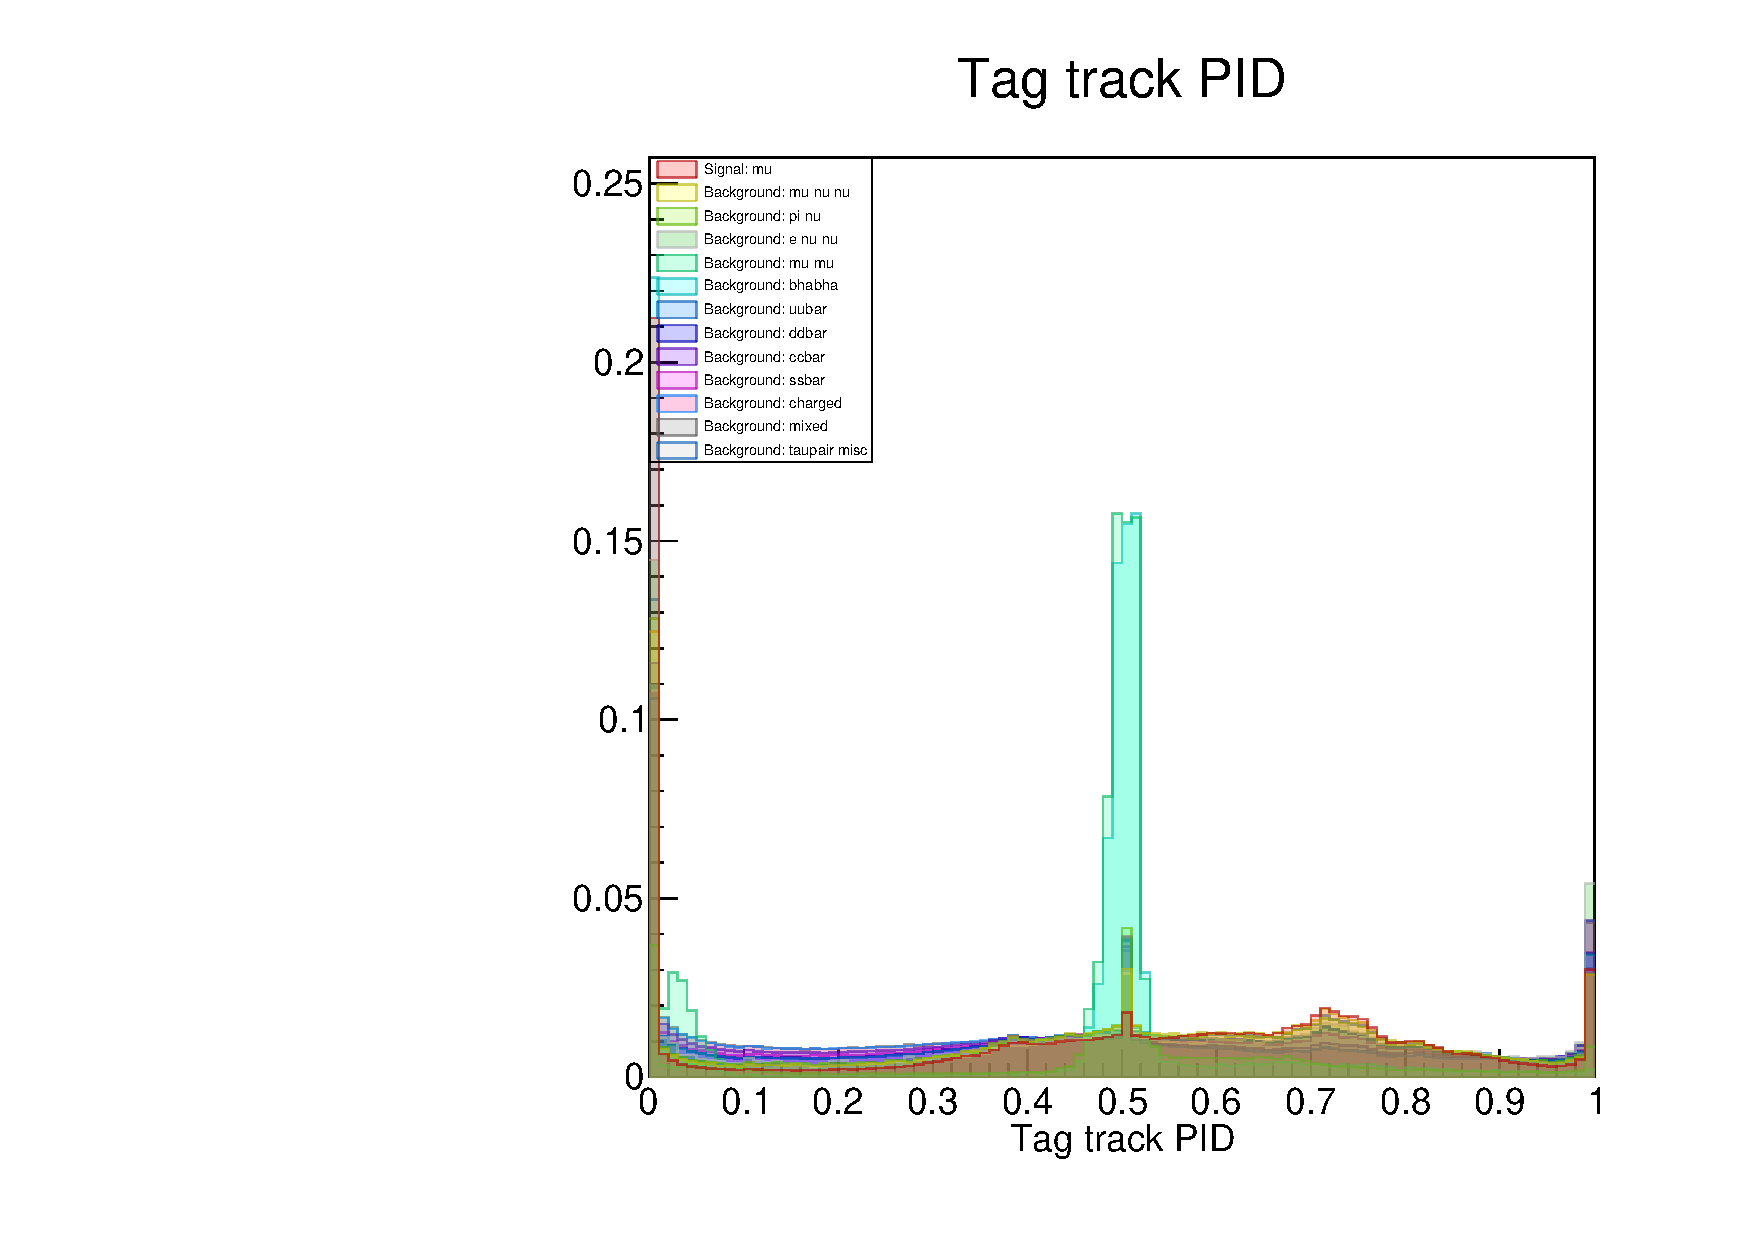
\includegraphics[width=0.5\linewidth]{images/tauMG-tagPIDmu.pdf}
\caption[]%
{{\small $\mu$-PID for tag-side track.}}
\label{fig:tagPIDmu}
\end{figure}

\subsection{Neutral particle identification}
\label{sec:neutral PID}

Long-lived neutral particles found within the Belle II detector comprise photons, neutral pions $\pi^0$ and K-long mesons $K^0_L$; only photons are important to our analysis. Photon identification relies strongly on ECL data, and is based on parameters which describe the electromagentic shower shape of ECL clusters not matched to reconstructed tracks. One of these parameters is the ratio of energy deposited in the nearest $3\times 3$ crystals to the the nearest $5 \times 5$ crystals (or E9oE25); for photons this ratio is close to 1. The main background in photon reconstruction comes from hadronic showers, which create asymmetric showers which often result in more than one ECL cluster which is not matched to a reconstructed track.


%-------------------------------------------------------------------

\section{Beam backgrounds}

Beam background is an important issue in B-factories, and especially so for the upgraded energies of SuperKEKB. Key sources of this beam background are synchrotron radiation (SR), beam-gas scattering, and Touschek radiation\cite{BelleII:tech-design-report}.

Scattered particles and photons generated by these processes collide with the beam pipe and generate showers of photons, leptons and hadrons. Additionally, other particles can be generated at the interaction point of the collision between opposite beams; these are mostly electron-positron pairs. These particles then interact with the detector, and are called beam background. This background can make searches for interesting physics events difficult, due to the large number of clusters and tracks introduced.

\subsection{Synchrotron radiation}

As charged beam particles are bent by magnets while travelling through the accelerator, they emit synchrotron radiation (SR). This radiated energy is dependent on particle momentum, and so most SR in SuperKEKB comes from the high-energy ring (HER). SR background is comprised of upstream SR directed towards the IP, and backscattering of SR from downstream. Beam backgrounds of both type have been studied and have informed the design of the interaction region to reduce its effect.

\subsection{Beam-gas scattering}	

The region inside the beam pipe is not a perfect vacuum; the designed gas pressure for SuperKEKB is $\SI{e-7}{Pa}$. Most of this gas is composed of neutral H$_2$ and CO$_2$. Beam particles can collide with the gas molecules, resulting in elastic scattering where energy is unchanged but direction is changed (Coulomb scattering), or inelastic scattering whereby a photon is emitted from the scattered particle (bremsstrahlung).

  \begin{figure}[h]
        \centering
        \begin{subfigure}[b]{0.475\textwidth}
            \centering
            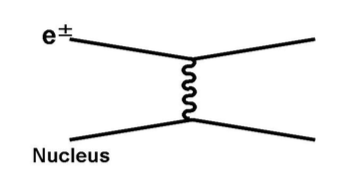
\includegraphics[width=\textwidth]{images/coulomb-scattering.png}
            \caption[]%
            {{\small Coulomb scattering.}}    
            \label{fig:coulomb scattering}
        \end{subfigure}
        \hfill
        \begin{subfigure}[b]{0.475\textwidth}  
            \centering 
            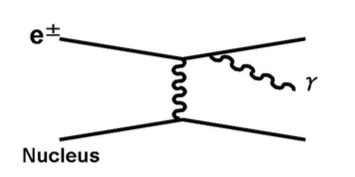
\includegraphics[width=\textwidth]{images/bremsstrahlung.png}
            \caption[]%
            {{\small Bremsstrahlung.}}    
            \label{fig:bremsstrahlung}
        \end{subfigure}
        \caption[]%
        {{\small Diagrams for beam-gas scattering in the detector.}}
    \end{figure}


\subsubsection{Coulomb scattering}

Beam electrons and positrons can elastically scatter off beam gas particles, changing direction such that the scattered particle does not reach the interaction point. Figure~\ref{fig:coulomb scattering} depicts Coulomb scattering of an electron off a beam-gas particle.

\subsubsection{Bremsstrahlung}

Beam-gas scattering can also occur as bremsstrahlung, where electrons (or positrons) recoil off gas nuclei and emit photons as shown in Figure~\ref{fig:bremsstrahlung}. The photon carries away for fraction of the scattered particle's energy.


\subsection{Touschek scattering}

Particle beams do not exist as continuous `lines' of electrons and positrons marching through the accelerator in single file. Instead, we have tightly packed beam bunches, containing $10^{10} - 10^{11}$ particles each. Bunch sizes in SuperKEKB have been greatly reduced from KEKB, which is one cause of the increased luminosity. These bunches are aligned almost perfectly parallel so that beam particles do not collide with the beam pipe during their many cycles around the accelerator.

Within these bunches the particles oscillate in a direction perpendicular to the beam trajectory, so that in addition to interacting with beam-gas, particles within a beam bunch collide with each other resulting in an transfer of energy and momentum. Trajectories of these particles may be changed by this interaction, so that they do not reach the interaction point. 

\begin{figure}
\centering
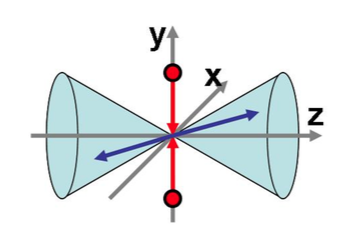
\includegraphics[width=0.5\linewidth]{images/touschek-beam-frame.png}
\caption[]%
{{\small An illustration of Touschek scattering in the bunch frame}}
\label{fig:touschek}
\end{figure}

%-------------------------------------------------------------------

\chapter{Monte Carlo production and background events}

Electron-positron collisions at Belle II will produce a wide range of different physics events. Within these, we hope to find the signal modes $\tau\to\mu\gamma$ and $\tau\to e\gamma$. However, a range of non-signal mode events are also produced; these events which are referred to as background (or sometimes physics background, distinct from beam-background) must be suppressed in order to effectively investigate signal processes. We discriminate signal from background through applying selection criteria such as energy, momentum, angular relations and event shape variables. This criteria is optimised by examining Monte Carlo (MC) simulated signal and background events. MC events are produced using physics event generators and the response of the detector is simulated.

\section{Physics backgrounds}

It is unfeasible to study MC in-depth for every possible physics background; we focus on high event rate processes and events with final states similar to our signal. In this analysis, we investigate all generically decaying tau-pair processes, mu-pair events ($e^+ e^- \to \mu^+ \mu^- (\gamma)$), Bhabha scattering ($e^+ e^- \to e^+ e^- (\gamma)$), $e^+ e^- \to q\bar{q}$ events (where $q = u, d, c, s$) usually referred to as continuum background, and generic B$\bar{\text{B}}$ processes ($e^+ e^- \to B^+ B^-$ or $e^+ e^- \to B^0 \bar{B}^0$). Of the tau-pair processes, we isolate the modes $\tau \to \mu \nu \nu$, $\tau \to e \nu \nu$, and $\tau \to \pi \nu$ (for charged pions $\pi^{\pm}$) for investigation, as these have the largest branching fractions of generic $\tau$ decays. Feynman diagrams of the backgrounds are shown in Figure~\ref{fig:background feynman diagrams START} -~\ref{fig:background feynman diagrams END}. Note that $e^+ e^- \to B\bar{B}$ proceeds though production of the meson $\Upsilon(4S)$.


  \begin{figure}
        \centering
        \begin{subfigure}[b]{0.315\textwidth}
            \centering
            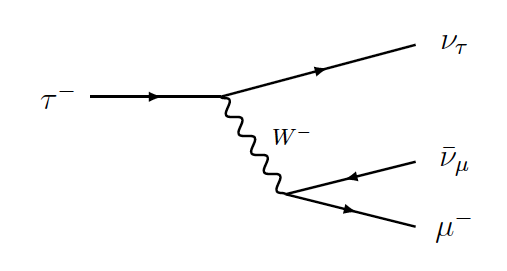
\includegraphics[width=\textwidth]{images/taumununu.png}
            \caption[Network2]%
            {{\small $\tau^-\to \mu ^-\nu_{\mu} \nu_{\tau}$}}    
            \label{fig:background feynman diagrams START}
        \end{subfigure}
        \hfill
        \begin{subfigure}[b]{0.315\textwidth}  
            \centering 
            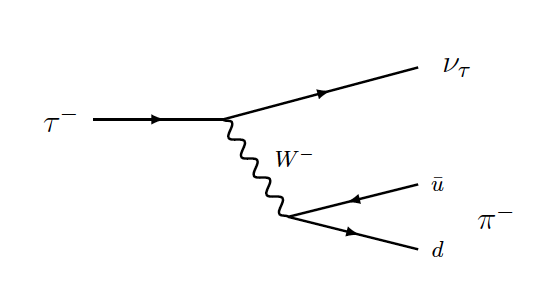
\includegraphics[width=\textwidth]{images/taupinu.png}
            \caption[]%
            {{\small $\tau^-\to \pi^- \nu_{\mu}$}}    
        \end{subfigure}
                \hfill
        \begin{subfigure}[b]{0.315\textwidth}  
            \centering 
            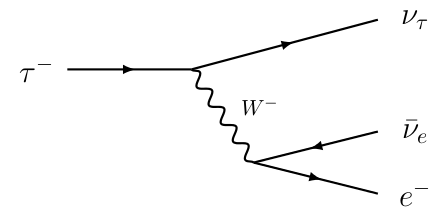
\includegraphics[width=\textwidth]{images/enunu.png}
            \caption[]%	
            {{\small $\tau^-\to e^- \nu_{e}\nu_{\tau}$}}    
        \end{subfigure}
        \vskip\baselineskip\vspace{0.4cm}
                \begin{subfigure}[b]{0.315\textwidth}
            \centering
            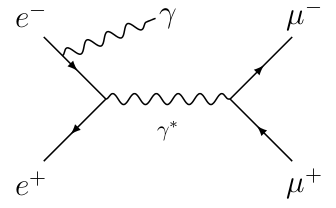
\includegraphics[width=0.8\textwidth]{images/mupair.png}
            \caption[]%
            {{\small $e^+ e^- \to \mu^+ \mu^- \gamma$}}   
            \label{fig:feynman radiative mu-pair} 
        \end{subfigure}
        \begin{subfigure}[b]{0.315\textwidth}  
            \centering 
            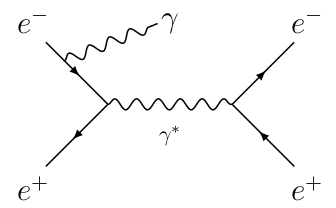
\includegraphics[width=0.8\textwidth]{images/bhabha.png}
            \caption[]%
            {{\small $e^+ e^- \to e^+ e^- \gamma$}}    
            \label{fig:background feynman diagrams END}
        \end{subfigure}
        \caption[]%
        {{\small Feynman diagrams for the dominant leptonic physics backgrounds for $\tmg$.
        The radiative photon mu-pair and Bhabha processes in~\ref{fig:feynman radiative mu-pair} and~\ref{fig:background feynman diagrams END} can originate from any of the four charged particles. We analyse both radiative and non-radiative (without a final state photon) processes in this analysis.}} 
        \label{fig:background feynman diagrams}
    \end{figure}


Fiducial cross-sections for these backgrounds are given in Table~\ref{tab:background cross-sections}. These values are for collisions at center-of-mass beam energies of $\SI{10.573}{GeV}$ and with Belle II detector geometry.


\begin{table}[h]
\centering
\begin{tabular}{lll}
\hline 
\textbf{Background process} & \textbf{Cross-section [nb]} & \textbf{Generator} \\
\hline
$\tau \to \mu\nu\nu$ & \num{0.160} & \texttt{KKMC}, \texttt{TAUOLA} \\
$\tau \to \pi\nu$ & \num{0.100} & \texttt{KKMC}, \texttt{TAUOLA} \\
$\tau \to e\nu\nu$ & \num{0.164} & \texttt{KKMC}, \texttt{TAUOLA}  \\
$\tau \to \text{generic}$ & \num{0.919} & \texttt{KKMC}, \texttt{TAUOLA} \\
$e^+e^- \to \mu^+\mu^-(\gamma)$ & \num{1.148} & \texttt{KKMC} \\
$e^+e^- \to e^+e^-(\gamma)$ & \num{300} & \texttt{BABAYAGA.NLO}   \\ \hline
$e^+e^- \to u\bar{u}$ & \num{1.61} & \texttt{KKMC} \\
$e^+e^- \to d\bar{d}$ & \num{0.40} & \texttt{KKMC} \\
$e^+e^- \to s\bar{s}$ & \num{0.38} & \texttt{KKMC} \\
$e^+e^- \to c\bar{c}$ & \num{1.30} & \texttt{KKMC} \\
$e^+e^- \to B^+B^-$ & \num{0.525} & \texttt{EvtGen 1.3}, \texttt{PYTHIA 8.2} \\
$e^+e^- \to B^0\bar{B}^0$ & \num{0.525} & \texttt{EvtGen 1.3}, \texttt{PYTHIA 8.2} \\ \hline
\end{tabular}
\caption[]%
{{\small Fiducial cross-sections for backgrounds at Belle II.}}
\label{tab:background cross-sections}
\end{table}


\section{Event generation}

All MC was generated in the Belle II Analysis Framework (basf2) with geometry and energies from SuperKEKB using physics event generators given in Table~\ref{tab:background cross-sections}. All generators use the same beam parameters such as vertex positions and beam energies, as well as geometry information including highly accurate location, thickness and material values. Magnetic field strength through the detector is also known and included in event generation. The detector components are simulated by the generator, so that timing information and energy deposition is recorded for these components as MC particles interact with them. Following the simulation of a physics event, information from the sub-detectors is used to reconstruct tracks (correponding to charged particles) and clusters (referring to cells of the ECL with which a particle has interacted with, corresponding to photons).

\subsection{Signal generation}

Signal MC was produced using the \texttt{KKMC} generator, the default generator for tau-pair and mu-pair final state processes $e^+ e^-\to\mu^+ \mu^-(\gamma)$ and $e^+ e^- \to \tau^+ \tau^- (\gamma)$~\cite{BelleII:simulation}. Decays proceeded as $e^+ e^- \to \tau^+ \tau^-$, with one tau decaying to the signal mode $\tau \to \ell \gamma$ (the signal-side), and the other (the tag-side) decaying to all experimentally measured SM decay modes of the $\tau$ (called generic decay), scaled by their branching ratio. $\tau^+ \to \ell^+ \gamma$ and $\tau^- \to \ell^- \gamma$ modes were both generated to account for differences due to charge. A total of \num{3100000} events were generated for the muon mode, and \num{2550000} for the electron mode.

\subsection{Background generation}

Samples for a range of background events were produced by the Belle II collaboration; the generators used for each background process are given in Table~\ref{tab:background cross-sections}. Initial state radiation (ISR) and final state radiation (FSR) of multiple photons is generated by \texttt{KKMC} and \texttt{BABAYAGA.NLO} generators. Beam backgrounds are not generated using standard event generators are given in Table~\ref{tab:background cross-sections} and are instead generated using dedicated software then later mixed with physics background MC.

\section{Event scaling}

Belle II is projected to collect a time-integrated luminosity of $\SI{50}{ab^{-1}}$ over the length of the experiment. Instead of running over the equivalent amount of background events expected in such a sample size we can run over a smaller number of events then scale results. This is done for computing reasons, as the number of background events recorded for these luminosities quickly becomes prohibitively large.

We choose to scale up to a luminosity of $\SI{1}{ab^{-1}}$; this is the total time-integrated luminosity of the complete Belle dataset, and so is useful as a point of comparison to previous searches. The scale factor for each event type is calculated by

\begin{equation}
n_{\SI{1}{ab^{-1}}} = n_{\text{generated}} \times \text{scale factor},
\end{equation}

where $n_{\SI{1}{ab^{-1}}}$ = $\mathcal{L} \sigma$, and $n_{\text{generated}}$ is the number of events generated. Scaled event numbers are presented in Table~\ref{tab:scaled event numbers} below.

\begin{table}[h]
\centering
\begin{tabular}{lrrr}
\textbf{Event type} & $\mathbf{n_{\text{generated}}}$ & \textbf{scale factor} & $\mathbf{n_{\SI{1}{ab^{-1}}}}$ \\ \hline
\rowcolor[HTML]{EFEFEF} 
$\tau \to \mu\gamma$ & \num{3200000} & \num{2.58e-05} & \num{83} \\
\rowcolor[HTML]{EFEFEF}
$\tau \to e\gamma$ & \num{2550000} & \num{8.65E-05} & \num{221} \\       
$\tau \to \mu\nu\nu$ & \num{127998320} & \num{1.250} & \num{159997900} \\
$\tau \to \pi\nu$ & \num{267245200} & \num{1.250} & \num{334056500}  \\
$\tau \to e\nu\nu$ & \num{131086160} & \num{1.250} & \num{163857700}  \\
$\tau \to \text{generic}$ & \num{208870320} & \num{1.250} & \num{261087900} \\
$e^+e^- \to \mu^+\mu^-(\gamma)$ & \num{148600000} & \num{7.725} & \num{1148000000}  \\
$e^+e^- \to e^+e^-(\gamma)$ & \num{15630000} & \num{19193.858} & \num{300000000000}  \\
$e^+e^- \to u\bar{u}$ & \num{1268991935} & \num{1.269} & \num{1610000000} \\
$e^+e^- \to d\bar{d}$ & \num{317048262} & \num{1.262} & \num{400000000} \\
$e^+e^- \to c\bar{c}$ & \num{1039855756} & \num{1.250}  & \num{1300000000} \\
$e^+e^- \to s\bar{s}$ & \num{289900586} & \num{1.310}  & \num{380000000}  \\
$e^+e^- \to B^+B^-$ & \num{451320000} & \num{1.219}  & \num{550000000}  \\
$e^+e^- \to B^0\bar{B}^0$ & \num{427680000} & \num{1.286}  & \num{550000000} 
\end{tabular}
\caption{Scaled event numbers}
\label{tab:scaled event numbers}
\end{table}

Unless explicitly stated, scaled event numbers will be used throughout this analysis as to provide accurate points of comparison between events.


\section{Version differences}

The software framework on which event generation was performed is undergoing continuous development; a majority of signal and background MC was produced on the same release version to ensure accuracy between MC types. This version was made available on July 13th 2016, and was one of the most up-to-date releases at the time of analysis. However, the backgrounds $\mu^+\mu^-(\gamma)$ and $e^+ e^-(\gamma)$ (mu-pair and bhabha, respectively) did not have any events generated using this release, and instead used an older release dated August 4th 2015.

A full investigation into the differences in generated MC between releases has not been performed in this analysis, as it is assumed they are negligible in most relevant cases. Changes relate mostly to the mixing of beam backgrounds; however one major change is in the reporting of timing data from the ECL. From the release dated July 13th 2016 onwards, these associated times will be reported in nanoseconds, rather than uncalibrated clock ticks\cite{BelleII:cluster-timing}. In comparing samples of background MC generated in both the older and newer releases, Figure~\ref{fig:cluster timing old} and~\ref{fig:cluster timing new} below, as well as private correspondance with the developer responsible for these changes, it was found that conversion to the newer scale could be achieved by adding 80 units to the cluster timing values.


   \begin{figure}[h]
        \centering
        \begin{subfigure}[b]{0.475\textwidth}
            \centering
            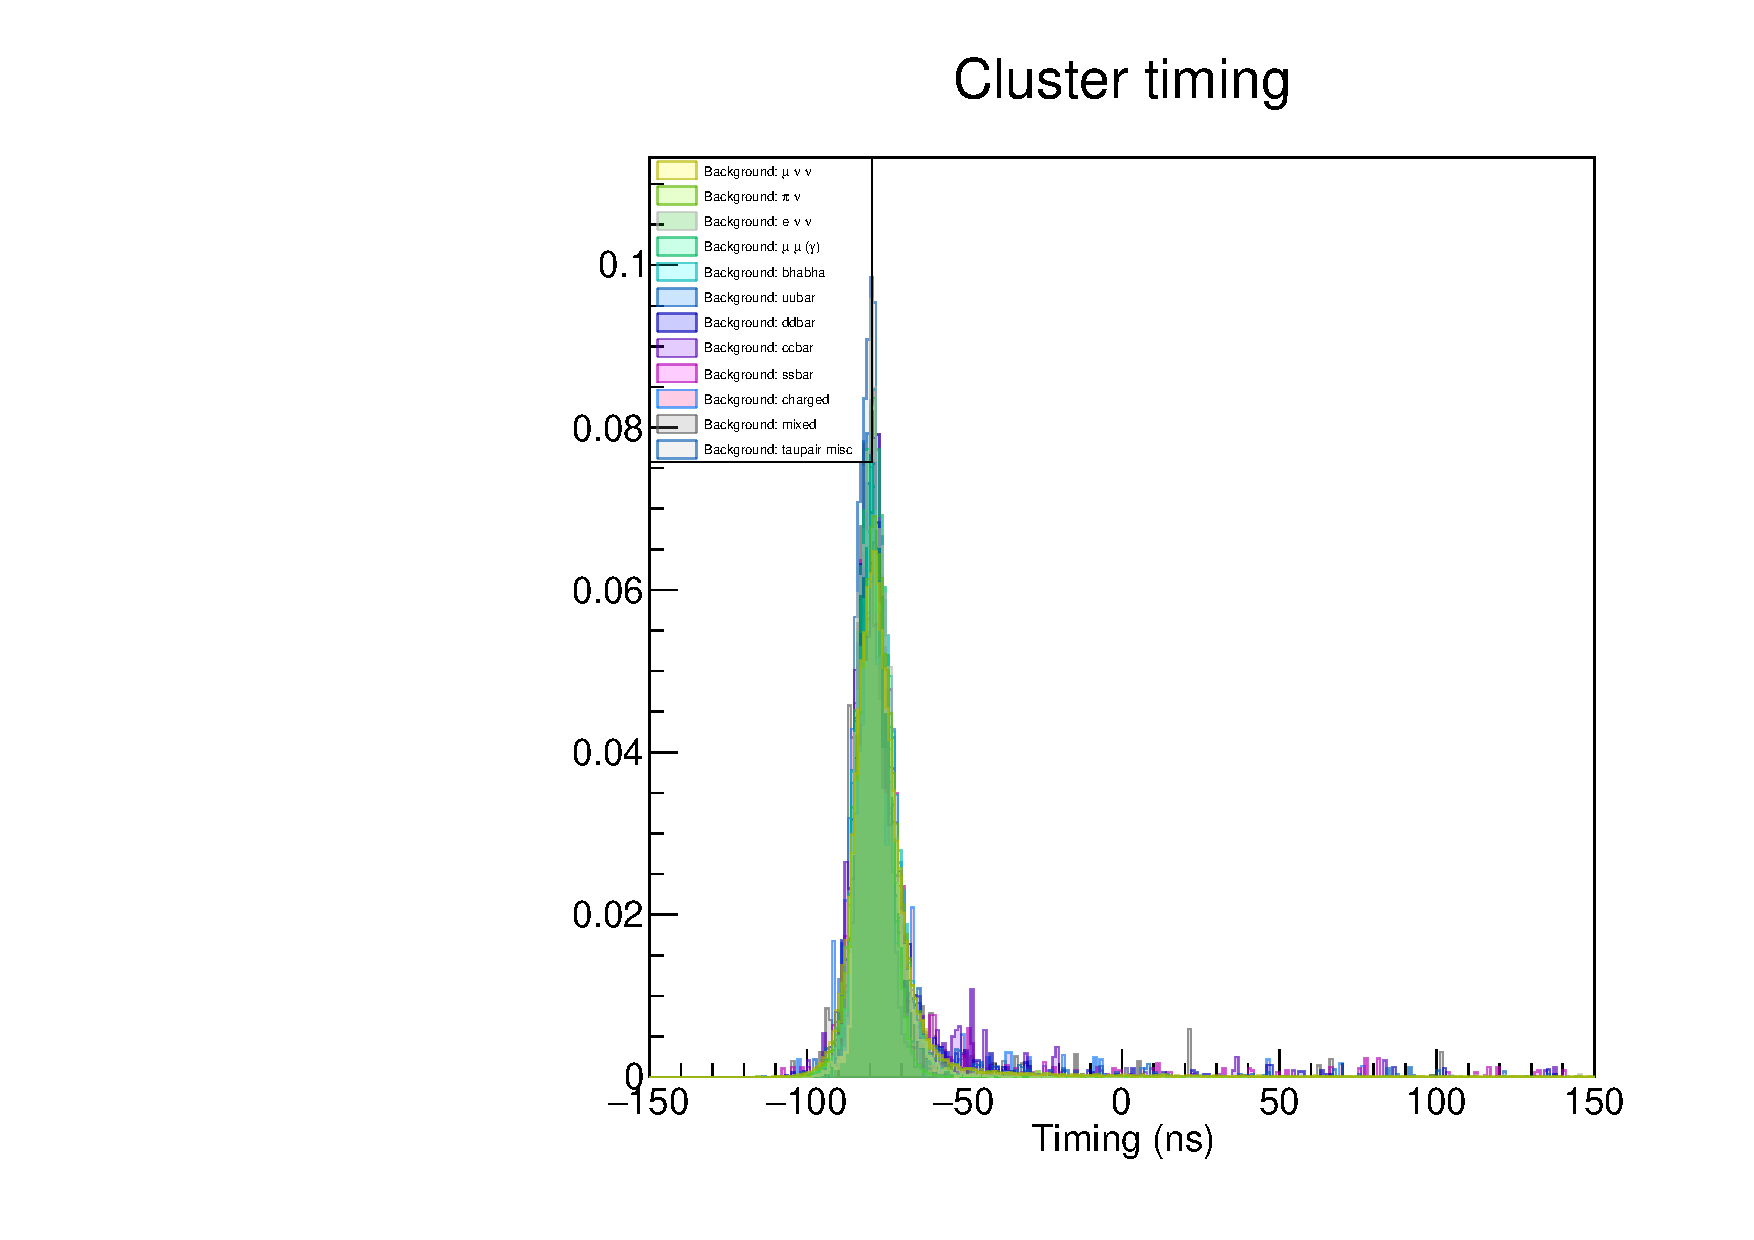
\includegraphics[width=\textwidth]{images/cluster-timing-old.pdf}
            \caption[]%
            {{\small}}    
            \label{fig:cluster timing old}
        \end{subfigure}
        \begin{subfigure}[b]{0.475\textwidth}  
            \centering 
            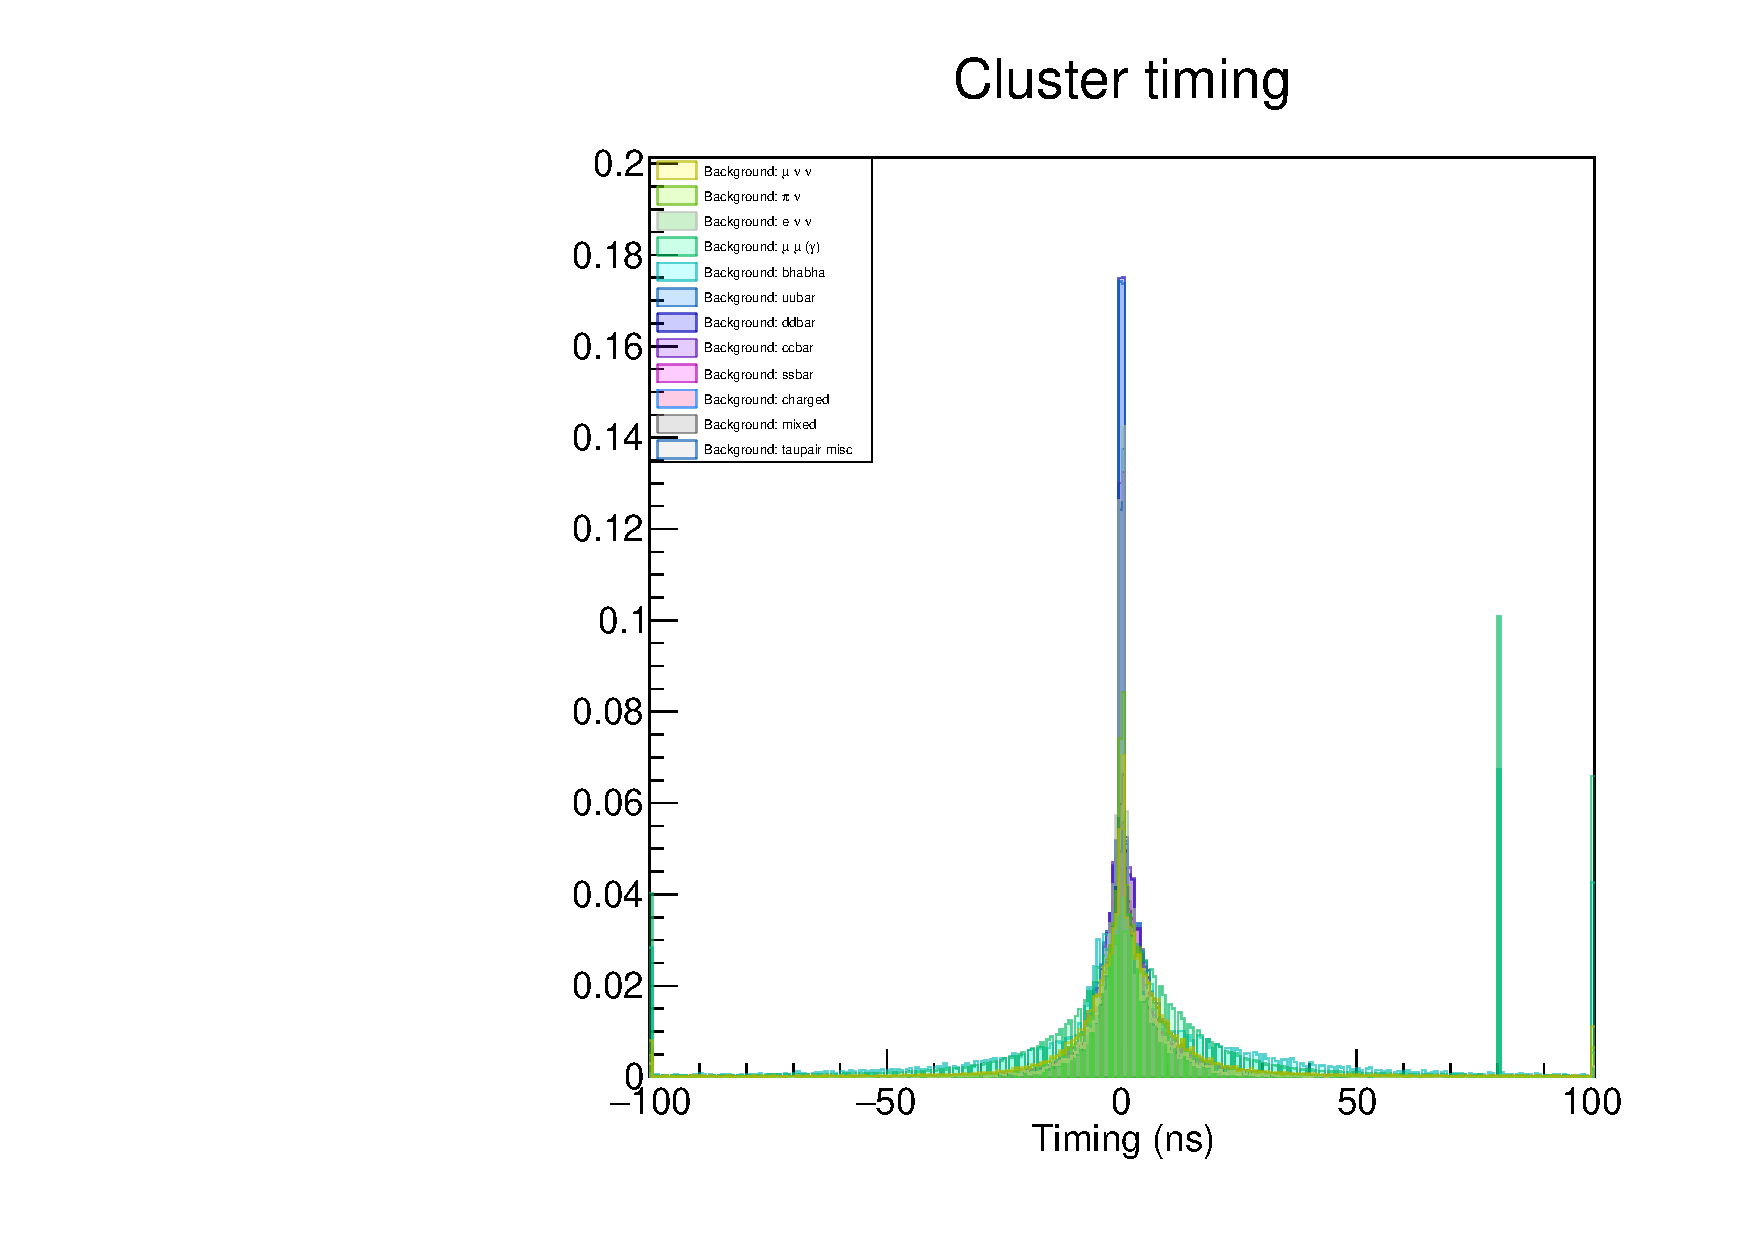
\includegraphics[width=\textwidth]{images/cluster-timing-new.pdf}
            \caption[]%
            {{\small}}    
            \label{fig:cluster timing new}
        \end{subfigure}
        \caption{Comparisons of cluster timing with background MC (a) prior to ECL timing change and (b) after ECL timing change. Note the shift in peak by 80 units between versions.}
        \label{fig:cluster timing comparison}
    \end{figure}



\section{Implementation of beam backgrounds}

Signal and background MC was generated with simulated beam background. The most important sources have been generated by a dedicated accelerator group software within the Belle II collaboration. This software simulates particles travelling the detector and records the position and momentum of particles which leave the nominal beam trajectory and collide with the beam pipe of beam collimator. Detector response simulation is then processed for these particles to produce background samples of a given type. Separate backgrounds were made for electron (HER) and positron (LER) beams, due to differences in energies and currents. Implemented background types are listed in Table~\ref{tab:beam background types}.


\begin{table}[h]
\centering
\begin{tabular}{lcr}
\hline
\multicolumn{1}{c}{type}      & source & \multicolumn{1}{c}{rate [MHz]} \\ \hline
radiative Bhabha              & HER    & \num{1320}                     \\
radiative Bhabha              & LER    & \num{1294}                     \\
radiative Bhabha (wide angle) & HER    & \num{40}                       \\
radiative Bhabha (wide angle) & LER    & \num{85}                       \\
Touschek scattering           & HER    & \num{31}                       \\
Touschek scattering           & LER    & \num{83}                       \\
beam-gas interactions         & HER    & \num{1}                        \\
beam-gas interactions         & LER    & \num{156}                      \\ \hline
\end{tabular}
\caption[]%
{{\small Beam background types simulated at Belle II. Rate is calculated as number of events per second at Belle II standard operating luminosity\cite{BelleII:simulation}.}}
\label{tab:beam background types}
\end{table}


For comparison, some samples of MC were generated without beam background. Comparisons between some measureables are shown in Figures~\ref{fig:tracks w/o beam background} and~\ref{fig:tracks w/ beam background}, ~\ref{fig:uubar tagtrackP beambackground} and ~\ref{fig:uubar neutralEclEnergy beambackground} below.

   \begin{figure}[h]
        \centering
        \begin{subfigure}[b]{0.475\textwidth}
            \centering
            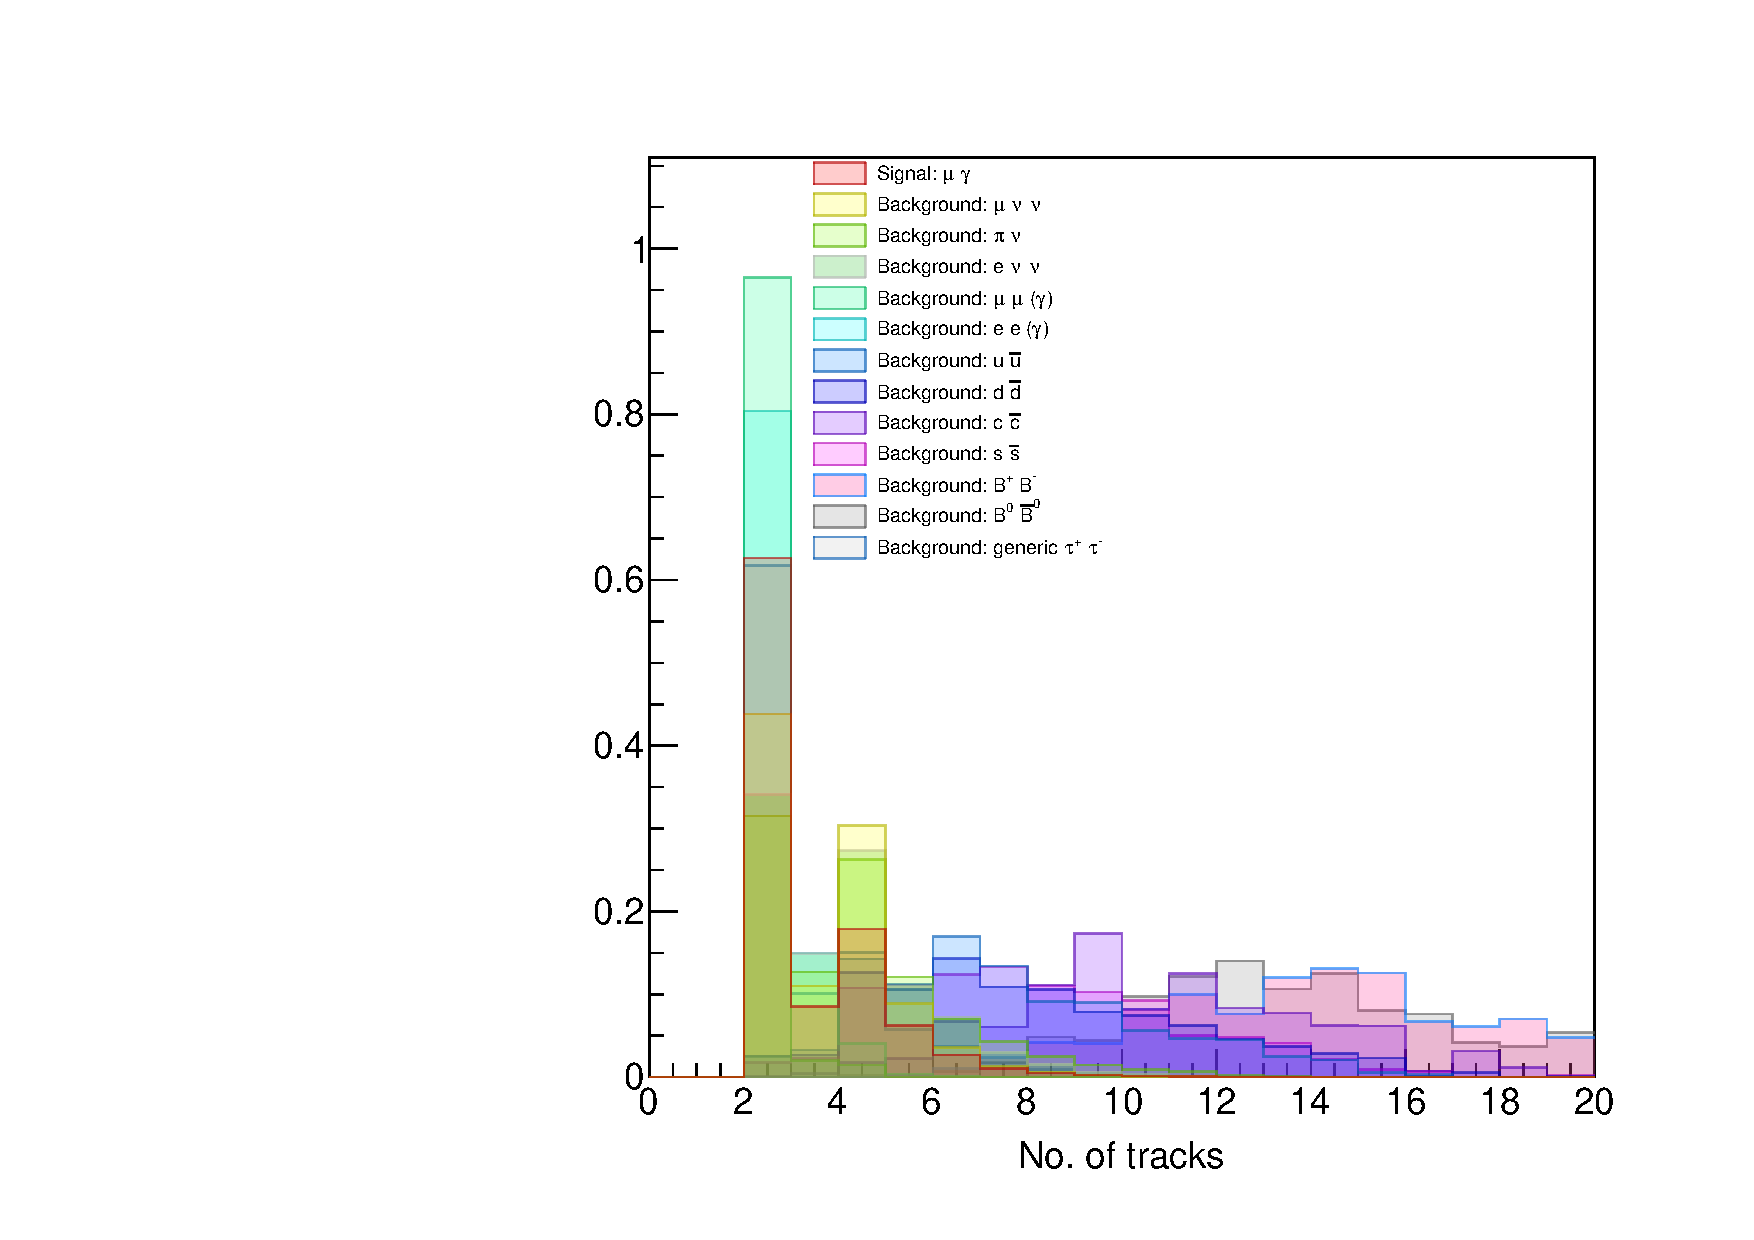
\includegraphics[width=\textwidth]{images/tauMG-tracks-BGx0.pdf}
            \caption[]%
            {{\small Number of tracks, without beam background mixing.}}
            \label{fig:tracks w/o beam background}   
        \end{subfigure}
        \hfill
        \begin{subfigure}[b]{0.475\textwidth}  
            \centering 
            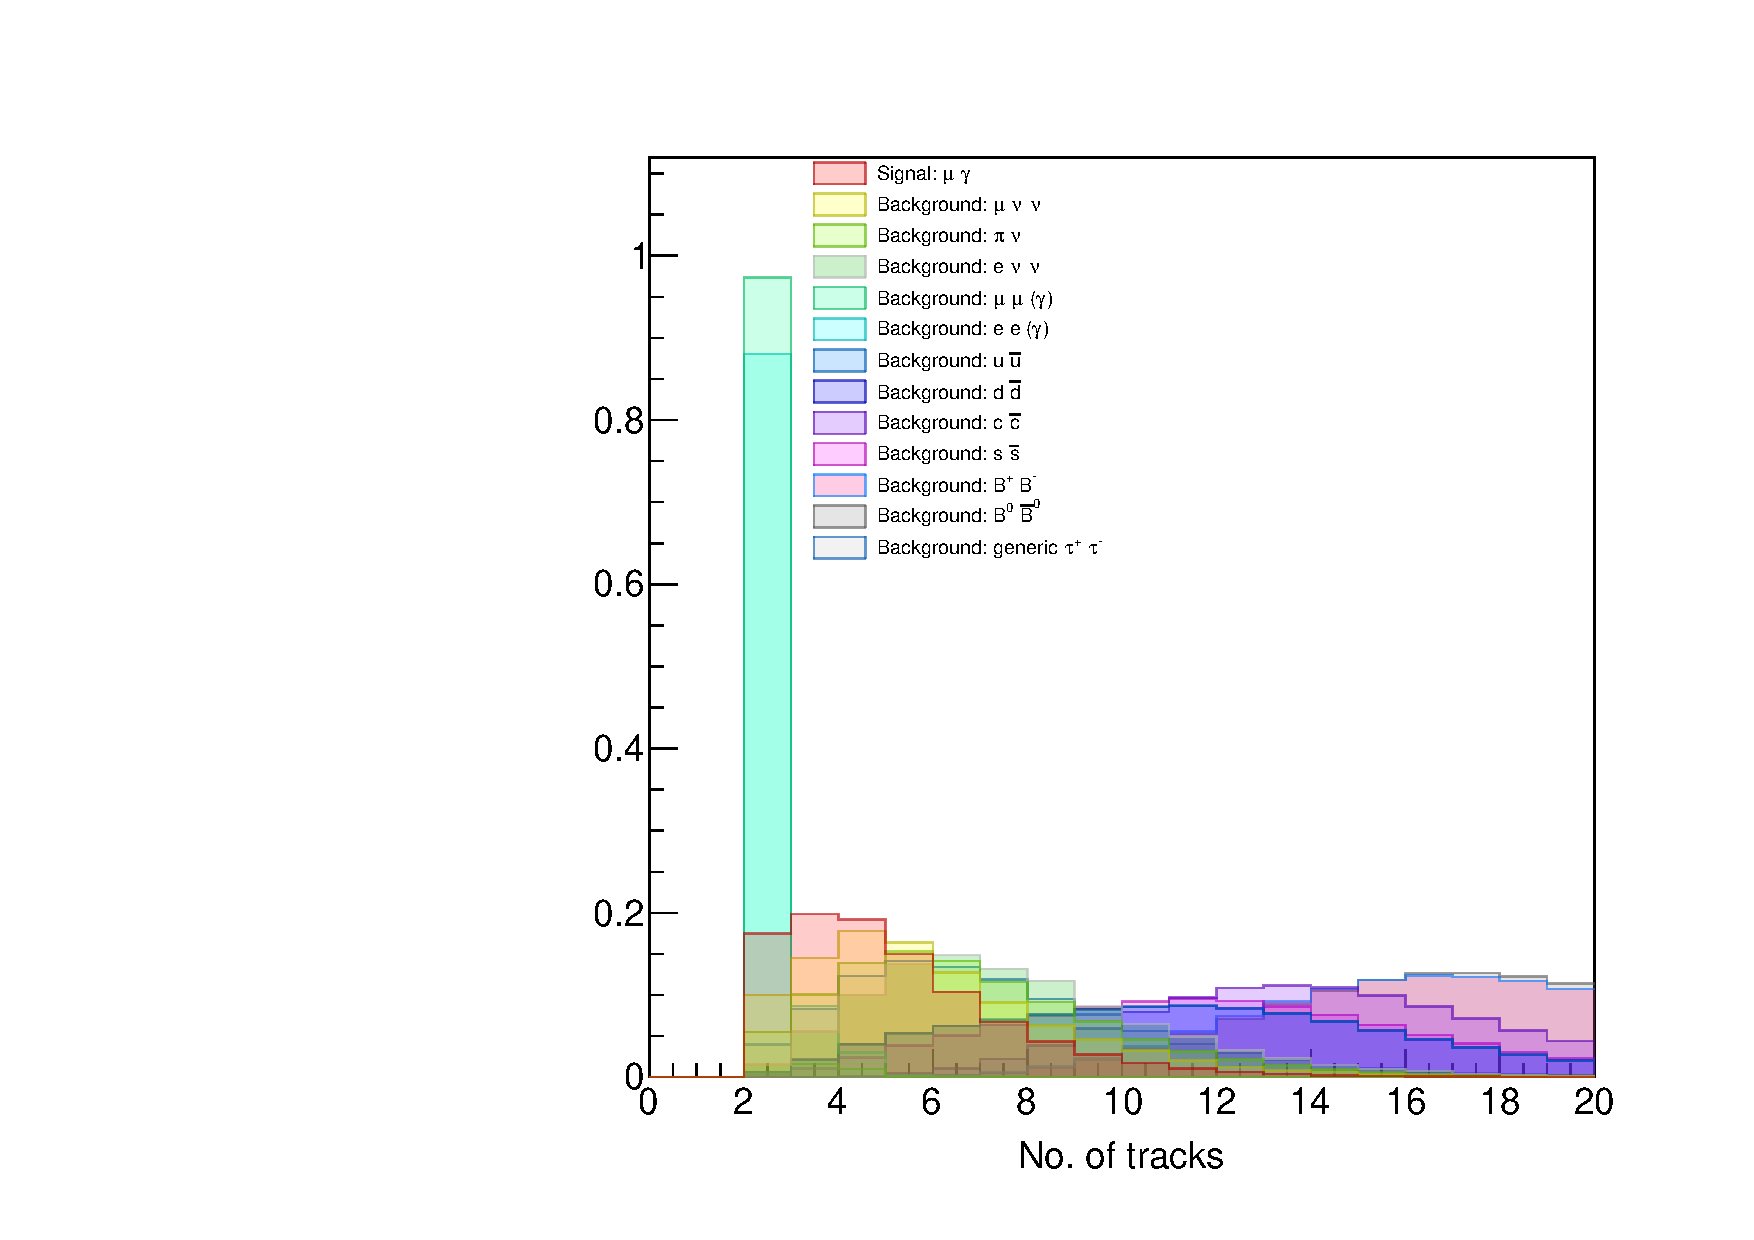
\includegraphics[width=\textwidth]{images/tauMG-tracks.pdf}
            \caption[]%
            {{\small Number of tracks, with beam background mixing.}}    
            \label{fig:tracks w/ beam background}
        \end{subfigure}
        \caption[]%
        {{\small Comparison of number of tracks for signal and background distributions with and without beam background mixing.}}
    \end{figure}
    
    
\begin{figure}
\centering
\begin{minipage}{.475\textwidth}
  \centering
  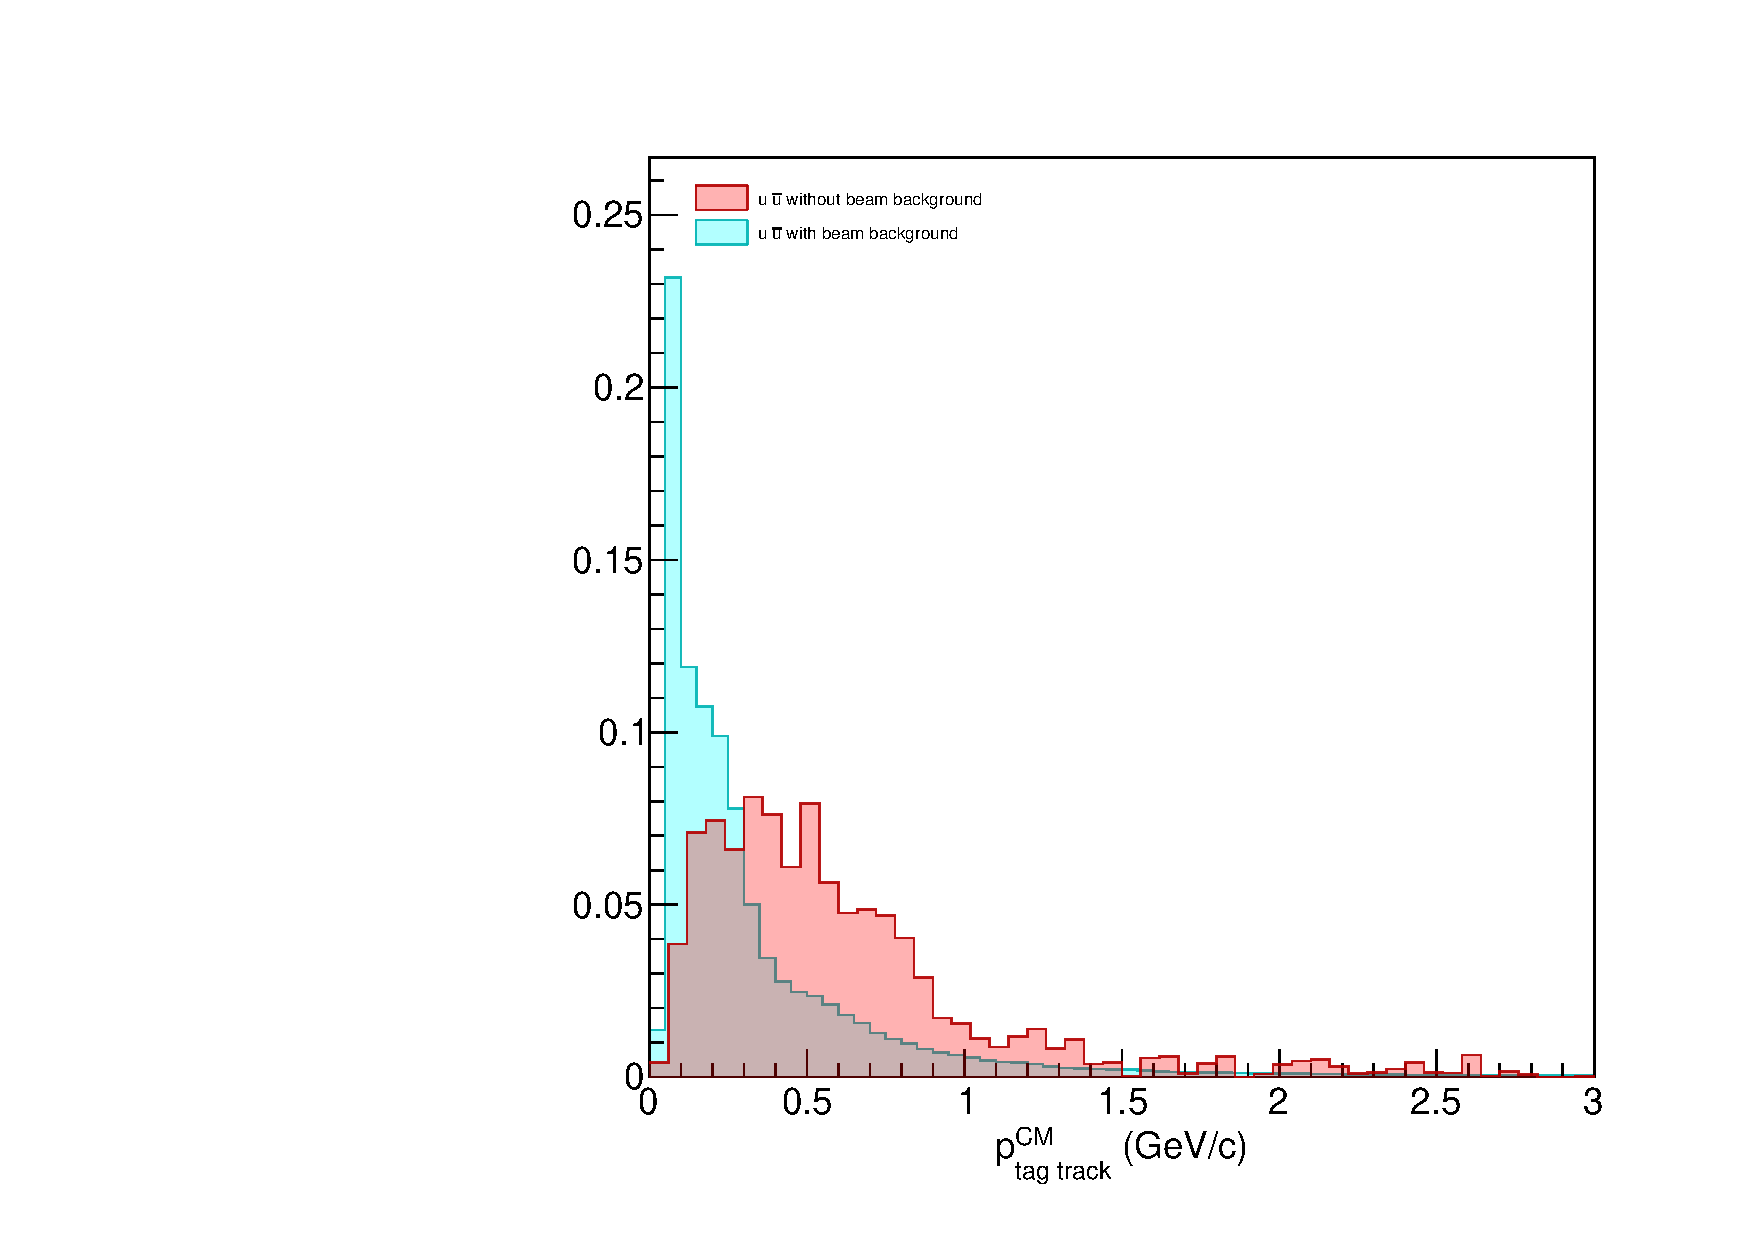
\includegraphics[width=\linewidth]{images/uubar-tagtrackP-beambackground.pdf}
  \caption[]%
  {{\small Comparison of tag-track momentum for $u\bar{u}$ events, with and without beam background mixing.}}    
  \label{fig:uubar tagtrackP beambackground}
\end{minipage}%
        \hfill
\begin{minipage}{.475\textwidth}
  \centering
  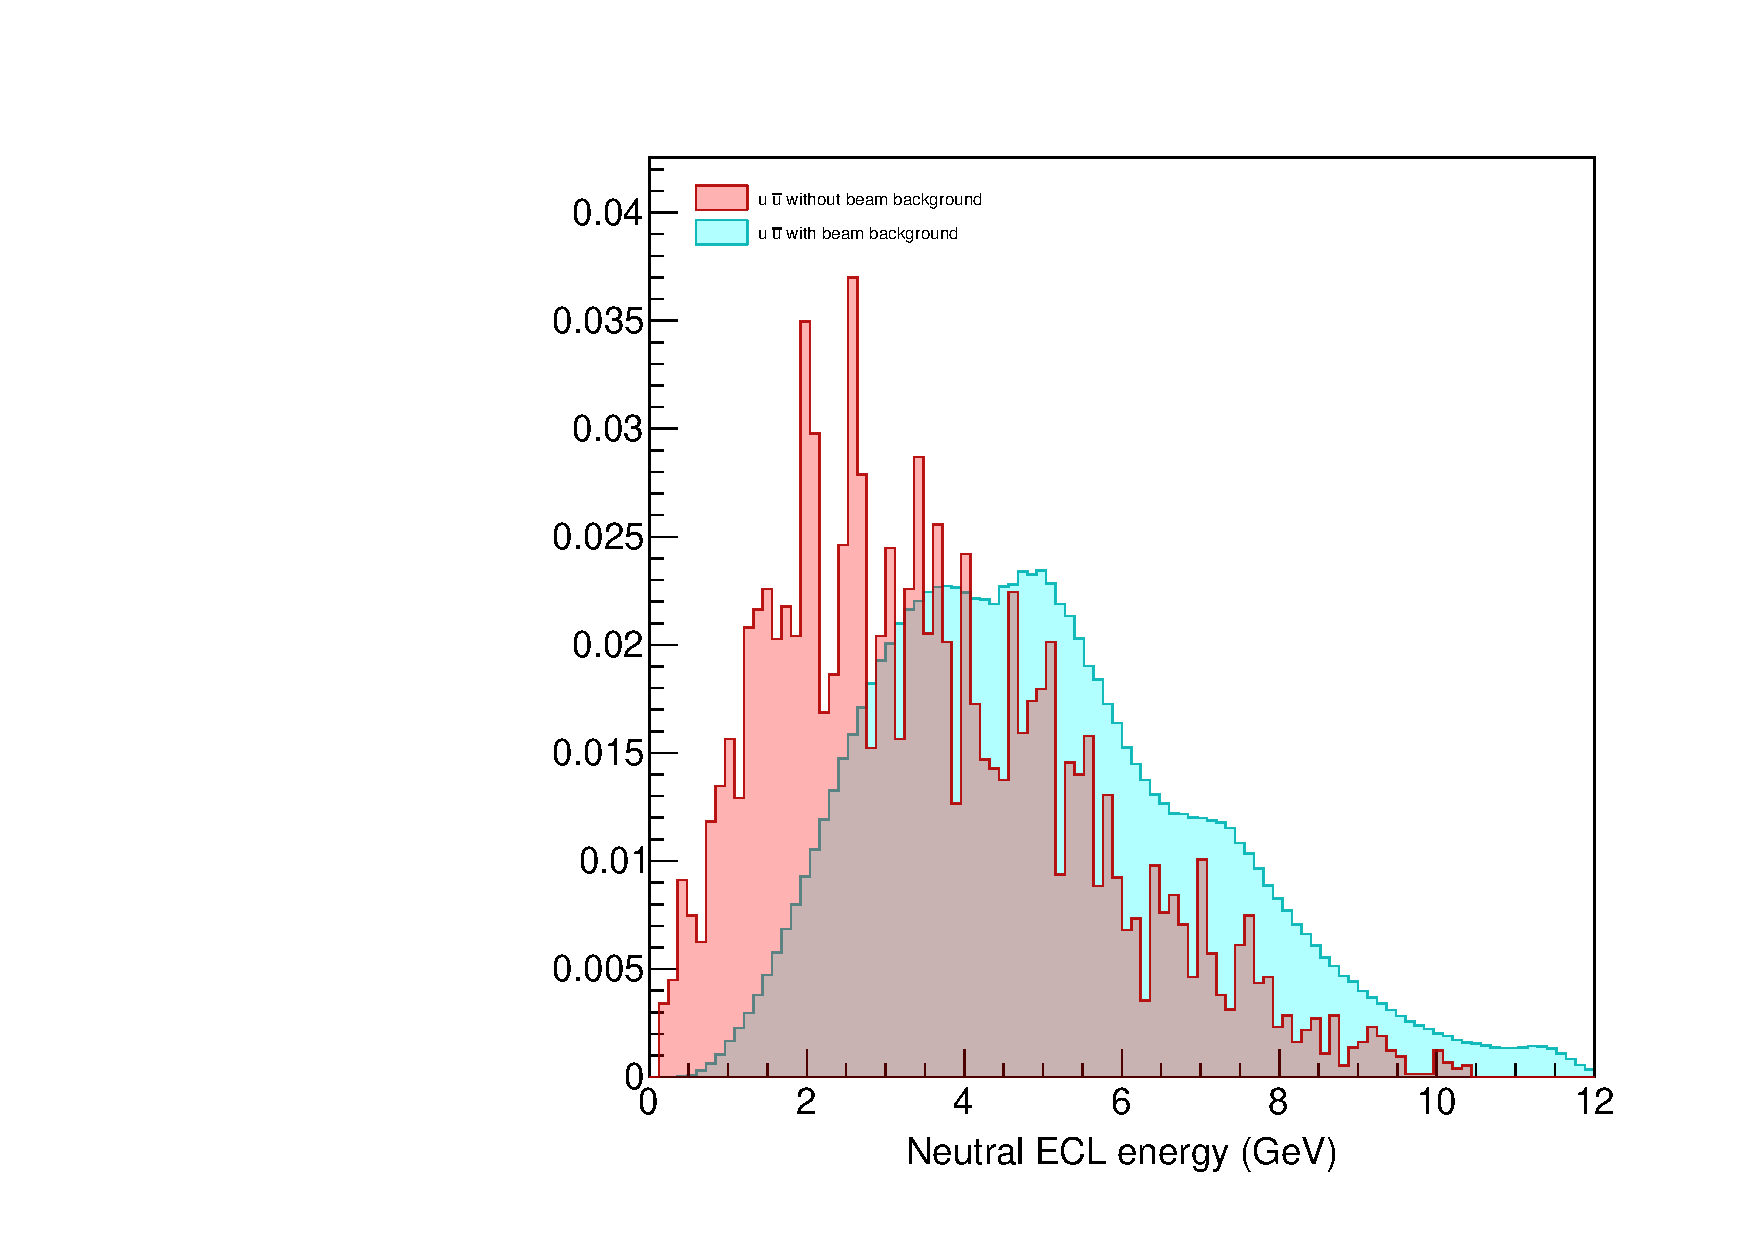
\includegraphics[width=\linewidth]{images/uubar-neutralEclEnergy-beambackground.pdf}
  \caption[]%
  {{\small Comparison of total energy deposited in all ECL clusters by neutral particles for $u\bar{u}$ events, with and without beam background mixing.}}  
  \label{fig:uubar neutralEclEnergy beambackground}
\end{minipage}
\end{figure}
    
    
There are many differences between MC with and without beam background; only a few key points will be discussed here. Most obvious is the number of tracks recorded. Taking, for instance, our signal mode, we would expect for most events 2 or 4 tracks - one signal-side track corresponding to $\mu/e$, and one or three tracks on the tag-side (one- or three-pronged) coming from standard model $\tau$ decays, which are dominantly one- or three-pronged. Beam background particles in the detector produce a number of new tracks (as well as clusters) which are tracked by sub-detector components, then later reconstructed.

Kinematic variables such as energy and momentum are also obviously affected by beam background. We observe an increase in low energy and low momentum tracks - the shift in momentum peak in Figure~\ref{fig:uubar tagtrackP beambackground} is due to particles from beam background being reconstructed as tag-side tracks. In Figure~\ref{fig:uubar neutralEclEnergy beambackground} the energy variable distribution has been shifted by $\sim\SI{2}{GeV}$ in the beam background case, while the shape of the distribution is mostly unchanged. Production of photons through beam background processes cause an additional $\sim\SI{2}{GeV}$ to be deposited in the ECL. Note that the the non-beam background MC has limited statistics, resulting in ``jagged'' distributions.



\pagebreak
%------------------------------------------------------------------

\chapter{Reconstruction}

Reconstruction of events can be separated into three sections --- tracking, calorimeter reconstruction, and particle identification (the latter of which is discussed in Section~\ref{sec:PID}) \cite{BelleII:reconstruction}.

Tracking of charged particle is achieved using the innermost detectors, the VXD and the CDC. Pattern recognition algorithms are to collect all detector hits belonging to a single track, then a track candidate is created. Impact parameters can be determined through the VXD, and hence vertex positions of decaying particles can be calculated. A helical fit is applied to the track candidate, using track impact parameters combined with highly accurate measurements of charged track momenta from the CDC. The track is extrapolated from the CDC to the point-of-closest approach (POCA).

Energies and positions of depositions from neutral and charged particles are reconstructed using the calorimeter information. This reconstruction is primarily for photons, though can be used for neutral hadrons such as $\pi^0$. Clustering of cells is performed algorithmically, beginning with a cluster of at least $\SI{10}{MeV}$ energy deposited and is a local energy maximum among all nearest neighbour cells (cell which touch a side of a corner of the crystal). The cluster is then populated with all nearest and nest-to-nearest neighbours of the seed crystal. The central position $\vec{x}$ of the cluster is calculated using the linear weights of the crystals,
\begin{equation}
\vec{x}=\frac{\sum_i E_i \vec{x}_i}{\sum_i E_i},
\end{equation}
where $E_i$ and $\vec{x}_i$ are the energy deposits and central positions of the $i$-th crystal in the cluster. Cluster energy is reconstructed as the linear sum of all included crystals. Clusters are matched to extrapolated tracks in the case that a crystal in the cluster is hit by the track. All other clusters are then associated with a photon or a neutral hadron as discussed in Section~\ref{sec:neutral PID}.


\section{Reconstruction criteria}

To reconstruct events in basf2, we first fill lists of charged particles and photons reconstructed as described above. Particles must pass loose selection of particle identification to populate the lists --- muon candidates require $\mu$-PID values greater than 0.1, and similar for electrons and pions. Photon candidates are also required to have probability likelihood greater than \num{0.5}.

We define the signal track to be reconstructed track associated with the final state electron or muon from $\tau\to\ell\gamma$; similarly the signal photon describes the cluster associated with the final state photon. The signal-side particles do not necessarily refer to the physical charged particle or photon coming from the signal modes under analysis; misidentified particles (such as a pion being identified as a muon during reconstruction) or particles from different decay processes (such as a muon from the tau process $\tau\to\mu\nu\nu$).

We reconstruct the signal side $\tau$ as $\tau \to \mu (e) \gamma$ for the muon (electron) mode. The tag side $\tau$ is reconstructed by from at least one muon, electron or charged pion. In addition to PID requirements, we also apply loose selection on $\Delta E$ and $M_{\text{inv}}$. These are our signal region variables on which final event selection will be performed; we define our signal region variables as
\begin{align}
\Delta E &= E^{\text{CM}}_{\text{signal }\tau} - E_{\text{beam}}/2,\\
M_{\text{inv}} &= \text{invariant mass of reconstructed signal-side $\tau$},
\end{align}
where $E^{\text{CM}}_{\text{signal }\tau}$ is the center-of-mass energy of the reconstructed signal-side tau, and $E_{\text{beam}}$ is the total center-of-mass energy of the electron-positron beam system. Nominally we expect signal events to have $\Delta E\sim 0$ and $M_{\text{inv}}\sim m_{\tau}$. As to not bias final event selection, we place only loose requirements on the signal region variables, requiring $\SI{-0.4}{GeV} < \Delta E < \SI{0.2}{GeV}$ and $\SI{1.6}{GeV} < M_{\text{inv}} < \SI{1.9}{GeV}$ for the signal-side $\tau$. 

\section{Reconstruction efficiencies}

The number of events over which reconstruction was performed, and the reconstruction efficiency $\epsilon_{\text{recon}}$, is shown in Table~\ref{tab:muon mode reconstruction values}. Reconstruction efficiencies for $\tau\to\mu\gamma$ and $\tau\to e\gamma$ are shown to be greater than $\SI{100}{\percent}$. This is due to some signal events having multiple candidates --- there are multiple combinations of tracks and clusters in the event which can reconstruct the signal- and tag-side $\tau$'s. No explicit requirements are made as to remove this double-counting, such as only reconstructing the best candidate for an event. Instead we rely on preselection and selection criteria to remove these extra candidates; further study could be undertaken to investigate the effect of this double-counting on the analysis, or to find the best method of selection a signal candidate.

\begin{table}[h]
\centering
\begin{tabular}{lrrr}
\textbf{Event type}         & \textbf{events in} & \textbf{events out} & $\mathbf{\epsilon_{\text{recon}}}$ \\ \hline 
\rowcolor[HTML]{EFEFEF} 
$\tau\to\mu\gamma$       & \num{3200000}        & \num{5435660}      & $\SI{169.86}{\percent}$                   \\
\rowcolor[HTML]{EFEFEF} 
$\tau\to e \gamma$      & \num{2550000}       & \num{4155023}       & $\SI{162.94}{\percent}$                            \\
$\tau\to\mu\nu\nu$      & \num{127998320}         & \num{542504}          & $\SI{0.42}{\percent}$           \\
$\tau\to\pi\nu$         & \num{267245200}       & \num{861406}          & $\SI{0.32}{\percent}$            \\
$\tau\to e\nu\nu$       & \num{131086160}        & \num{87848}         & $\SI{0.07}{\percent}$      \\
$\tau\to\text{generic}$  & \num{208870320}       & \num{1843380}          & $\SI{0.88}{\percent}$         \\
$e^+ e^- \to \mu^+ \mu^- (\gamma)$   & \num{148600000}    & \num{5159295}     & $\SI{3.47}{\percent}$   \\
$e^+ e^- \to e^+ e^- (\gamma)$      & \num{15630000}      & \num{370496}       & $\SI{2.37}{\percent}$     \\
$e^+ e^- \to u \bar{u}$       & \num{1268991935}           & \num{52373200}  & $\SI{4.13}{\percent}$ \\
$e^+ e^- \to d \bar{d}$        & \num{317048262}       & \num{12987072}      & $\SI{4.10}{\percent}$       \\
$e^+ e^- \to c \bar{c}$        & \num{1039855756}       & \num{48007101}           & $\SI{4.62}{\percent}$          \\
$e^+ e^- \to s \bar{s}$       & \num{289900586}     & \num{11122646}            & $\SI{3.84}{\percent}$         \\
$e^+ e^- \to B^+ B^-$     & \num{451320000}       & \num{46498047}           & $\SI{10.30}{\percent}$          \\
$e^+ e^- \to B^0 \bar{B}^0$       & \num{427680000}           & \num{46912228}        & $\SI{10.97}{\percent}$              
\end{tabular}
\caption{Reconstruction efficiency (unscaled events).}
\label{tab:muon mode reconstruction values}
\end{table}


%-------------------------

\chapter{Event signatures}
\label{chp:event signatures}

We discuss expected energies, kinematics and signal-side event topologies with comparison to MC events. Knowledge of event signatures is important in optimising selection criteria and hence the ratio of signal-to-background. This also serves as validation of the MC, as we compare physical expectation of certain variables to the simulated events.

\section{Signal}

\subsection{Muon mode}

The mode $\tau\to\mu\gamma$ has a simple signal side, with only one track and one photon, and no missing energy (in the form of neutrinos). If we assume that on average both $\tau$ particles generated in the $e^+ e^-$ collision share equally the energy generated in the interaction, we expect the mean signal-side center-of-mass frame energy to be $\SI{5.5}{GeV}$. No physical preference is given to the energy distribution between the signal muon and signal photon, so their center-of-mass energies should be normally distributed around $\SI{2.75}{GeV}$. Recalling the relation between energy, momentum and mass,

\begin{equation}
E^2 = p^2 + m^2,
\end{equation}
since the muon energy is much greater than its mass of $\SI{105.66}{MeV/c^2}$ this can simplify to
\begin{equation}
E^2 \approx p^2,
\end{equation}

noting that $p$ is the magnitude of the particle's 3-momentum.

We can predict and compare with MC several topological measureables, such as polar angle (i.e. angle from an axis parallel to the beam trajectory) as well as opening angles between particles; this is done for several key measureables. As shown in Figures~\ref{fig:tauMG EtotalCM} -~\ref{fig:tauMG tracks} below, the MC matches the predicted kinematics and topologies for the muon mode.


\begin{figure}
\centering
\begin{minipage}{.475\textwidth}
  \centering
  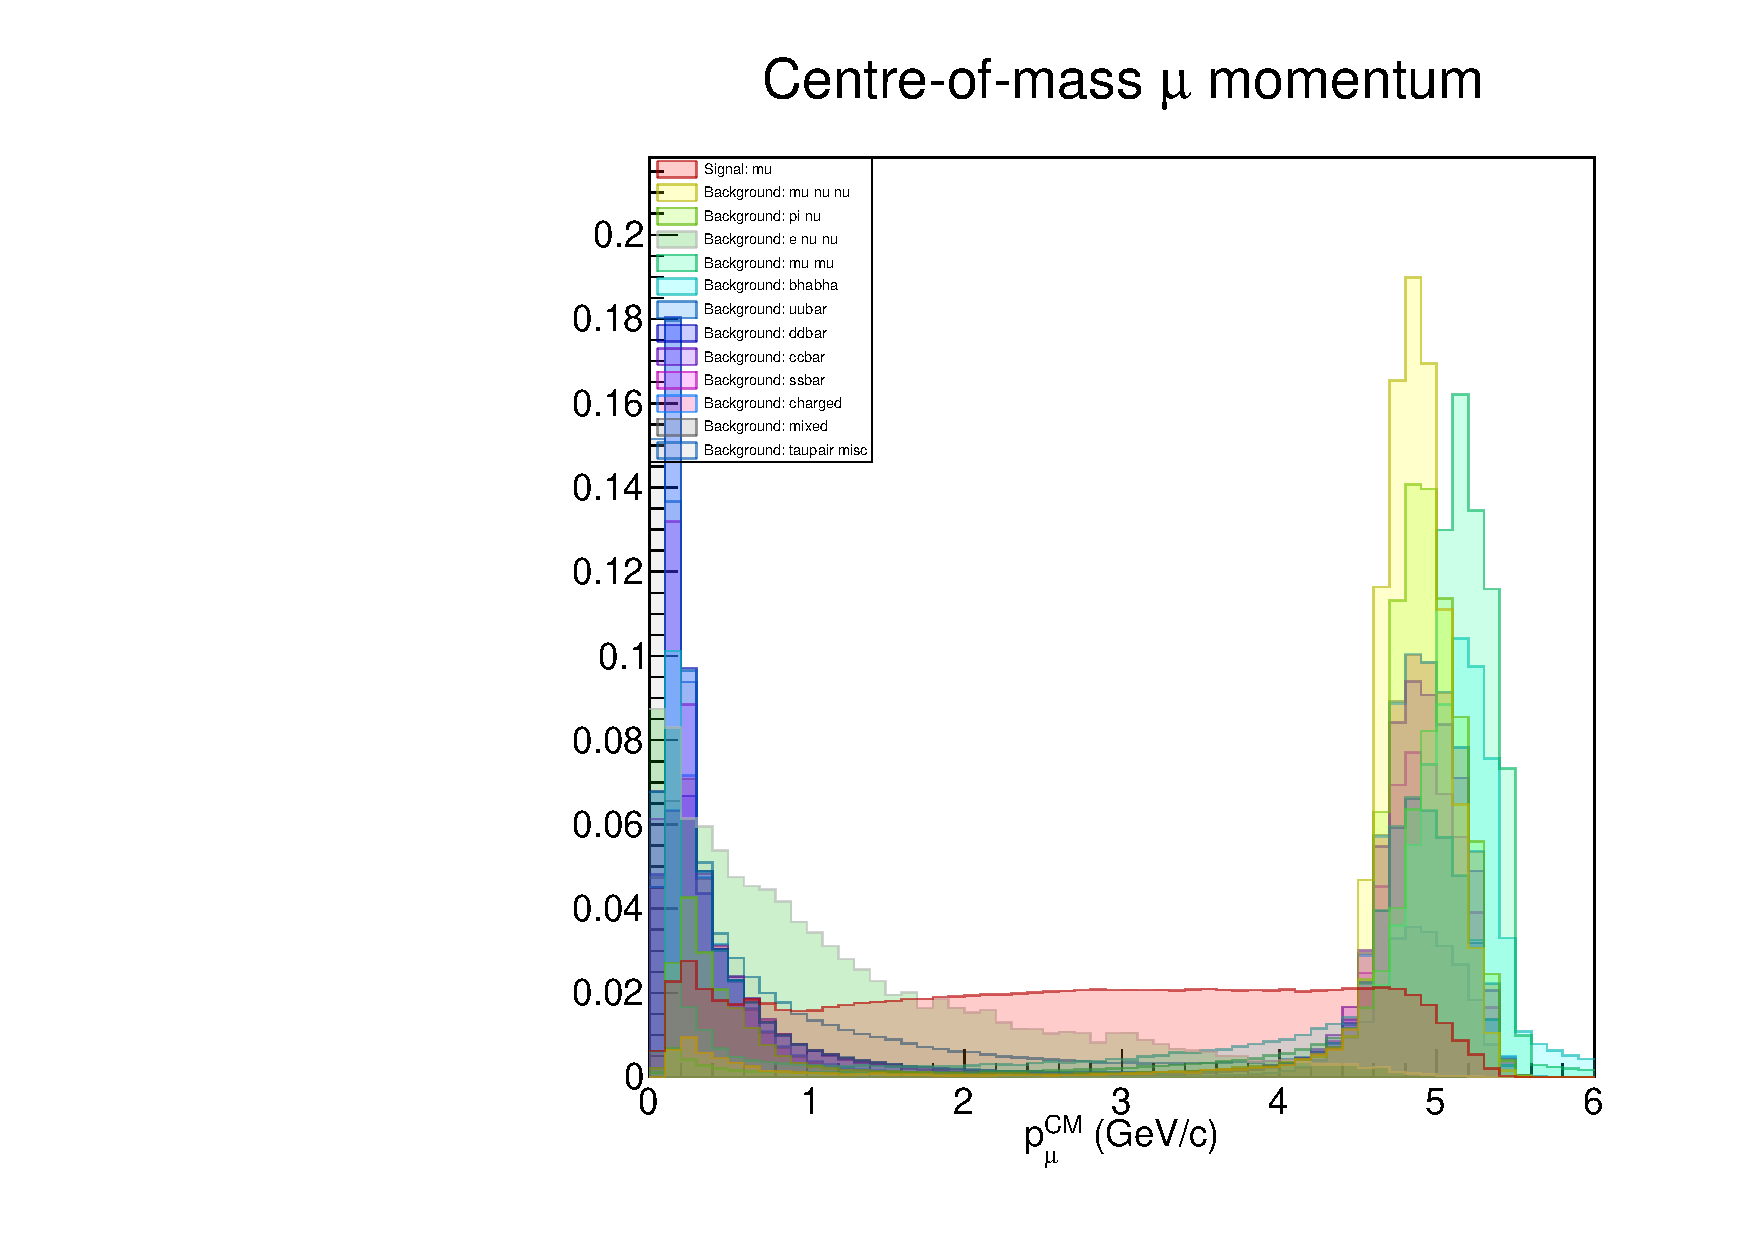
\includegraphics[width=\linewidth]{images/tauMG-muCM_P.pdf}
  \caption[]%
  {{\small Center-of-mass frame momentum of signal muon.}}    
  \label{fig:tauMG muCM P}
\end{minipage}%
        \hfill
\begin{minipage}{.475\textwidth}
  \centering
  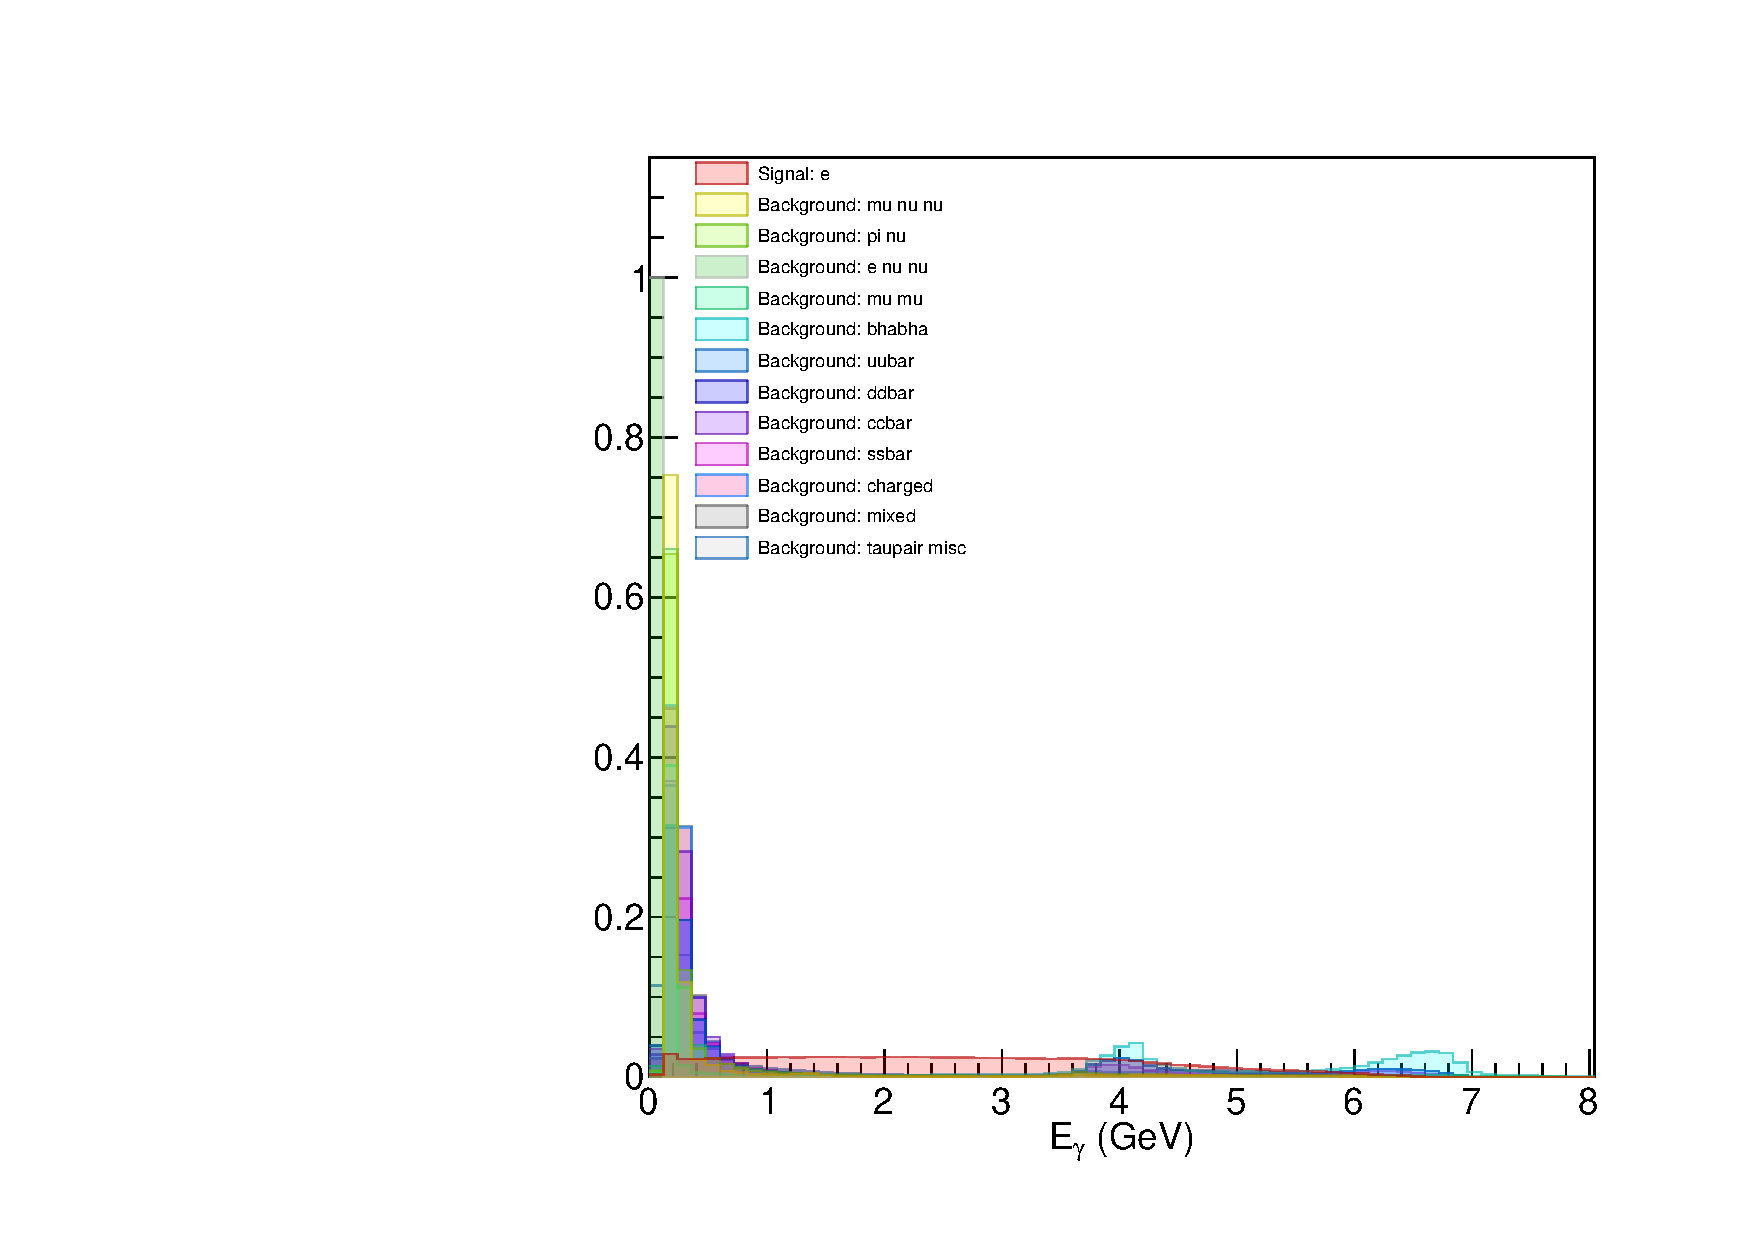
\includegraphics[width=\linewidth]{images/tauMG-gamma_E.pdf}
  \caption[]%
  {{\small Lab frame energy of signal photon.}}  
  \label{fig:tauMG gamma E}
\end{minipage}
        \vskip\baselineskip
\begin{minipage}{.475\textwidth}
  \centering
  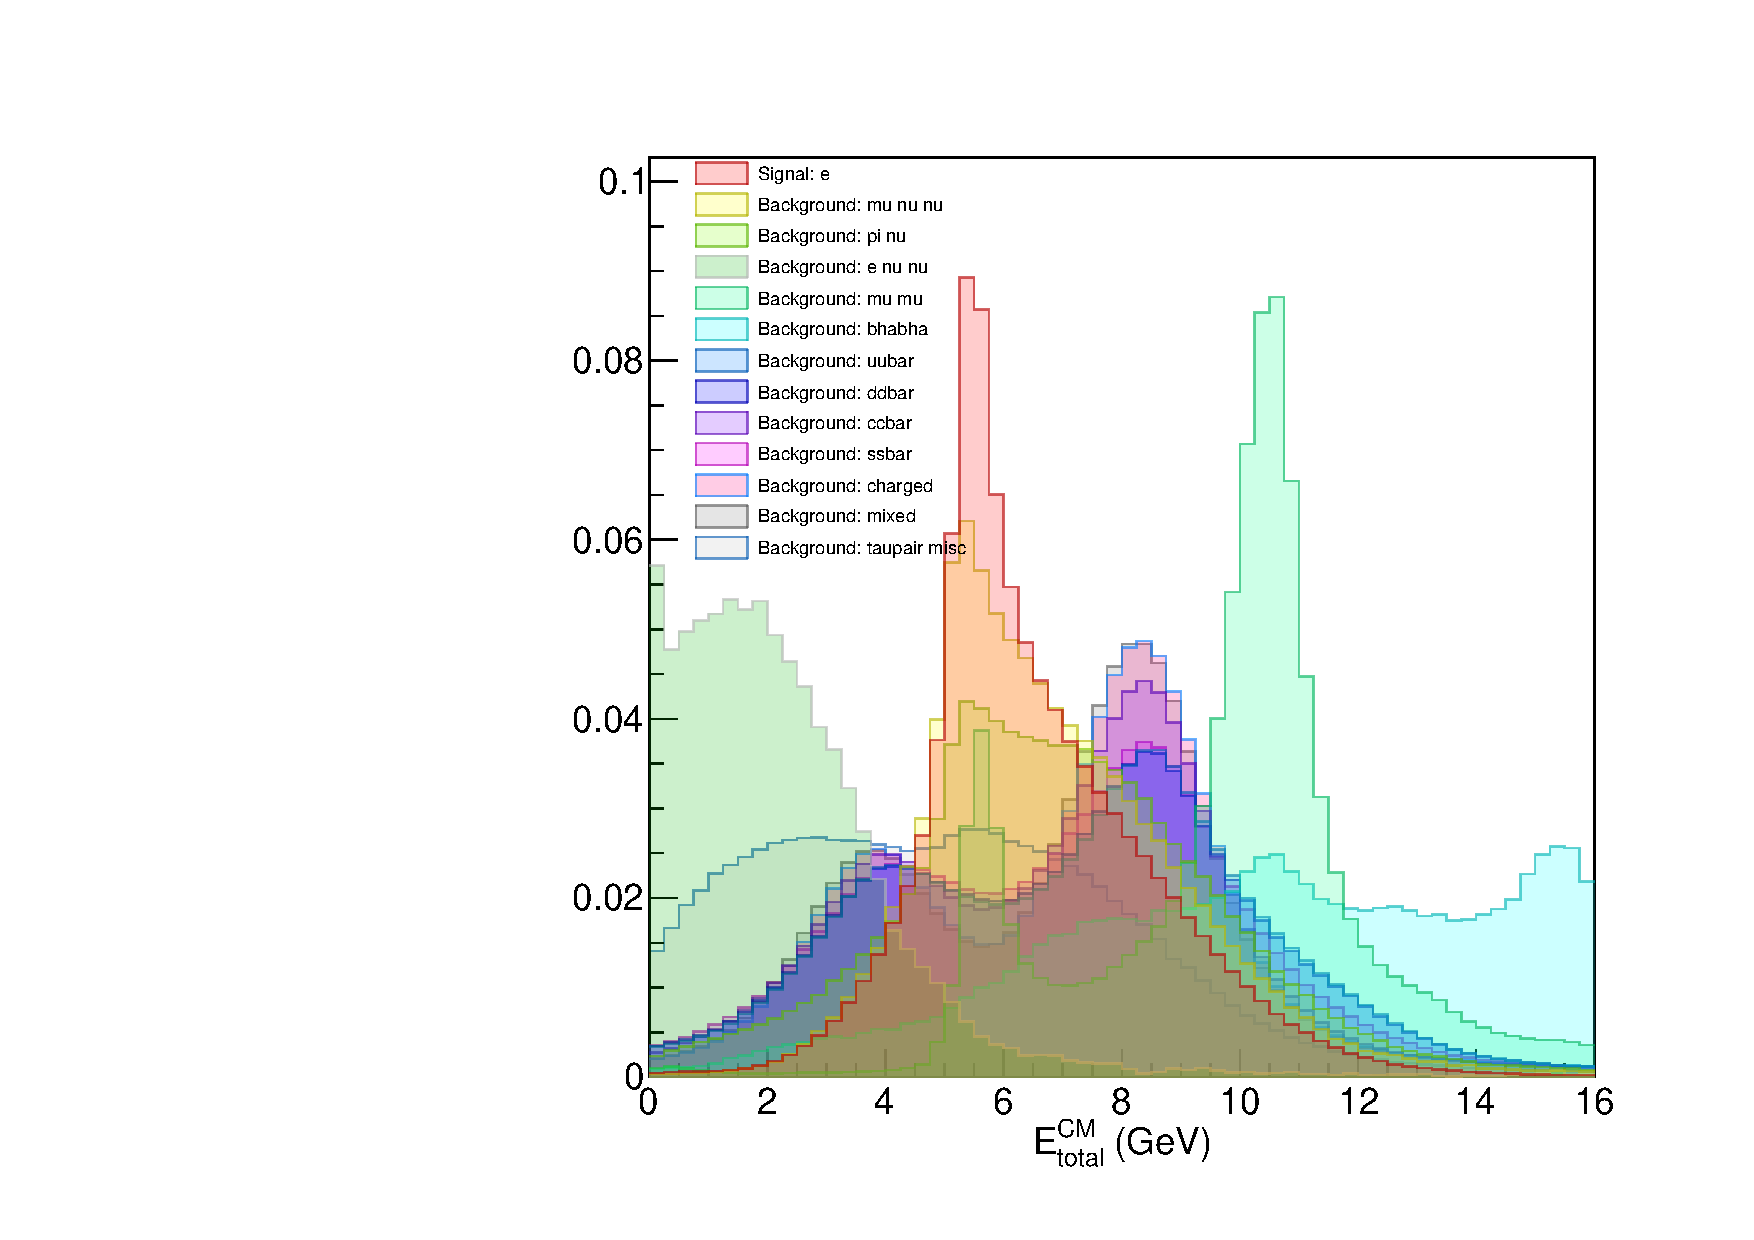
\includegraphics[width=\linewidth]{images/tauMG-totalCM_E.pdf}
  \caption[]%
  {{\small Total center-of-mass energy of the system.}}    
  \label{fig:tauMG EtotalCM}
\end{minipage}%
        \hfill
\begin{minipage}{.475\textwidth}
  \centering
  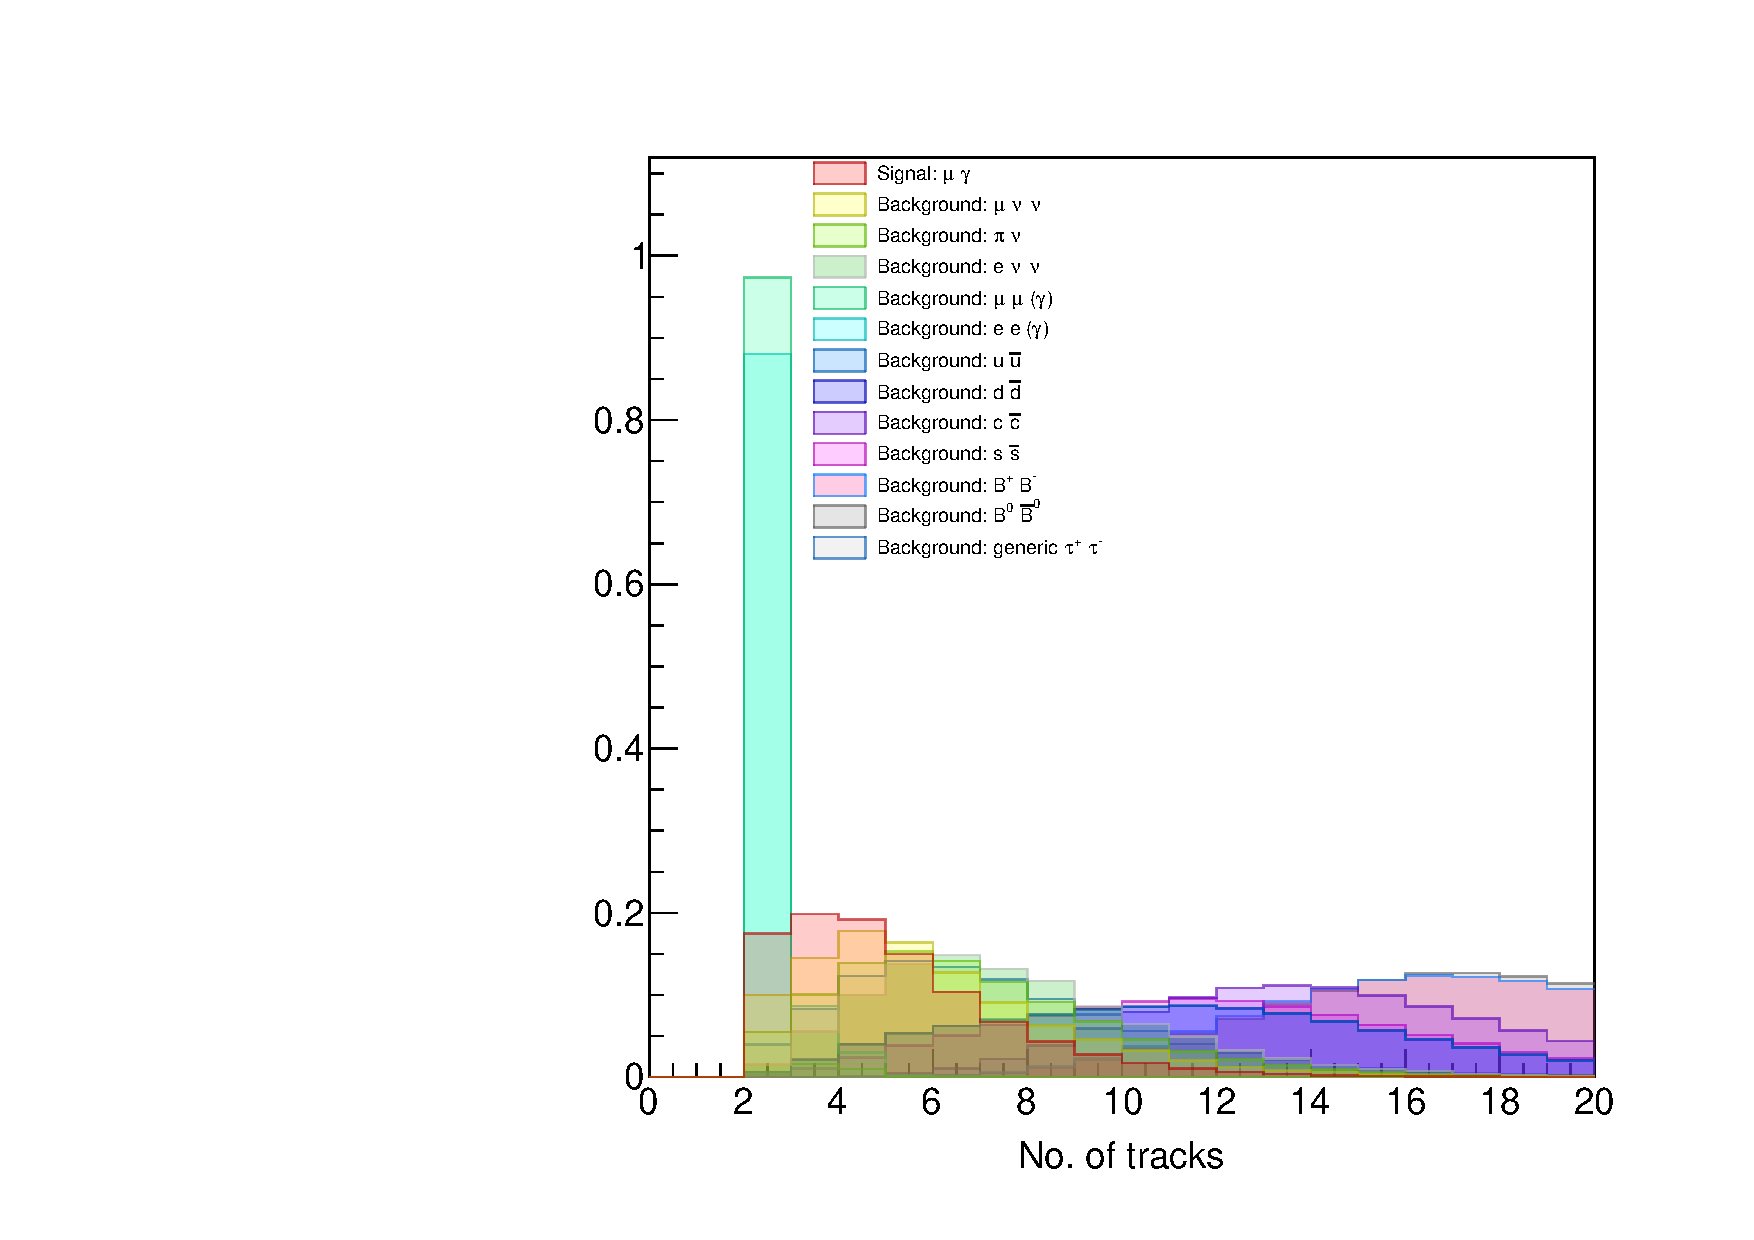
\includegraphics[width=\linewidth]{images/tauMG-tracks.pdf}
  \caption[]%
  {{\small Number of reconstucted tracks.}}  
  \label{fig:tauMG tracks}
\end{minipage}
\end{figure}

\subsection{Electron mode}

Much of the kinematics and topologies as described for the signal muon mode also applies to the signal electron mode. However, it is prudent to note the major difference between the two final state charged particles - specifically the difference in mass. Muons have mass $\SI{105.66}{MeV/c^2}$, over 200 times heavier than electrons, with mass of $\SI{0.511}{MeV/c^2}$. Due to their lighter mass, electrons lose far more energy due to bremsstrahlung (braking radiation). Radiated power from bremsstrahlung goes as $m^{-4}$; electrons lose more energy via bremsstrahlung than muons by factor $\left(m_{\mu}/m_{e}\right)^{4} \sim 200^4$.

Emission of photons due to bremsstrahlung as electrons travel the ECL causes deviations in expected the trajectory of the track, making accurate reconstruction of the signal electron difficult. Due to this energy loss we see a different energy and momentum signature for the signal track compared to the muon mode; peaks for both are located around $\SI{2.5}{GeV}$, but a large fraction of events have energies much lower.

Accurate reconstruction via basf2 is more difficult for these lighter particles, with only a fraction of $\tau\to e\gamma$ events having a reconstructed $\tau$ invariant mass peak anywhere near the $\tau$ mass.


\section{Backgrounds}

\subsection{Tau-pair processes}

A key difference between tau-pair backgrounds and the signal modes investigated is the lack of signal-side photon, and the existence of signal-side neutrinos.

In tau-pair processes, the signal-side $\tau$ of energy $\SI{5.5}{GeV}$ decays dominantly into a single charged track and a neutrino (or neutrinos, in the pion modes). Light neutrinos carry away only a fraction of the energy from its mother particle; we expect the signal track to have a peak in energy of $\approx\SI{5.5}{GeV}$. However, the electron will lose a significant fraction of its energy due to bremsstrahlung as it passes through the detector and hence have a lower average energy. This is consistent with Figure~\ref{fig:tauMG muCM P}.

In most cases for tau-pair processes, the reconstructed signal photon comes from ISR, FSR or more often beam backgrounds. Photons produced as beam background are often low energy, especially compared to the average photon energy from signal processes of $\sim \SI{2.25}{GeV}$. Signal photon energy is shown in Figure~\ref{fig:tauMG muCM P}; we note the peak energy of $E_{\gamma}<\SI{1}{GeV}$ for tau-pair processes. 

Since the signal photon does not originate from the signal-side $\tau$, the signal tracks appears ``boosted'' by comparison. This boost leads to the signal track and signal photon travelling almost back-to-back in the center-of-mass frame, in contrast to the signal mode where these final state particles have only a small opening angle between them (see Figure~\ref{fig:taupair muGammaOpeningCosThetaCM}). 

\begin{figure}
\centering
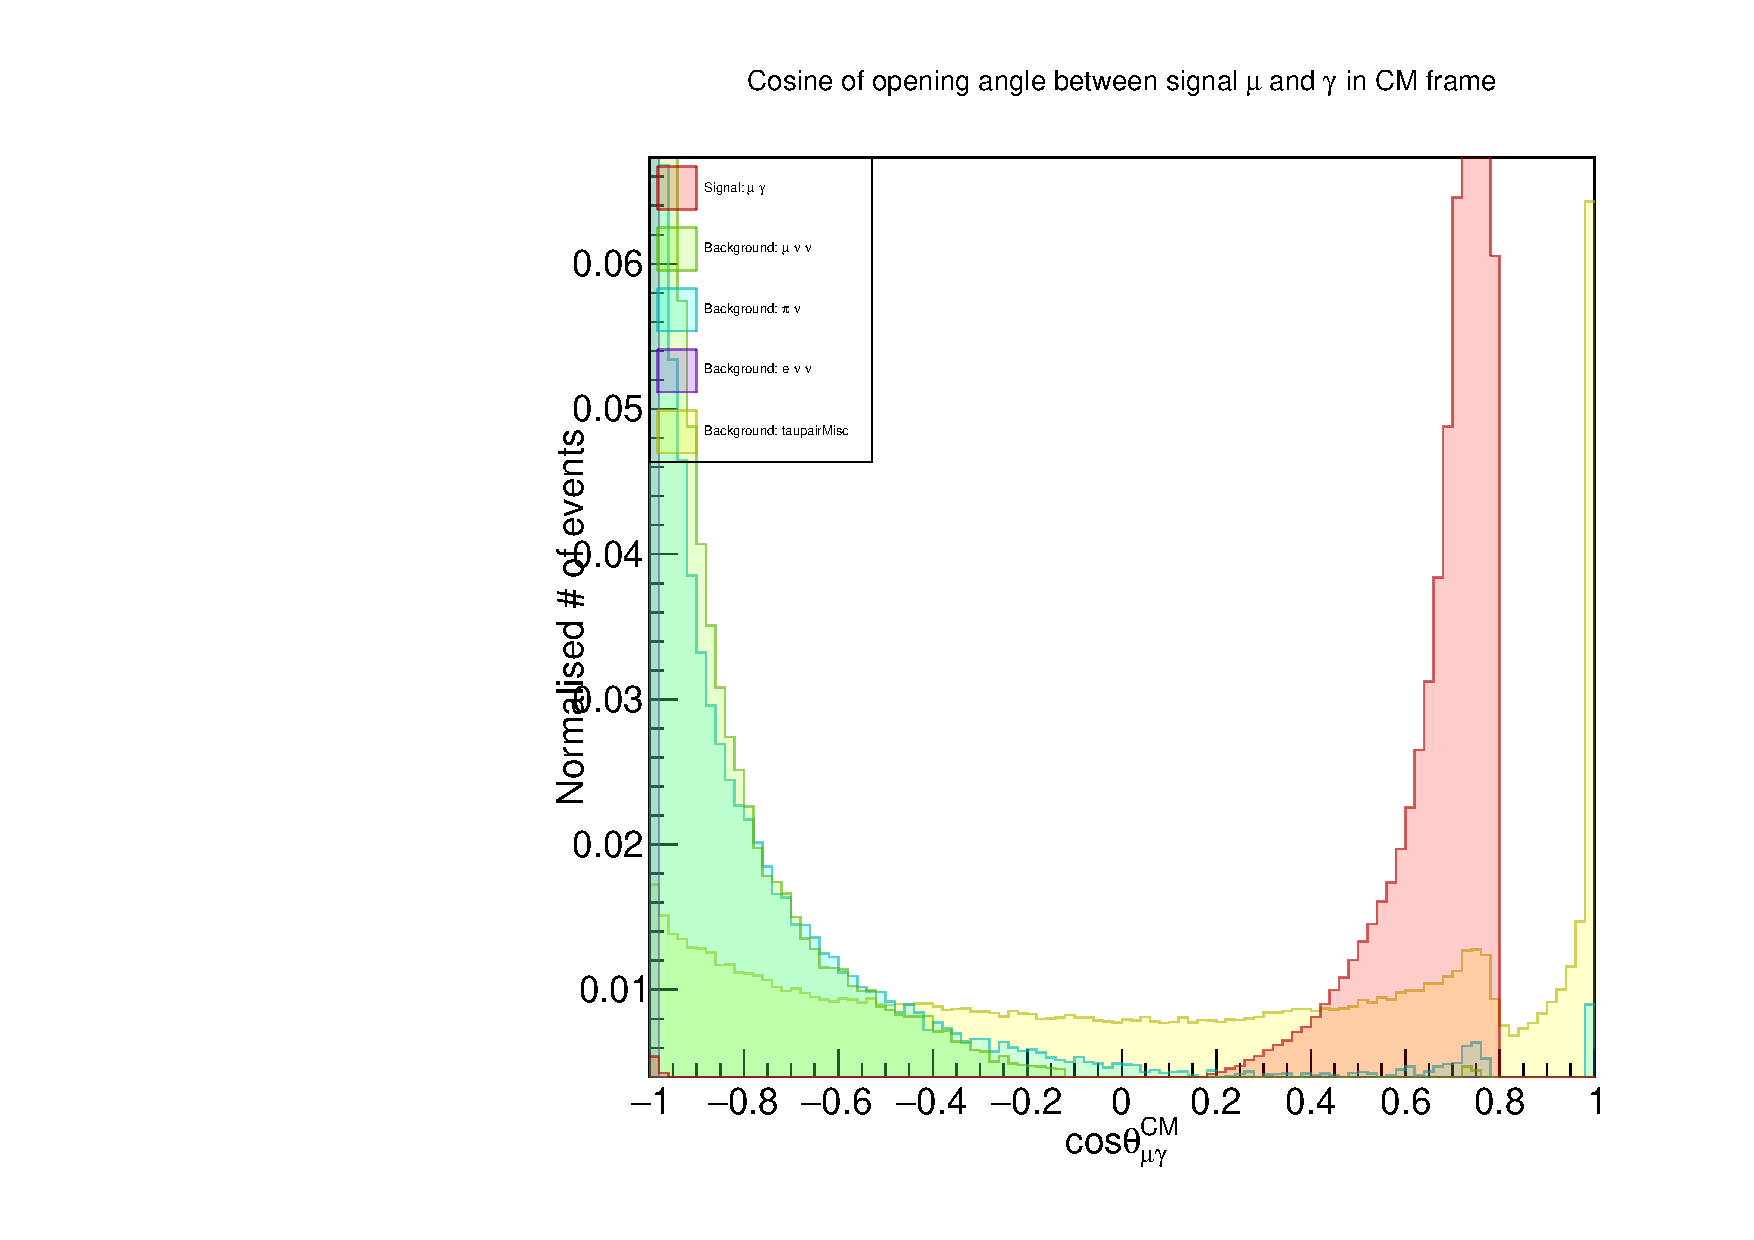
\includegraphics[width=0.45\linewidth]{images/taupair-muGammaOpeningCM.pdf}
\caption[]%
{{\small Cosine of the opening angle between signal track and signal photon in the center-of-mass frame; comparison between $\tau\to\mu\gamma$ and background tau-pair processes.}}    
\label{fig:taupair muGammaOpeningCosThetaCM}
\end{figure}


\subsection{Mu-pair processes}

Muons are very cleanly reconstructed by the detector; they do not lose any significant amount of energy through bremsstrahlung radiation, and they penetrate deeply leaving a distinct signal. Unlike the tau-pair processes or the signal modes discussed above, mu-pair processes $e^+ e^- \to \mu^+ \mu^- (\gamma)$, both signal- and tag-side channels consist of only a single charged track each, sometimes with a final state photon. Hence, mu-pair processes are reconstructed very well. This is evidenced by the majority of events with only two reconstructed tracks; this is is stark comparison to the spread of tracks from two up to fifteen in tau-pair events. Total reconstructed energy peaks around $\SI{10.5}{GeV}$.

By momentum conservation, the signal and tag tracks are generated back-to-back for $\mu\mu$ final states, or with an opening angle similar to the signal mode for radiative $\mu\mu\gamma$ final states. The signal photon is often reconstructed from low energy beam background photons, as with background tau-pair processes. A similar photon energy spectrum can be seen in Figure~\ref{fig:tauMG gamma E}.

\subsection{Bhabha}

Bhabha events $e^+ e^- \to e^+ e^- (\gamma)$ have similar event signatures to mu-pair processes $e^+ e^- \to \mu^+ \mu^- (\gamma)$ across a range of variables, for obvious reasons. However, as is case with electrons in the detector, both signal- and tag-track particles lose a significant portion of their energy to bremsstrahlung and are not reconstructed as cleanly as muons. 

Smearing of energies and momenta occurs for Bhabha event reconstruction, with measureables not peaking as strongly as for mu-pair events and instead spreading across a values. These features are shown in Figures~\ref{fig:bhabha mupair muCM P} and~\ref{fig:bhabha mupair EtotalCM} below, comparing distributions for mu-pair events to bhabha events. Much of the event topology is still common between these processes, however.

\begin{figure}[h]
\centering
\begin{minipage}{.475\textwidth}
  \centering
  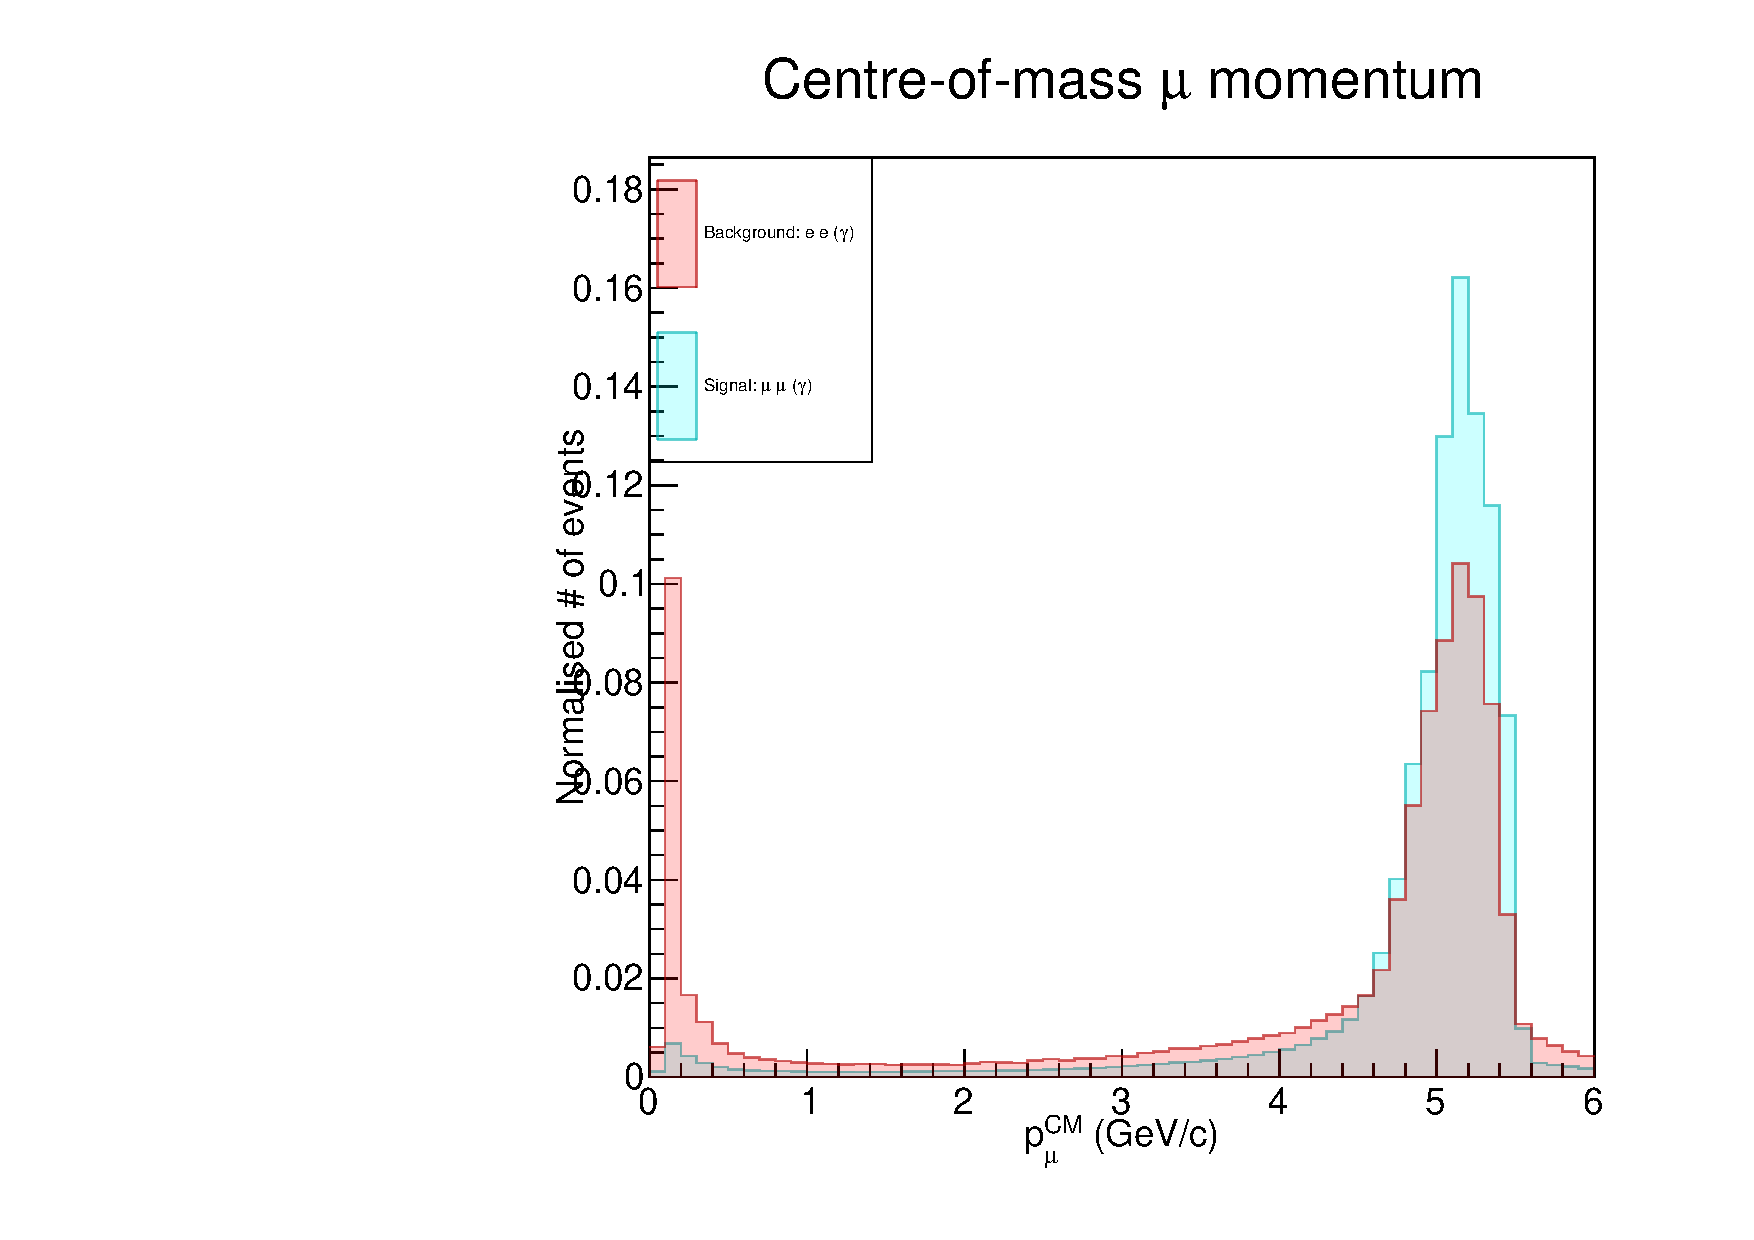
\includegraphics[width=\linewidth]{images/bhabha-mupair-muCM_P.pdf}
  \caption[]%
  {\small Comparison of center-of-mass frame signal track momentum for Bhabha and mu-pair events.}
  \label{fig:bhabha mupair muCM P}
\end{minipage}%
\hfill
\begin{minipage}{.475\textwidth}
  \centering
  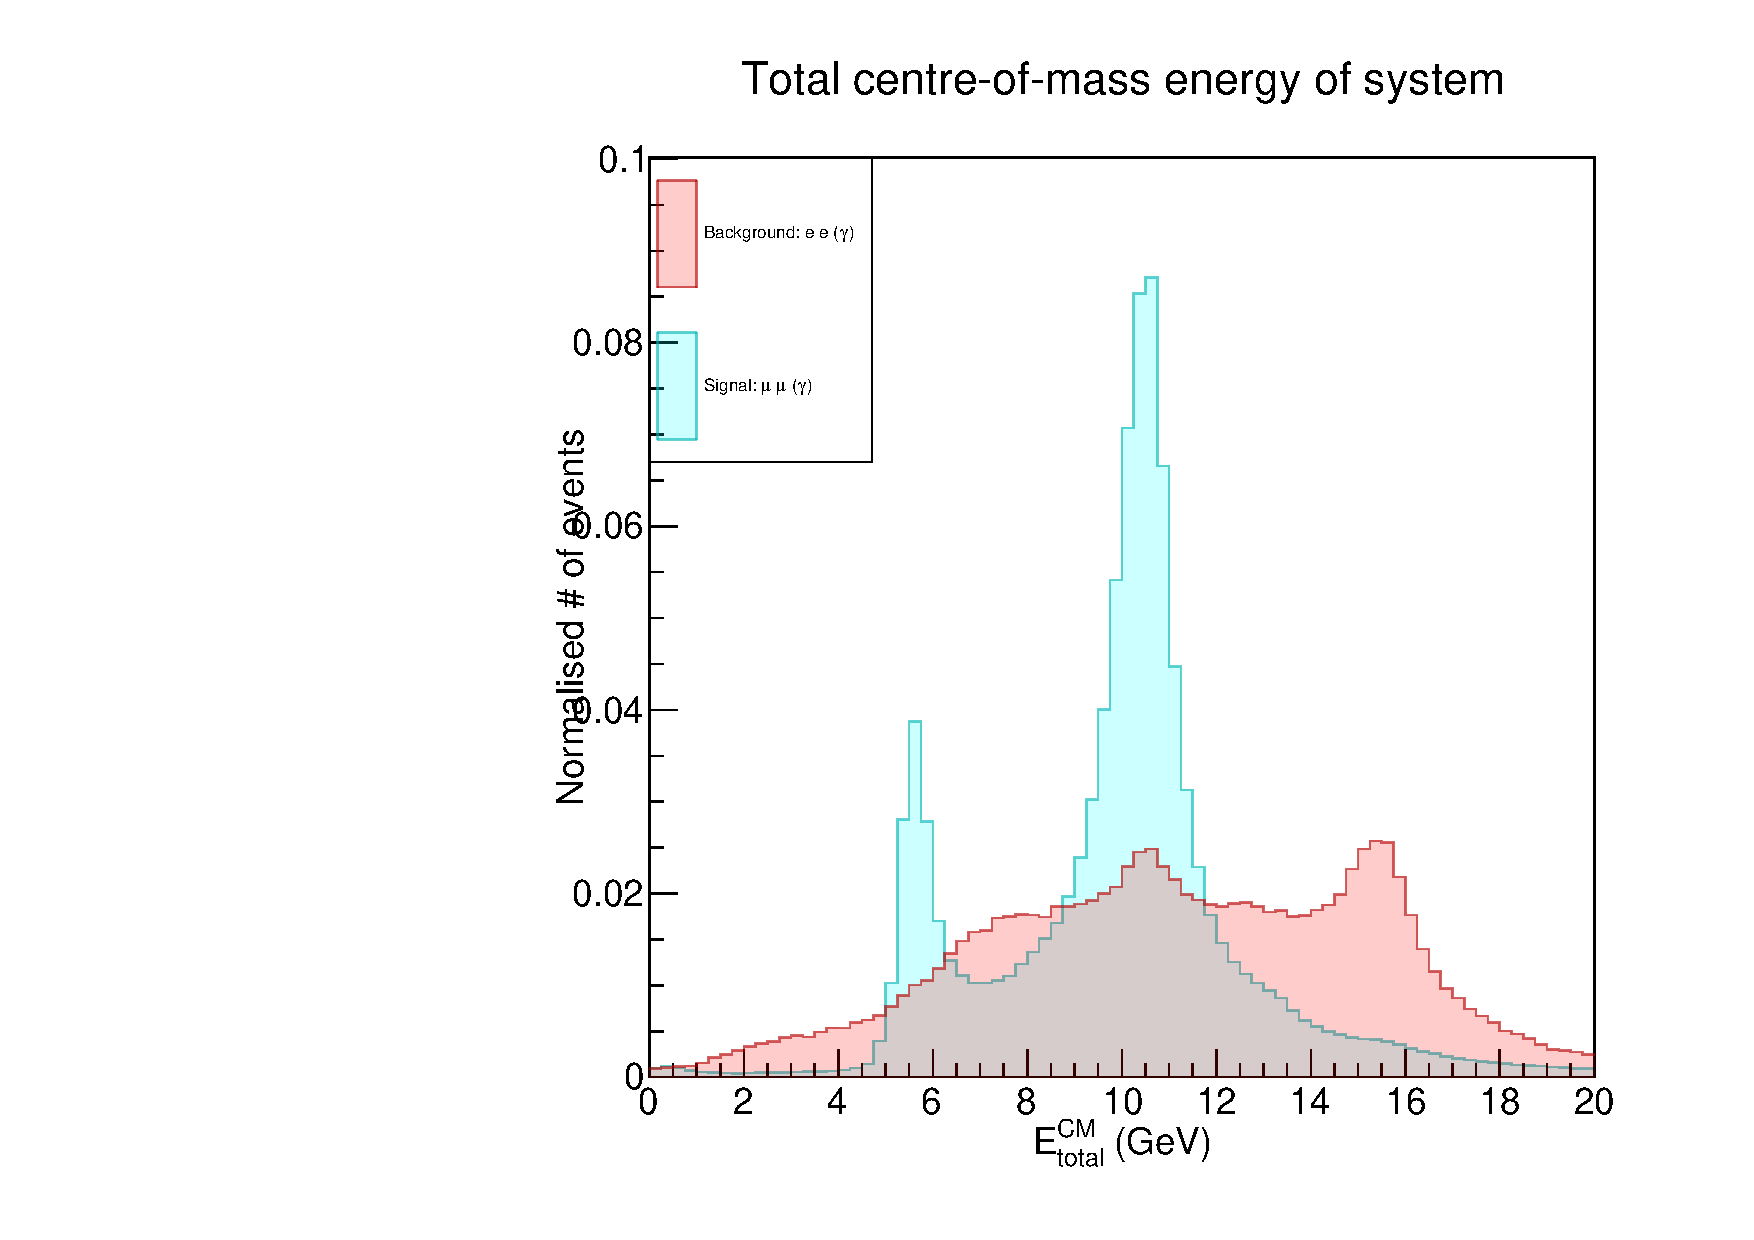
\includegraphics[width=\linewidth]{images/bhabha-mupair-totalCM_E.pdf}
  \caption[]%
  {\small Comparison of total energy of the system in center-of-mass frame for Bhabha and mu-pair events.}
  \label{fig:bhabha mupair EtotalCM}
\end{minipage}
\end{figure}


\subsection{Continuum and $B\bar{B}$}

Hadronic backgrounds at Belle II come from the events $e^+ e^- \to q\bar{q}$ and $e^+ e^- \to B \bar{B}$. The event rate for the energies at which we investigate is dominated by these processes, however their event signatures are distinct from leptonic processes in many variables allowing good separation. 

\begin{figure}[h]
\centering
  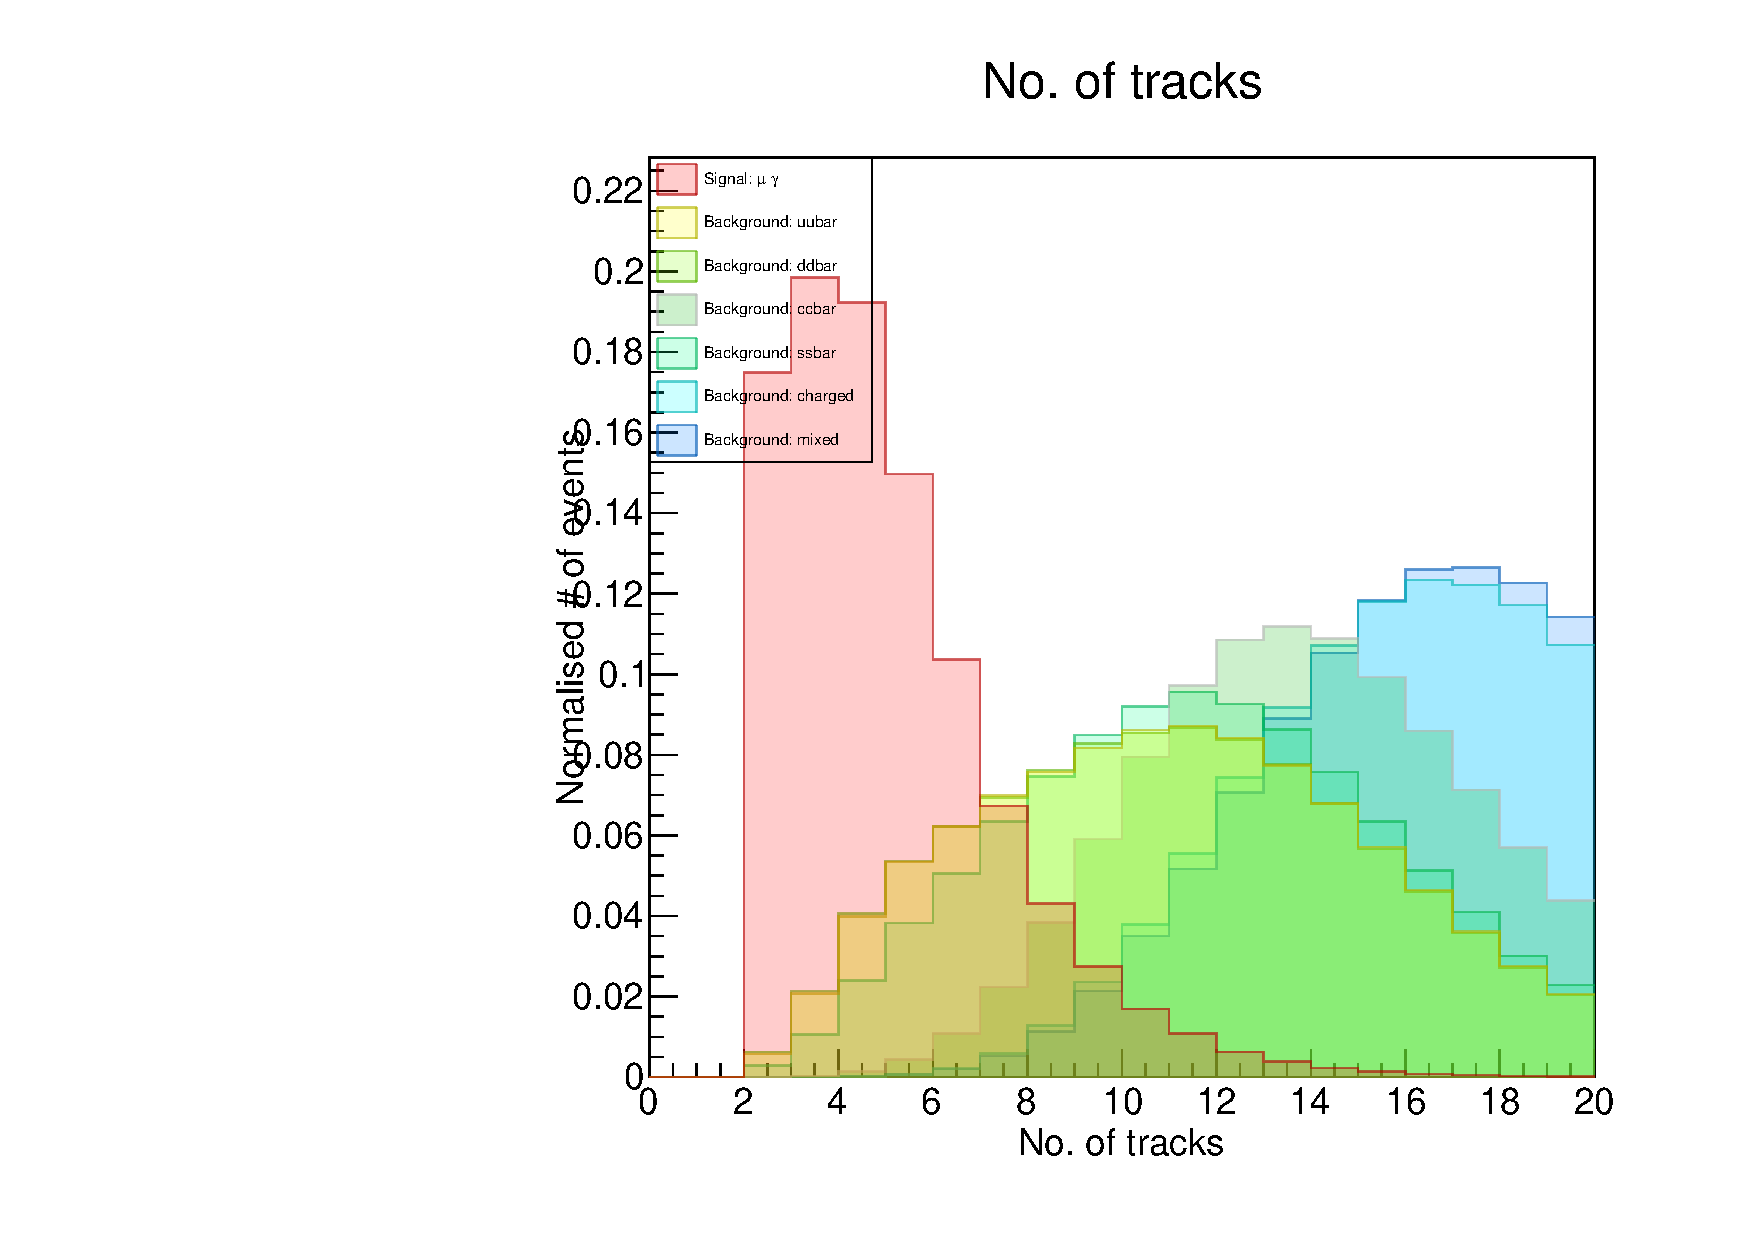
\includegraphics[width=0.5\linewidth]{images/hadronic-tracks.pdf}
  \caption[]%
  {\small Number of tracks in continuum and $B\bar{B}$ events.}
  \label{fig:hadronic tracks}
\end{figure}

\pagebreak

%-------------------------------------------------------------------

\chapter{Preselection}

Following reconstruction, preselection criteria were applied to the reconstructed events. Preselection criteria are defined as distinct from selection criteria in that they remove a minimal amount of signal while removing the more obvious background components; in choosing selection criteria we seek to maximise $S/\sqrt{S+B}$, which may necessarily involve the exclusion of a non-negligible amount of signal.

The preselection criteria were selected by inspection of plots of various topology and energy based variables. Different preselection and selection criteria are chosen for each final state mode, due to the different event signatures. A total of 5 variables where chosen for preselection.

\section{Muon mode}

Specific values for preselection are listed in Table~\ref{tab:preselection cuts muon mode}. Signal and background efficiencies after preselection are shown in Table~\ref{tab:preselection events muon mode}.

98.06\% of reconstructed $\tau\to\mu\gamma$ signal events pass the preselection criteria; around 1,000,000,000 background events out of 2,000,000,000 are removed through this process. 

\begin{table}[h]
\centering
\begin{tabular}{llll}
\textbf{symbolic} & \textbf{description} & \textbf{lower} & \textbf{upper} \\ \hline
$p_{\text{tag}}^{\text{CM}}$  & CM momentum of tag track & --- & $\SI{5.2}{GeV}$ \\
$\cos\theta_{\text{signal}}$ & Cosine of polar angle of signal track & $-0.9$ & --- \\
$E_{\text{total}}^{\text{CM}}$ & Center-of-mass energy of total system  & --- & $\SI{15}{GeV}$ \\
$\lvert\text{thrust}\rvert$ & Magnitude of signal thrust vector* & 0.92 & --- \\
$E_{\text{sum}}^{\text{CM}}$ & Center-of-mass energy of photons and tracks & $\SI{4.5}{GeV}$ & ---
\end{tabular}
\caption{Preselection cuts (muon mode)}
\label{tab:preselection cuts muon mode}
\end{table}

We also place a loose requirement of $M_{\text{inv}}$, requiring $1.65 < M_{\text{inv}} < 1.85$. Although this is one of our signal region variables, we are justfied in applying loose preselection on it because events outside this selection will lie outside the final signal region, and hence be unimportant to the analysis.

\begin{table}[h]
\centering
\begin{tabular}{lrrc}
\textbf{MC type}         & \textbf{events in (scaled)} & \textbf{events out} & $\mathbf{\epsilon_{\text{ps}}}$ \\ \hline 
\rowcolor[HTML]{EFEFEF} 
$\tau\to\mu\gamma$       & \num{140}        & \num{135}      & $\SI{96.32}{\percent}$                   \\
$\tau\to\mu\nu\nu$      & \num{678130}         & \num{631235}          & $\SI{93.08}{\percent}$           \\
$\tau\to\pi\nu$         & \num{1076758}       & \num{822028}          & $\SI{76.34}{\percent}$            \\
$\tau\to e\nu\nu$       & \num{109810}        & \num{70675}         & $\SI{64.36}{\percent}$      \\
$\tau\to\text{generic}$  & \num{2304225}       & \num{636954}          & $\SI{27.64}{\percent}$         \\
$e^+ e^- \to \mu^+ \mu^- (\gamma)$   & \num{39857811}    & \num{21938180}     & $\SI{55.04}{\percent}$   \\
$e^+ e^- \to e^+ e^- (\gamma)$      & \num{7111247601}      & \num{1457005758}       & $\SI{20.49}{\percent}$     \\
$e^+ e^- \to u \bar{u}$       & \num{66447114}           & \num{29767142}  & $\SI{44.80}{\percent}$ \\
$e^+ e^- \to d \bar{d}$        & \num{16384978}       & \num{7307320}      & $\SI{44.60}{\percent}$       \\
$e^+ e^- \to c \bar{c}$        & \num{6017200}       & \num{23401910}           & $\SI{38.99}{\percent}$          \\
$e^+ e^- \to s \bar{s}$       & \num{14579500}     & \num{6299797}            & $\SI{43.21}{\percent}$         \\
$e^+ e^- \to B^+ B^-$     & \num{56664730}       & \num{22083348}           & $\SI{38.97}{\percent}$          \\
$e^+ e^- \to B^0 \bar{B}^0$       & \num{60329511}           & \num{23372366}        & $\SI{61.26}{\percent}$              
\end{tabular}
\caption{Preselection efficiency (muon mode).}
\label{tab:preselection events muon mode}
\end{table}


\section{Electron mode}

Separate preselection criteria was chosen for the electron mode. These criteria do not differ much, as expected, however due to the prevalence of bremsstrahlung in the electron mode the energy variables differ greatly. Due to this we set an upper limit on $E^{\text{CM}}_{\text{sum}}$ rather than a lower limit as for the muon mode.

\begin{table}[h]
\centering
\begin{tabular}{llll}
\textbf{symbolic} & \textbf{description} & \textbf{lower} & \textbf{upper} \\ \hline
$p_{\text{tag}}^{\text{CM}}$  & CM momentum of tag track & --- & $\SI{5}{GeV}$ \\
$\cos\theta_{\text{signal}}$ & Cosine of polar angle of signal track & $-0.975$ & --- \\
$E_{\text{total}}^{\text{CM}}$ & Center-of-mass energy of total system  & --- & $\SI{14}{GeV}$ \\
$\lvert\text{thrust}\rvert$ & Magnitude of signal thrust vector* & 0.92 & --- \\
$E_{\text{sum}}^{\text{CM}}$ & Center-of-mass energy of photons and tracks & $\SI{4.5}{GeV}$ & ---
\end{tabular}
\caption{Preselection cuts (electron mode)}
\label{tab:preselection cuts electron mode}
\end{table}

\begin{table}[h]
\centering
\begin{tabular}{lrrc}
\textbf{MC type}         & \textbf{events in (scaled)} & \textbf{events out} & $\mathbf{\epsilon_{\text{ps}}}$ \\ \hline 
\rowcolor[HTML]{EFEFEF} 
\end{tabular}
\caption{Preselection efficiency (electron mode).}
\label{tab:preselection events electron mode}
\end{table}

Again, a loose requirement of $1.65 < M_{\text{inv}} < 1.85$ is required for event preselection. The preselection event information for the electron mode is given in Table~\ref{tab:preselection events electron mode}. We note the dramatic drop in the number of $\tau\to e\gamma$ signal events. This is due to the restriction of $M_{\text{inv}}$. We expect a peak around the invariant mass of the $\tau$, $m_{\tau}\sim \SI{1.777}{GeV/c^2}$; see Figure~\ref{fig:tauMG tauMG tauinvmass}. For the electron mode a peak occurs slightly after that mass, around $\SI{1.8}{GeV/c^2}$. More important, however, is the high multiplicity of events at $M_{\text{inv}}=0$. Obviously this is an unphysical value --- we determine that this feature is due to the large number of signal electron tracks which are not reconstructed properly.

\begin{figure}
\centering
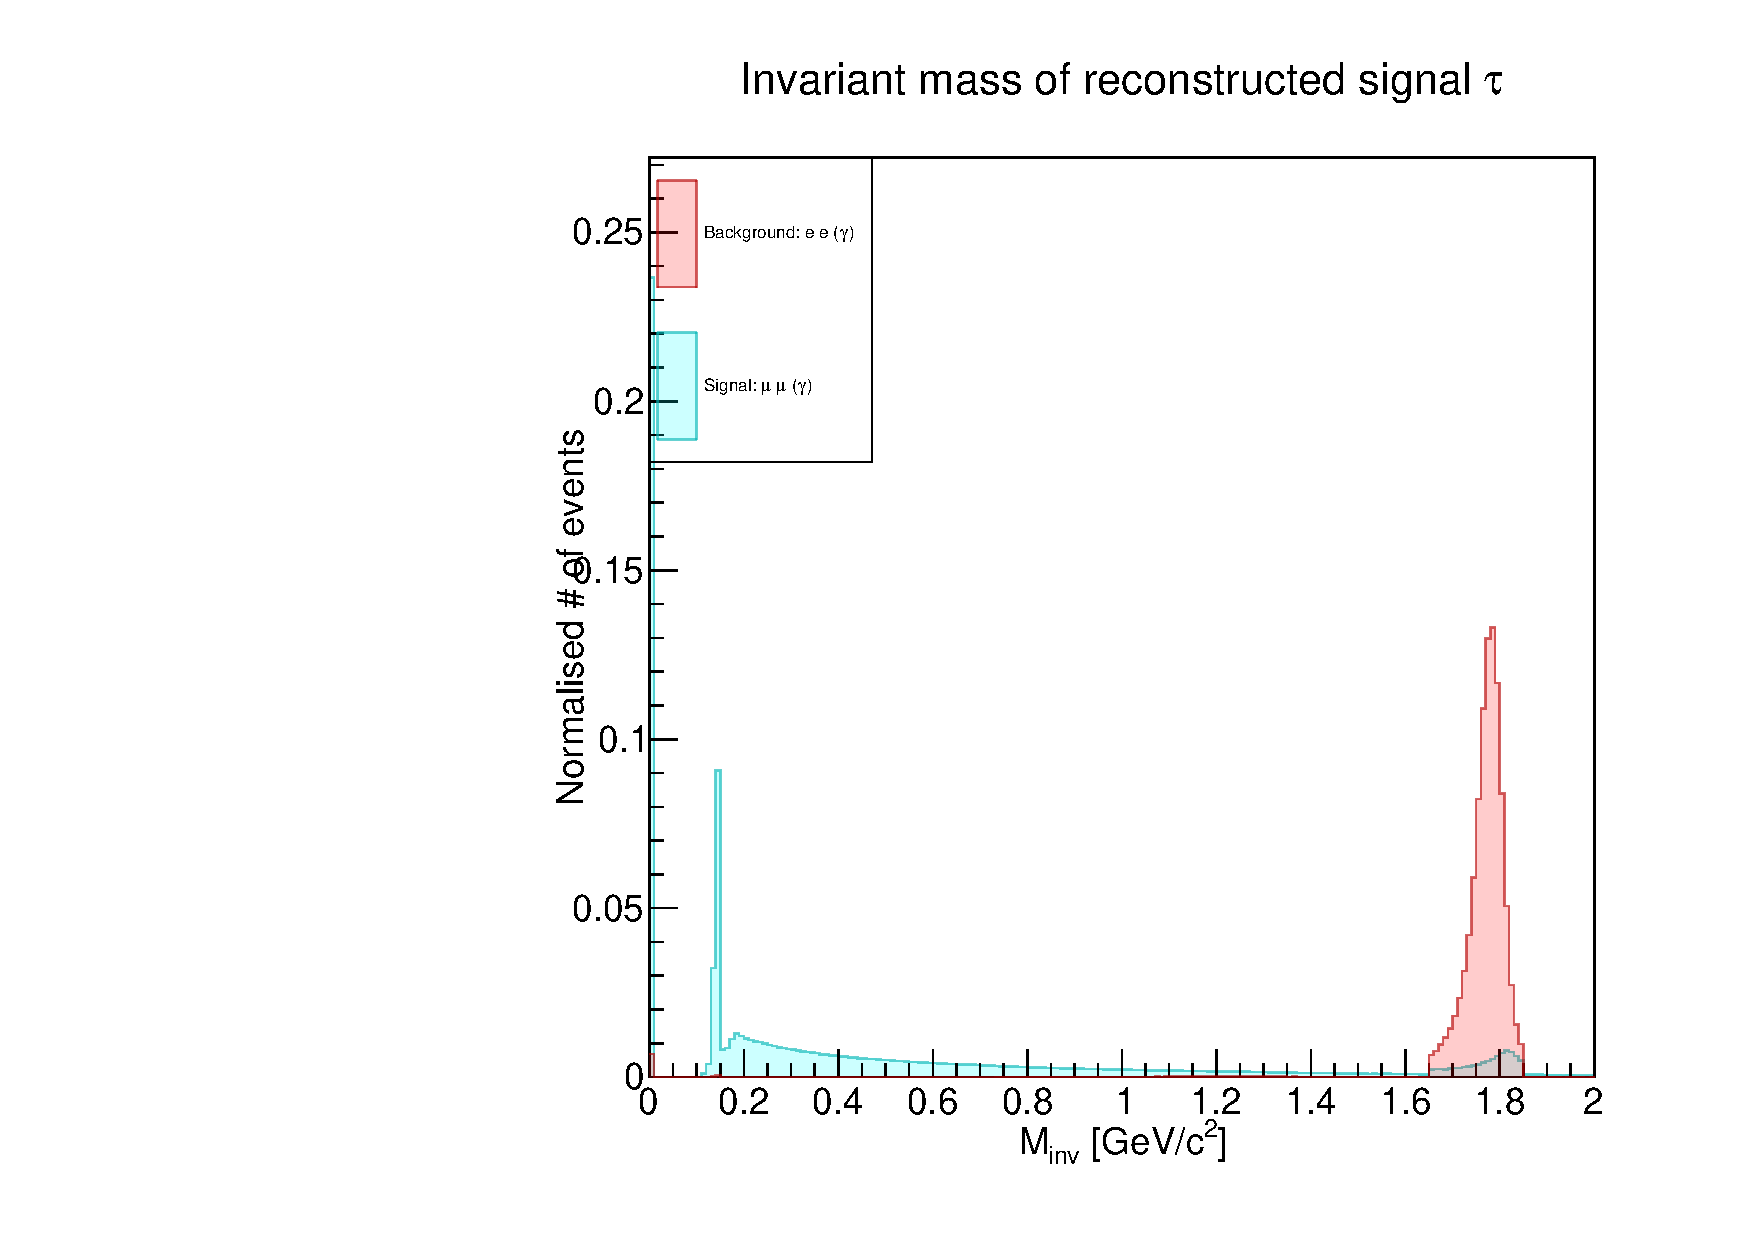
\includegraphics[width=0.6\linewidth]{images/tauMG-tauEG-tauinvmass.pdf}
\caption[]%
{{\small Comparison of $M_{\text{inv}}$ for signal muon and signal electron modes. Note that we expect a peak around $m_{\tau}\sim \SI{1.777}{GeV/c^2}$.}}
\label{fig:tauMG tauMG tauinvmass}
\end{figure}

After preselection, the signal electron mode has an efficiency of only $\SI{9.95}{\percent}$. The total efficiency of the signal muon mode after all selection criteria have been applied (Section XXXXX) is, in comparison, $\SI{7.23}{\percent}$ - we would expect that the efficiency of the electron mode would get considerably worse after event selection. Due to this poor reconstruction and minimal number of events remaining only after preselection, we do not continue to full event selection in MC for $\tau\to e\gamma$. Unless otherwise specified, the remainder of the analysis will concern the mode $\tau\to\mu\gamma$ only.


\pagebreak

%-------------------------------------------------------------------

\begin{comment}
\chapter{Correlation}

The final signal region in which events will be selected from lies in $\Delta E$ vs. $M_{\text{inv}}$ space. To avoid biasing event selection, only loose cuts are applied to these variables throughout. We also investigate the correlation between these signal variables and other variables which we may cut over, to avoid introducing bias through these correlations. 

???

\pagebreak
\end{comment}

%-------------------------------------------------------------------

\chapter{Signal optimisation}

There are many reasonable ways to quantify signal optimisation compared to background in a particle physics analysis. For this analysis, we have chosen the measure of signal optimisation $S/\sqrt{S+B}$. $S$ is the expected number of signal events remaining after event selection has been performed; note that we scale for our signal events dependent on their associated LFV branching fractions, which are currently experimental upper bounds. Hence the measure $S/\sqrt{S+B}$ will vary for different branching fraction hypotheses. 
Similarly $B$ is the expected number of background events remaining after event selection; specifically this is the sum of all events remaining across all background MC used in analysis. Since not all possible background processes have been included we would expect the empirical value of $B$ to be higher; this is mostly unimportant for our analysis since we need only compare changes in $S/\sqrt{S+B}$ between different selection criteria, not to know the absolute value.

To maximise $S/\sqrt{S+B}$, the number of background events must be reduced while not removing too many sgnal events. This is especially important given the low branching fraction of our signal - taking the experimental upper limit of the $\tau\to\mu\gamma$ branching fraction, we expect only 83 signal events, after reconstruction and preselection, in a $\SI{1}{ab^{-1}}$ dataset, compared to over \num{1500000000} (1.5 billion) background events in the same luminosity.

Forty selection criteria were used in selecting for $\tau\to\mu\gamma$ events. Some variables were taken from the previous search for $\tau\to\ell\gamma$ at Belle (REF); more were added as the analysis progressed to achieve better greater signal separation. Some of these variables were not included in the final analysis. Notable were those related to missing momentum and mass, as some uncertainty was held regardly the accurate reconstruction of these variables. Others such as tag-track transverse momentum and signal-track momentum were not included due to significant overlap of background exclusion with other variables (most obviously center-of-mass tag track momentum and center-of-mass signal-track momentum) causing selection on these measureables to have little to no impact on signal optimisation.
The thresholds were chosen via a manually iterative process, continually improving the ratio $S/\sqrt{S+B}$ by adding or refining criteria. Initial criteria were informed by a combination of automatic iteration over a range of threshold values for around 20 variables, and by visual inspection. As this is the first $\tau$ study performed at Belle II, we are justified in selecting some criteria through inspection of plots as it serves as validation of the reconstruction process.

The accomplish the former, selection was repeatedly performed over all MC with only a single criteria applied. The lower or upper threshold of this criteria was modified by a small increment each time. The resulting value of $S/\sqrt{S+B}$ was then plotted against the selection threshold; this plot is called a figure-of-merit plot. An obvious peak, as in Figure~\ref{fig:fom plot muCM P}, indicates a useful value for selection. For many variables, no peak was apparent and so no initial threshold could be chosen through this method.

\begin{figure}[h]
\centering
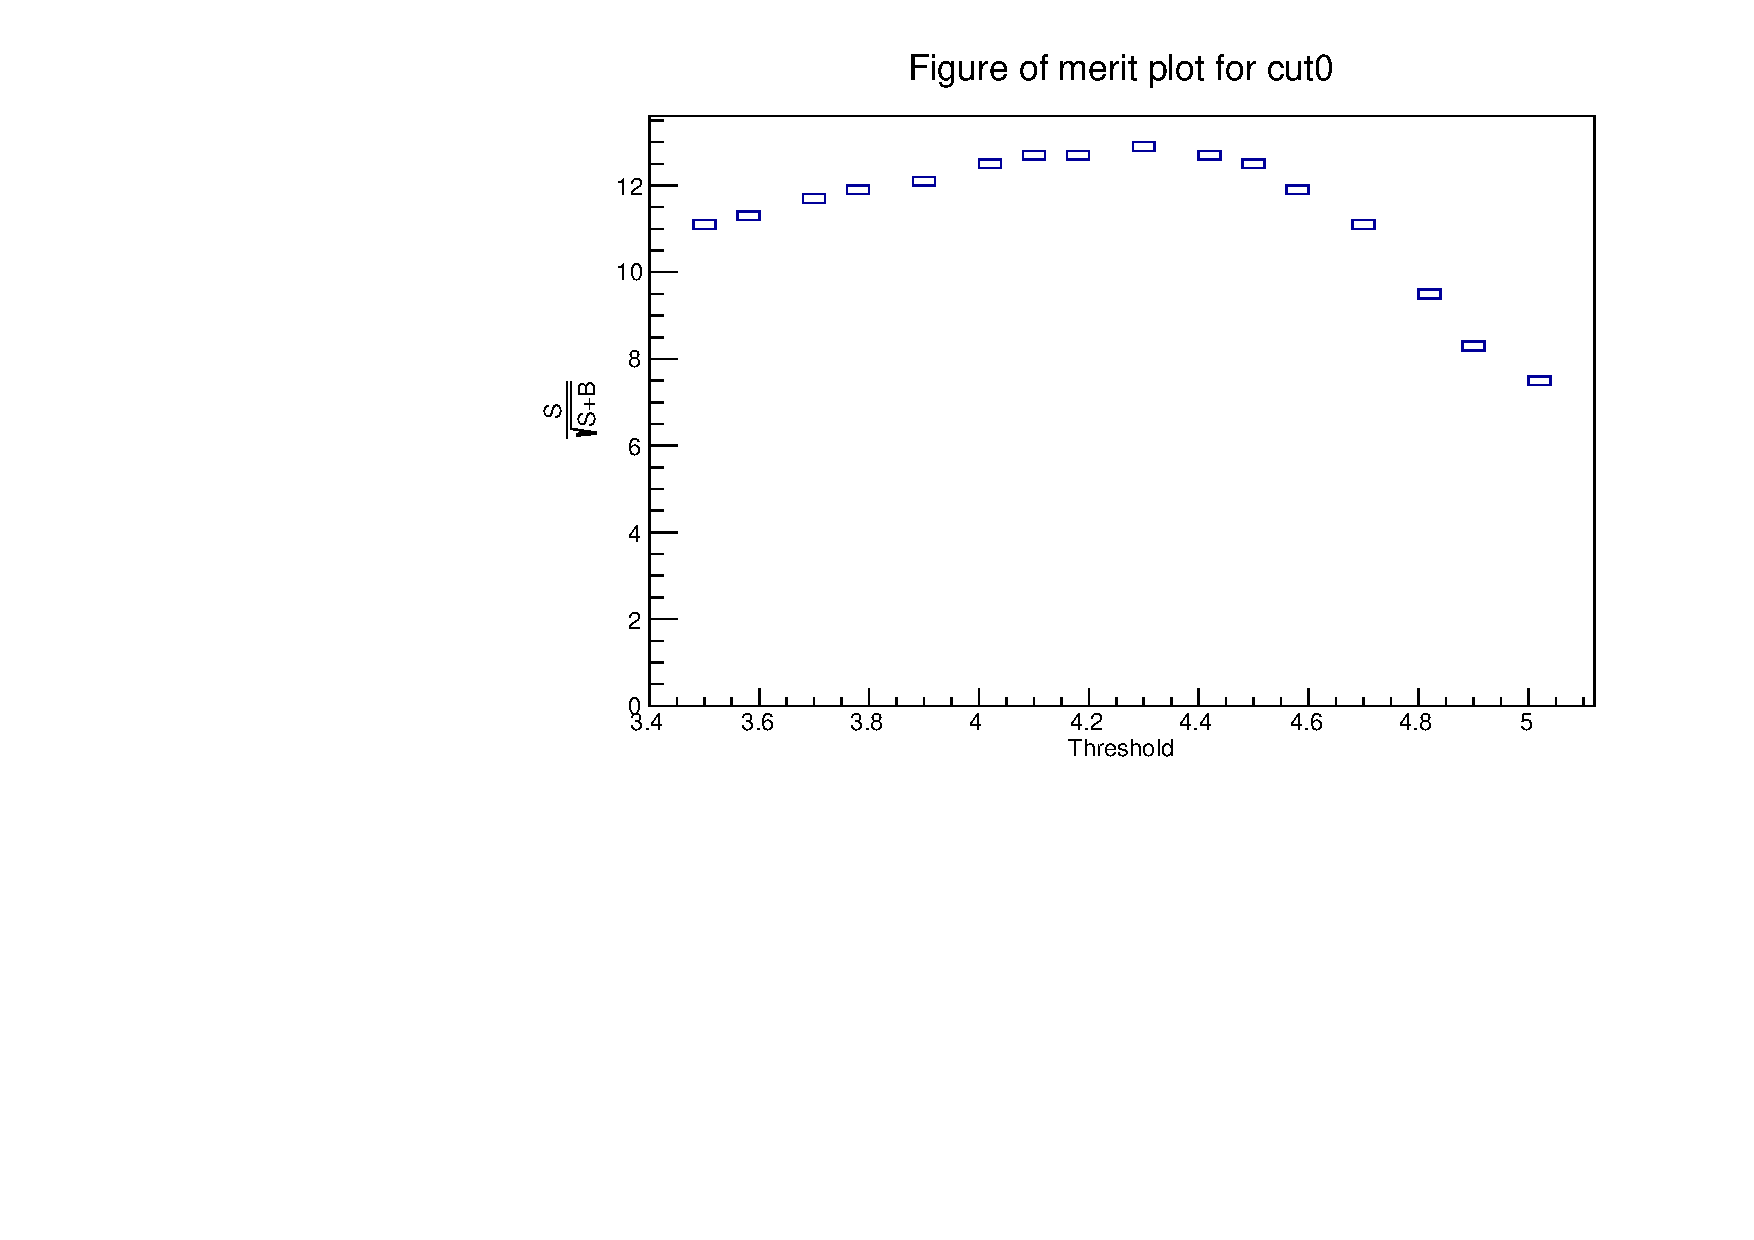
\includegraphics[width=0.7\linewidth]{images/fom-cut0.pdf}
\caption[]%
{{\small Figure-of-merit plot for $p_{\text{signal}}^{\text{CM}}$.}}
\label{fig:fom plot muCM P}
\end{figure}

Initial visual inspection was performed by finding obvious separation between signal and many background variables. This was informed by knowledge of event signatures (Chapter~\ref{chp:event signatures}), as well as some figure-of-merit plots as described above. Figures~\ref{fig:good sep} and~\ref{fig:bad sep} are examples of good and poor selection variables. In Figure~\ref{fig:good sep}, large background peaks occuring at less than $\SI{1}{GeV/c}$ and greater than $\SI{4.3}{Gev}$ lead to great separation from signal, which does not peak anywhere in those regions. Figure~\ref{fig:bad sep} offers less than optimal threshold positions, as there is no apparent way to remove any amount of background without also removing a large amount of signal; note that this variable was not included during event selection. 

\begin{figure}[h]
\centering
\begin{minipage}{.475\textwidth}
  \centering
  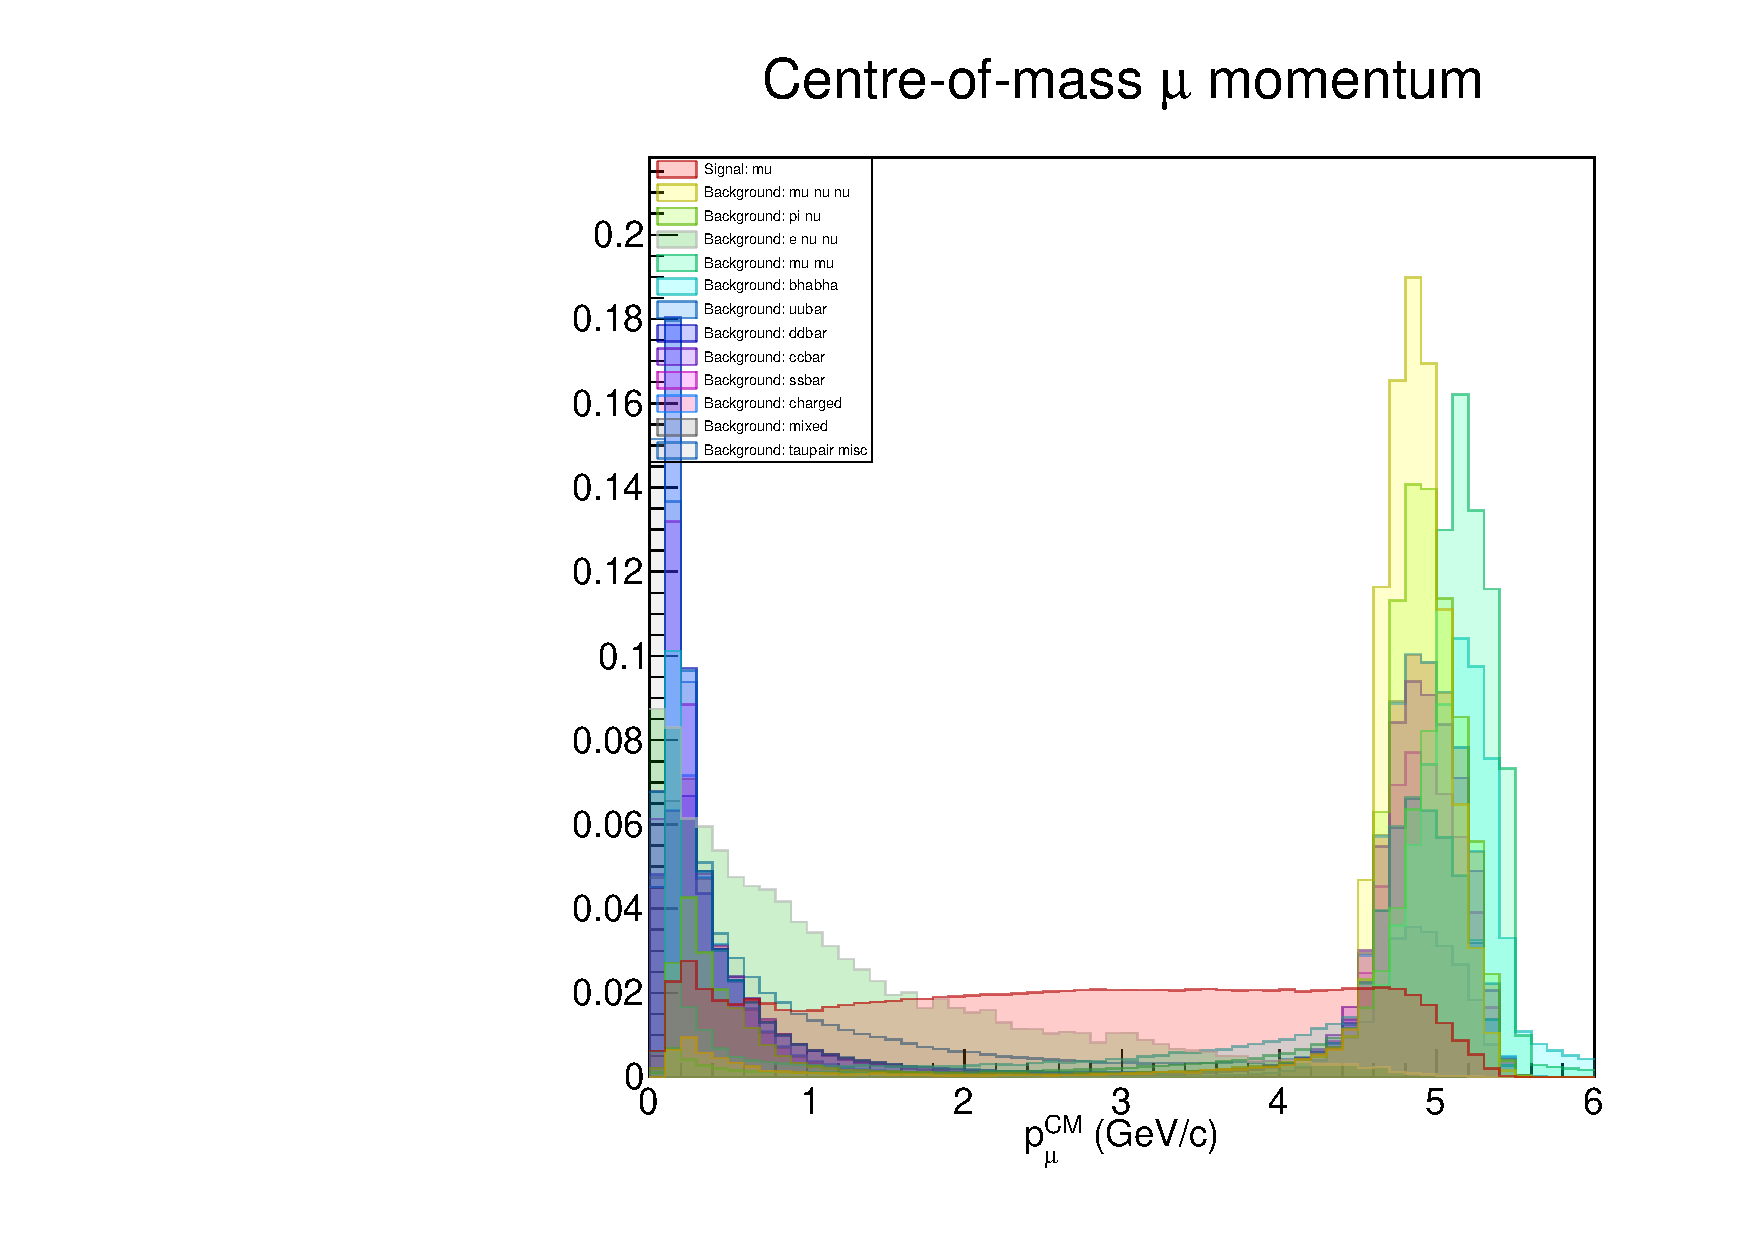
\includegraphics[width=\linewidth]{images/tauMG-muCM_P.pdf}
  \caption[]%
  {\small Center-of-mass frame momentum of signal track.}
  \label{fig:good sep}
\end{minipage}%
\hfill
\begin{minipage}{.475\textwidth}
  \centering
  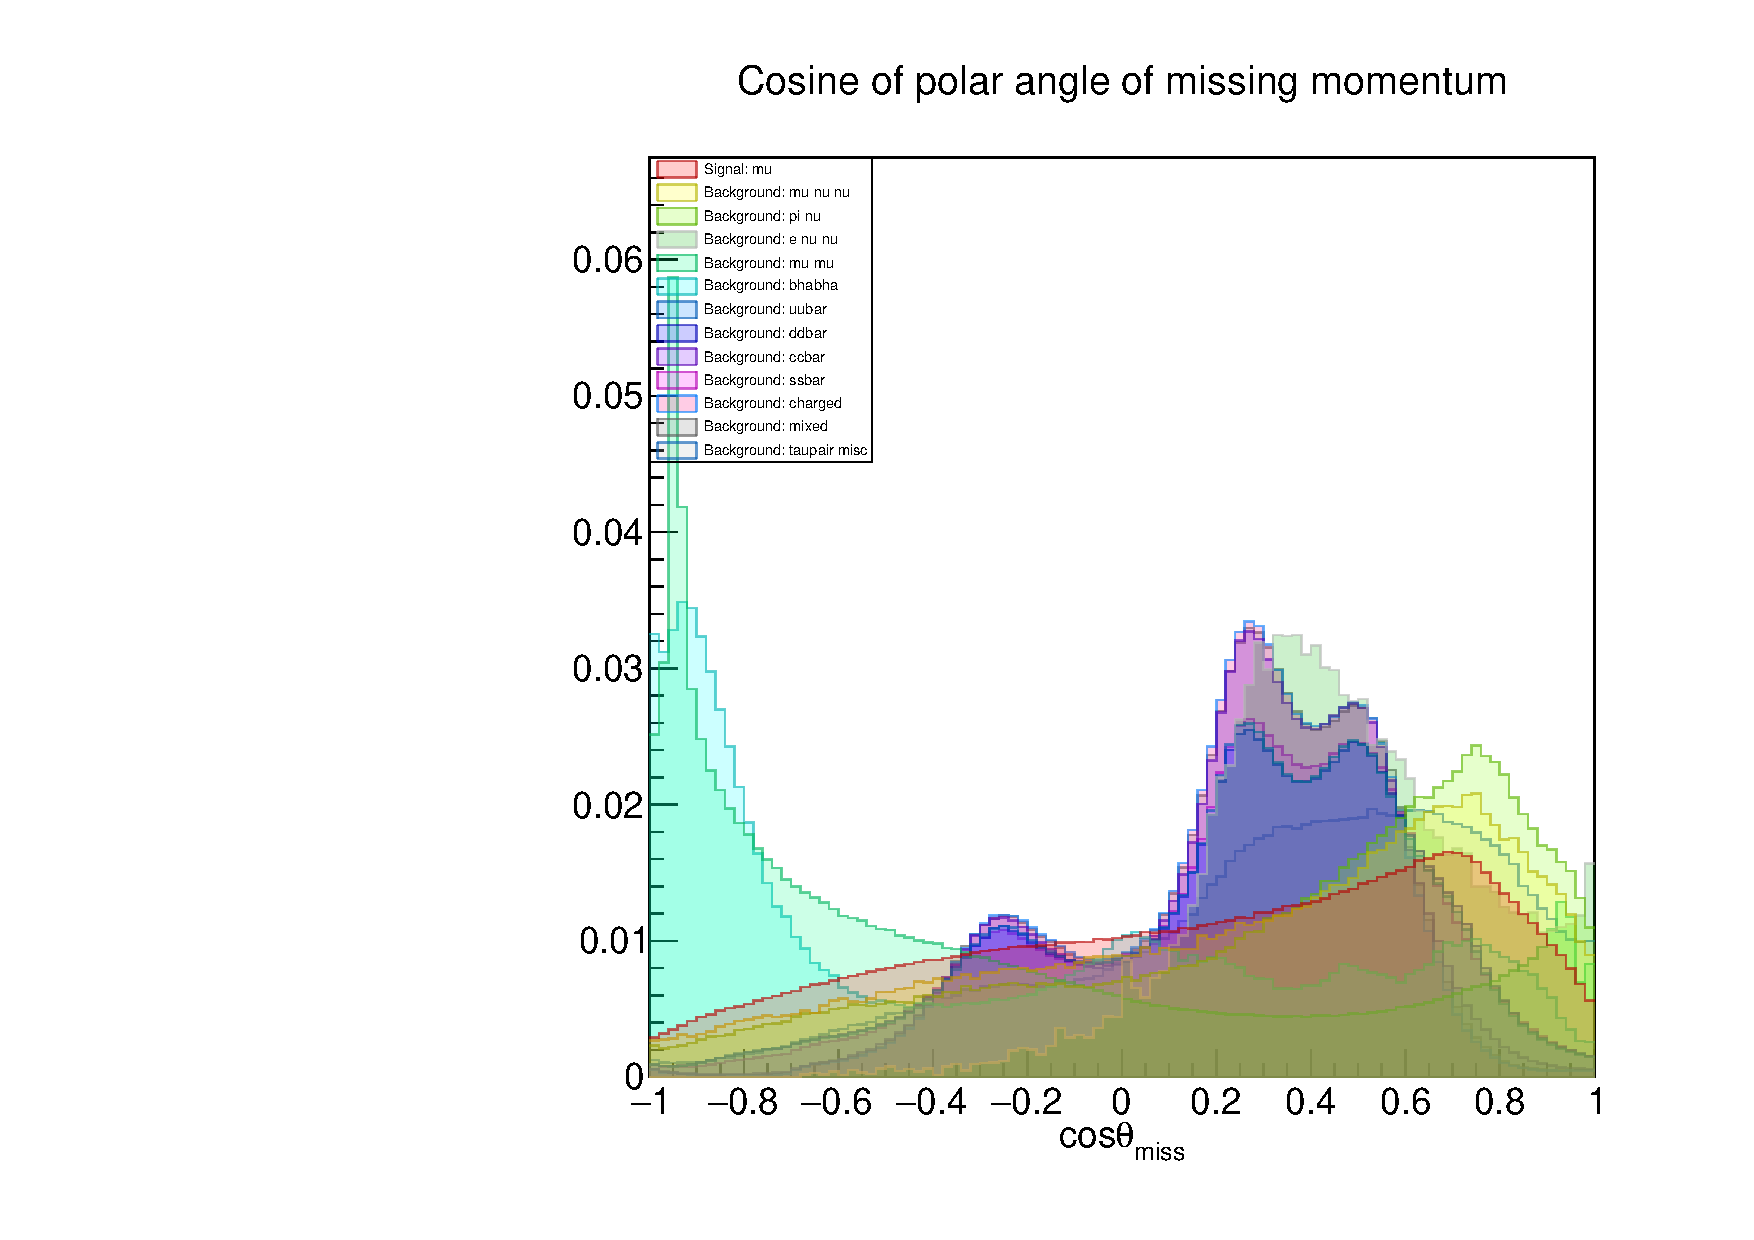
\includegraphics[width=\linewidth]{images/tauMG-missingCosTheta.pdf}
  \caption[]%
  {\small Cosine of polar angle of missing momentum.}
  \label{fig:bad sep}
\end{minipage}
\end{figure}

Following the selection of initial criteria, we performed optimisation by changing certain event requirements then calculating $S/\sqrt{S+B}$. Plots of signal and background were continually produced during this iterative process, with residual backgrounds remaining after selection being analysed. The number of remaining signal events was also considered in optimisation, as some trade-off between maximising $S/\sqrt{S+B}$ and maximising $S$ was sought, due to the low multiplicity of our signal mode.


\section{Selection variables}

Table~\ref{tab:tauMG events after selection} shows the number of signal and background events remaining after selection has been applied. Specific discussion and justification of selection criteria is given below. 

\begin{table}[h]
\centering
\begin{tabular}{lrr}
\textbf{Event process}         & \textbf{events generated} & \textbf{events out} \\ \hline 
\rowcolor[HTML]{EFEFEF} 
$\tau\to\mu\gamma$       & \num{135}        & 6                             \\
$\tau\to\mu\nu\nu$      & \num{631235}             & 163                    \\
$\tau\to\pi\nu$         & \num{822028}                & 40                                     \\
$\tau\to e\nu\nu$       & \num   {70675}              & 0                                  \\
$\tau\to\text{generic}$  & \num{636954}           & 0                                   \\
$e^+ e^- \to \mu^+ \mu^- (\gamma)$       & \num{21938180}        & 15             \\
$e^+ e^- \to e^+ e^- (\gamma)$      & \num{1457005758}      & 0                               \\
$e^+ e^- \to u \bar{u}$       & \num{29767142}           & 9                                 \\
$e^+ e^- \to d \bar{d}$        & \num{7307320}           & 3                                \\
$e^+ e^- \to c \bar{c}$        & \num{23401910}           & 0                            \\
$e^+ e^- \to s \bar{s}$       & \num{6299797}           & 3                                       \\
$e^+ e^- \to B^+ B^-$     & \num{22083348}           & 0                            \\
$e^+ e^- \to B^0 \bar{B}^0$       & \num{23372366}           & 0                           
\end{tabular}
\caption[]%
{{\small Events remaining after selection (muon mode)}}
\label{tab:tauMG events after selection}
\end{table}

\subsection{Energy-momentum}

We require $p^{\text{CM}}_{\mu}$ greater than $\SI{1}{GeV/c}$ and less than $\SI{4.3}{GeV/c}$, to remove low-momentum tracks from continuum events and to remove high-momentum tracks from leptonic processes without high-energy final state photons, that is, generic tau-pair processes, mu-pair processes, and bhabha. Muon transerve momentum $p^{\text{t}}_{\mu}$ is required to be greater than $\SI{0.1}{GeV/c}$; tracks with a lesser transverse momentum could not reach the CDC sub-detector component so we do not select these events. Low-energy tracks from continuum events often do not satisfy this criteria, however most low-energy tracks are excluded through selection on $p^{\text{CM}}_{\mu}$. To suppress $\mu^+\mu^-$ and Bhabha backgrounds we require center-of-mass momentum of the tag track $p^{\text{CM}}_{\text{tag track}}$ less than $\SI{2.5}{GeV}$. Through conservation of momentum we expect the signal and tag tracks of the processes $e^+ e^-\to\ell^+ \ell^- (\gamma)$ we to have momentum peaks around $\SI{5}{GeV}$, which are excluded by this selection. Since most background processes reconstruct the signal photon from low-energy photons, we require the energy of the signal photon $E_{\gamma}$ to be $\SI{0.8}{GeV}$. This selection criteria is effective in removing background events across different processes. Total energy in the center-of-mass frame $E^{\text{CM}}_{\text{total}}$ is required to be less than $\SI{12}{GeV}$ to suppress $\mu^+\mu^-$ events.

\subsection{Angular relations}

As discussed in Chapter~\ref{chp:event signatures}, angular distributions of reconstruction particles depend strongly on the decay process and hence can be used as discriminating variables. For this analysis, $\cos\theta_{\mu}$ is required to be in the range \num{-0.8} to \num{0.9} to suppress continuum, mupair and Bhabha processes. Cosine of the signal photon polar angle $\cos\theta_{\gamma}$ is required to be less than \num{0.85}. We require the polar angle of the reconstructed signal $\tau$ in the center-of-mass frame to be between \num{1} and \num{2.2}. Note that these variables are correlated and overlap in the background which is removed by this selection. Selection is also made on the cosine of the helicity angle $\cos\theta_{\text{H}}$, requiring  $-0.8 < \cos\theta_{\text{H}} < 0.8$. The helicity angle is the opening angle between the signal muon in the signal $\tau$ frame, and the boost direction of the $\tau$ in the center-of-mass frame.

\subsection{Particle likelihoods}

Signal-side tracks are identified as muons by requiring $\mathcal{L}_{\mu} > 0.8$. To reduce the effect of double-counting, mostly for signal events, we require $\mathcal{L}_{K} < 0.08$ and $\mathcal{L}_{e} < 0.005$. We also require $\mathcal{L}_{\pi} > 0.8$. On the tag-side, we require $\mathcal{L}_{\mu} < 0.85$ to identify the tag-track as not a muon. Definitions of particle likelihoods and related plots are discussed at Section~\ref{sec:PID}.

\subsection{Background suppression using event shape}

The thrust axis for a collection of $N$ particles with momenta $\mathbf{p}_{i}$ ($i = 1,\ldots, N$) is defined as the unit vector along with the total projection of these momenta is maximised. The thrust scalar, or thrust, is defined as
\begin{equation}
T = \frac{\sum^N_{i=1}\lvert\mathbf{T}\cdot\mathbf{p}_i\rvert}{\sum^N_{i=i}\lvert\mathbf{p}_i\rvert}.
\end{equation}
Signal thrust and rest-of-event thrust variables are used for selection. The signal thrust axis is constructed from all particles used to reconstruct the signal-side $\tau$; for our signal mode these are the signal muon and signal photon. On average these particles have similar momentum and a small opening between them, so that signal thrust has a clear peak around \num{0.942}. We consider the signal thrust axis for the other dominant leptonic processes. For most events the signal-side is reconstructed from a high-energy charged track and a low-energy photon generated from bremsstrahlung, beam background or similar (radiative mu-pair or Bhabha events can generate higher energy final-state photons). Regardless of opening angle, the difference in momentum between signal track and signal photon leads to signal thrust for this event peaking around \num{1}. A requirement for signal thrust to be in the range \num{0.936} to \num{0.944} to suppress leptonic backgrounds as shown in Figure~\ref{fig:tauMG signal thrust}. 

\begin{figure}[h]
\centering
\begin{minipage}{.475\textwidth}
  \centering
  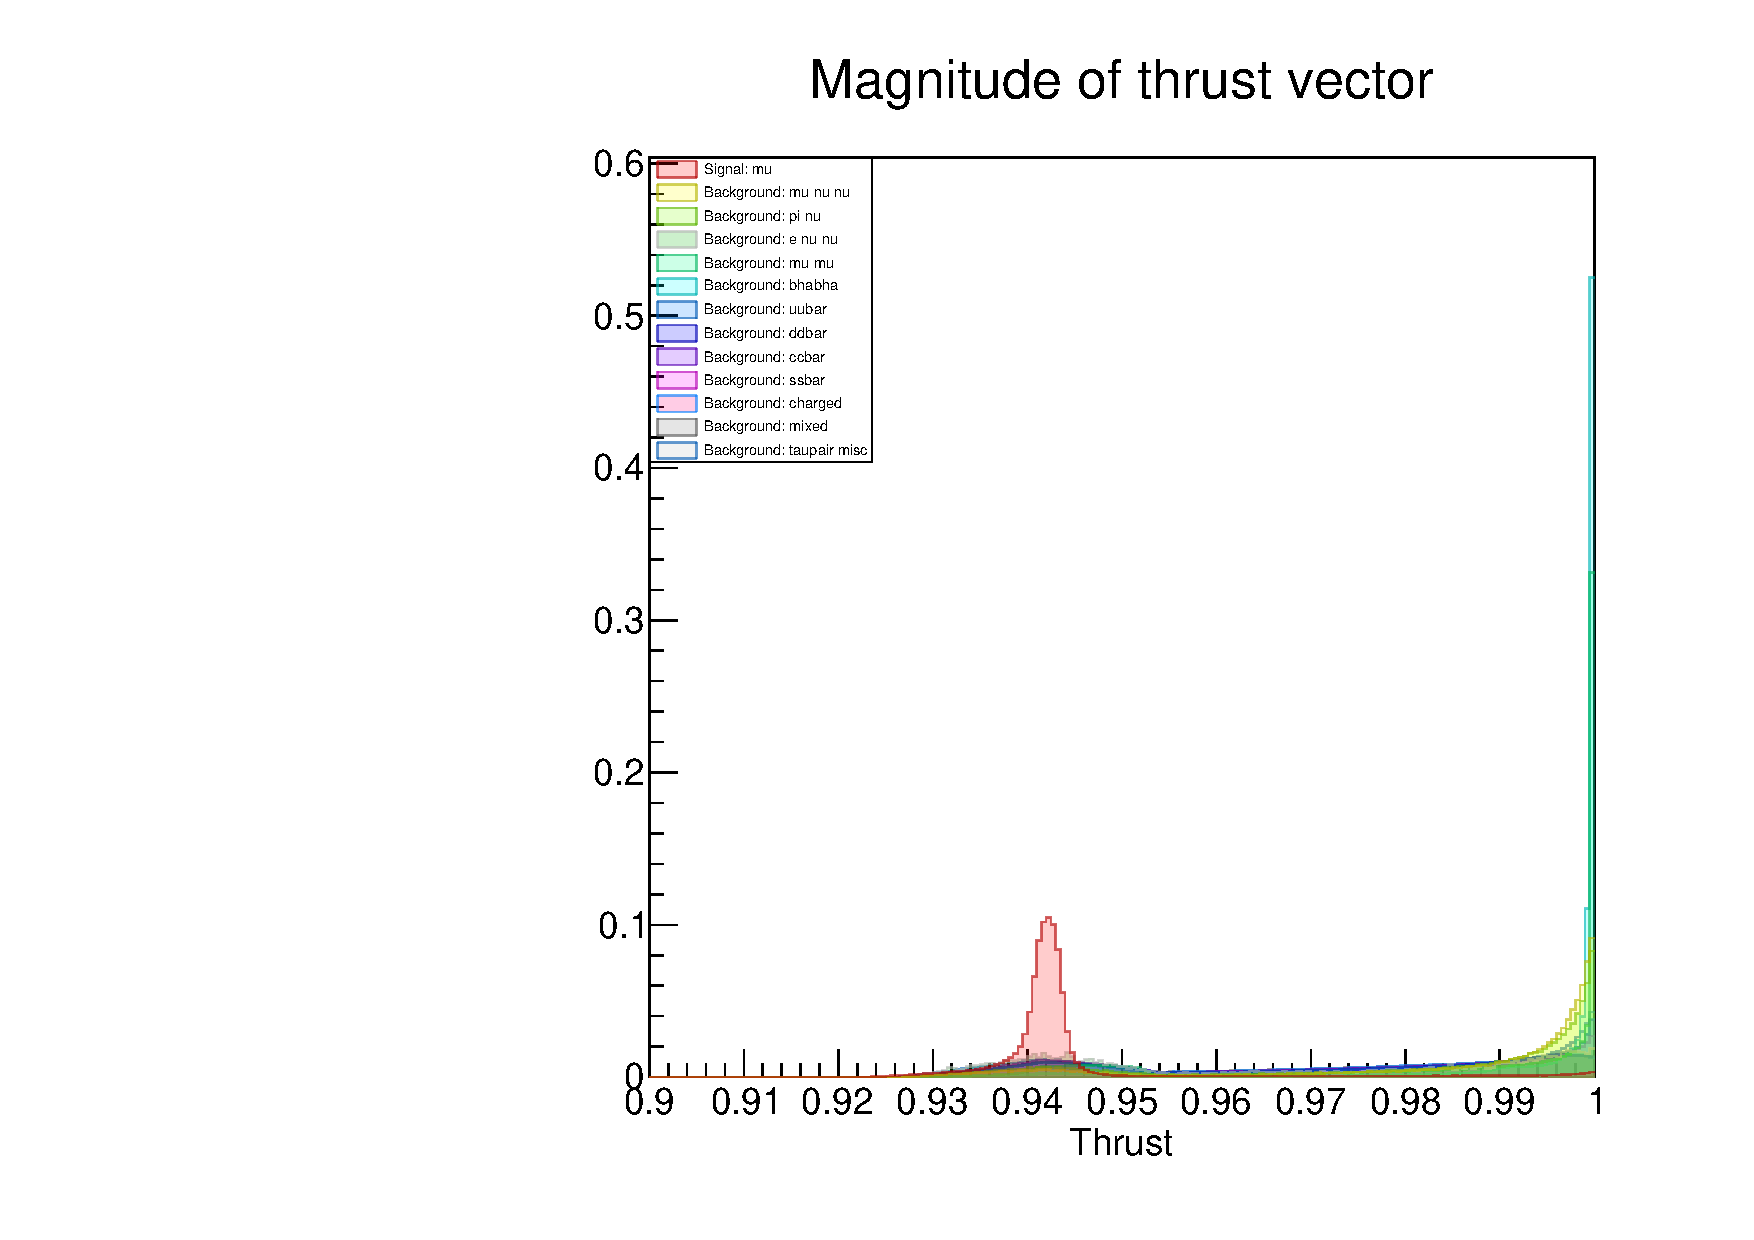
\includegraphics[width=\linewidth]{images/tauMG-thrustSignal.pdf}
  \caption[]%
  {{\small Signal thrust.}}
  \label{fig:tauMG signal thrust}
\end{minipage}%
\hfill
\begin{minipage}{.475\textwidth}
  \centering
  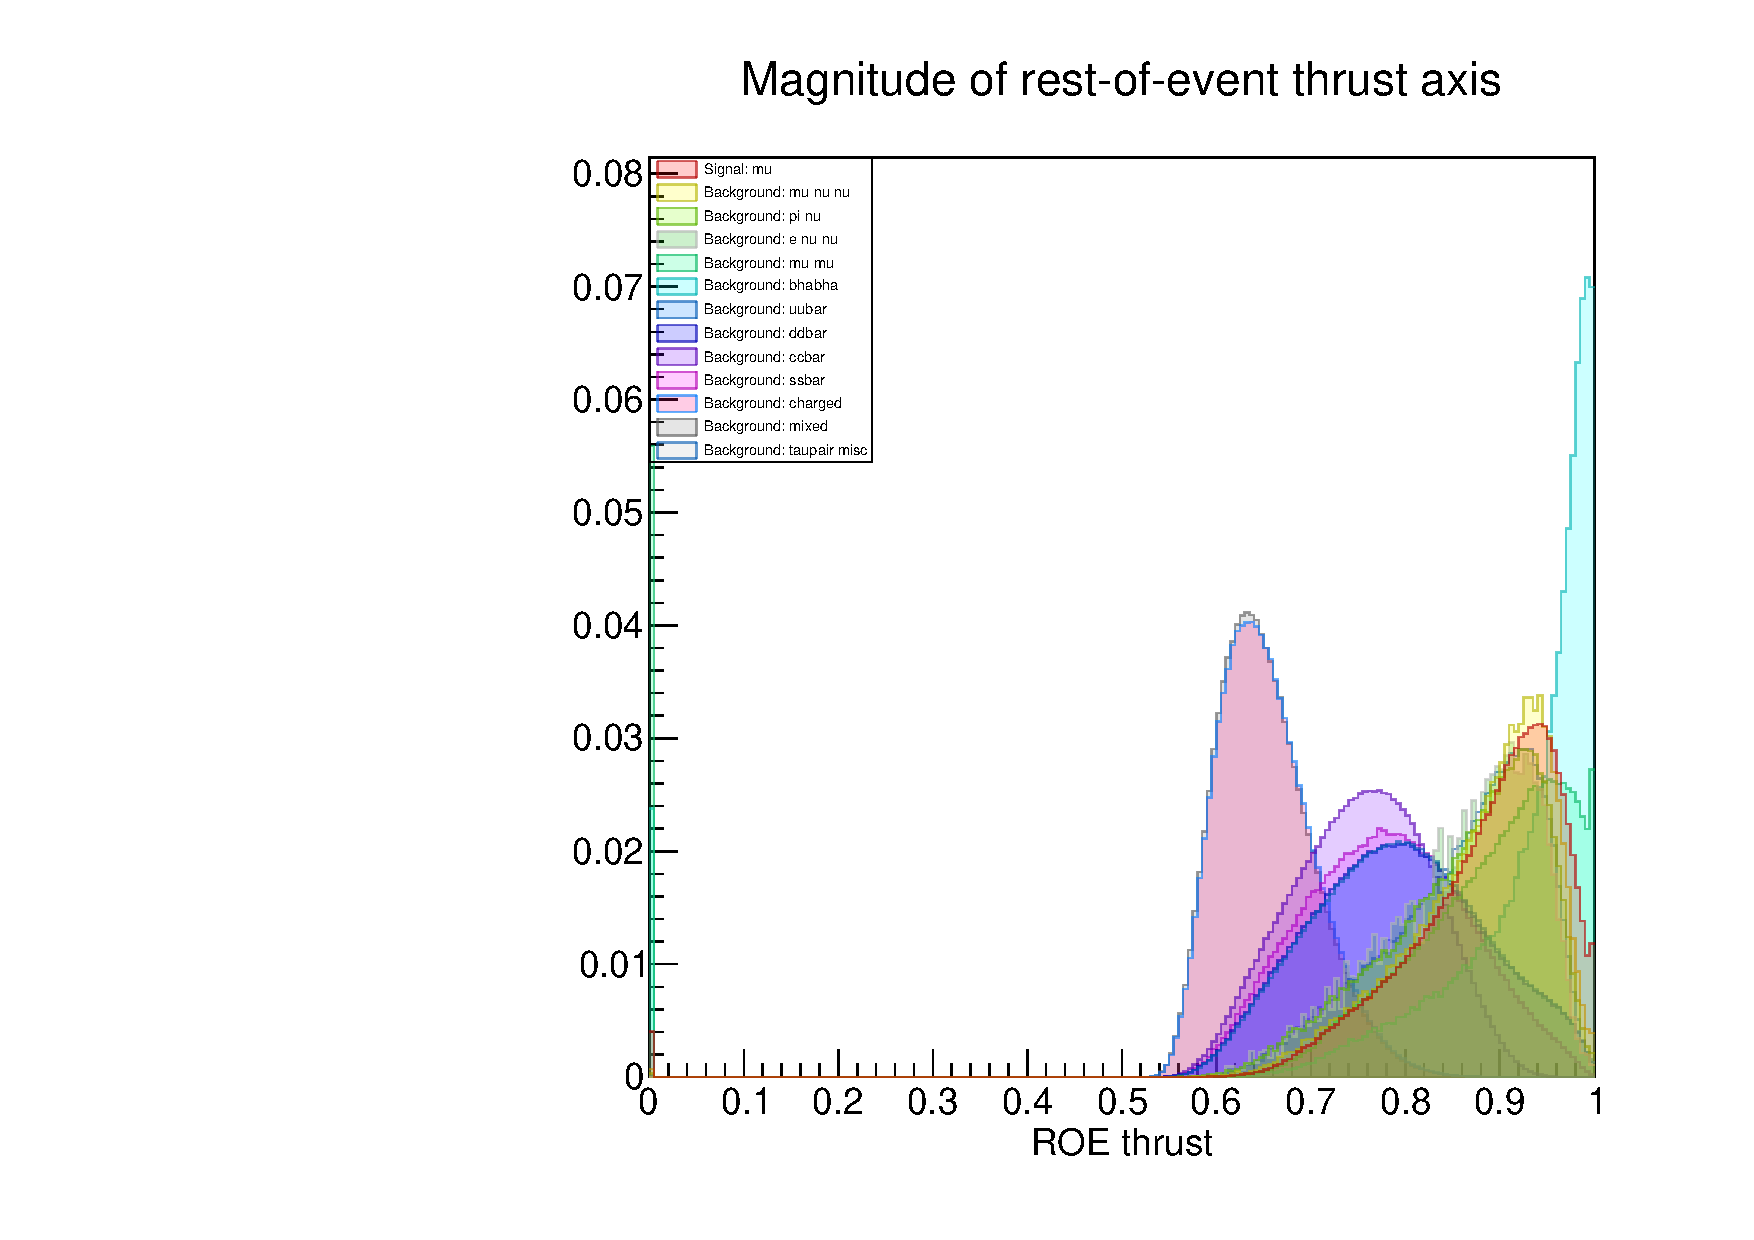
\includegraphics[width=\linewidth]{images/tauMG-thrustRoe.pdf}
  \caption[]%
  {{\small Rest-of-event thrust.}}
  \label{fig:tauMG ROE thrust}
\end{minipage}
\end{figure}


We construct another thrust axis is also built using rest-of-event (ROE) data. ROE comprises all tracks and clusters not associated with the signal-side reconstruction, and so ROE thrust is influenced by tag-side events. Hadronic processes such as $B\bar{B}$ events and continuum have on average a lower rest-of-event thrust than leptonic processes due to the number of tracks and photons produced due to interactions with the detector. The magnitude of this ROE thrust vector is required to be in the range from \num{0.85} and \num{0.98}. As shown in Figure XXXX, events produce very clean Gaussian-like distributions with little trailing tail. As such, while this selection removes a non-negligible amount of signal, it suppresses continuum events very strongly and almost completely excludes $B\bar{B}$ events. Event selection is also performed using the angle between thrust axes. We require the cosine of the angle between the signal thrust vector and rest-of-event thrust vector to be greater than \num{0.7}.


Several continuum suppression variables were chosen by inspection after many more obvious criteria had been applied. These are CLEO cones, Super Fox-Wolfram moments, and the reduced Fox-Wolfram moment (the ratio of the second to the zeroth Fox-Wolfram moments).

Inherent differences in event shape can be used to suppress backgrounds. Some useful disciminant variables are the CLEO cones, named as such due to being introduced in a 1995 paper by the CLEO collaboration\cite{cleo-cones}. To calculate these variables, the space around the signal thrust axis is divided into cones at nine polar angle intervals of $10^{\circ}$ each, with the $i^{th}$ interval covering angles from $(i-1)\times 10^{\circ}$ to $i\times 10^{\circ}$ from the thrust axis (see Figure~\ref{fig:cleo cone image}). Forward and backward intervals are combined. CLEO cone variables cc$i$ are defined as the lab-frame momentum flow of the $i^{th}$ cone; momentum flow in each cone is calculated as the scalar sum of all tracks and clusters in that cone. Requirements on CLEO cones are given in Table~\ref{tab:cleo cone cuts}.


\begin{figure}[h]
\centering
\begin{minipage}{.475\textwidth}
  \centering
	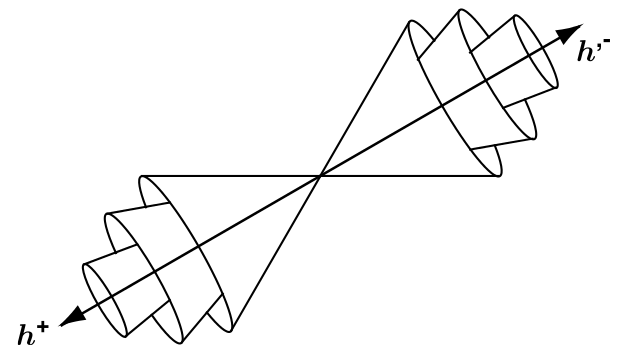
\includegraphics[width=\linewidth]{images/cleo-cone.png}
	\caption[]%
	{{\small Illustration of CLEO cones.}}
	\label{fig:cleo cone image}
\end{minipage}%
\hfill
\begin{minipage}{.475\textwidth}
\centering
\begin{tabular}{lll}
\textbf{CLEO cone} & \multicolumn{1}{c}{\textbf{lower}} & \multicolumn{1}{c}{\textbf{upper}} \\ \hline
cc1 & -- & \num{5} \\
cc2 & \num{2.4} & -- \\
cc3 & -- & -- \\
cc4 & -- & \num{1.7} \\
cc5 & -- & \num{0.9} \\
cc6 & -- & \num{0.7} \\
cc7 & -- & \num{0.5} \\
cc8 & -- & -- \\
cc9 & -- & \num{0.4}
\end{tabular}
\caption[]%
{{\small CLEO cone selection criteria.}}
\label{tab:cleo cone cuts}
\end{minipage}
\end{figure}

\begin{figure}[h]
\centering
\begin{minipage}{.475\textwidth}
  \centering
  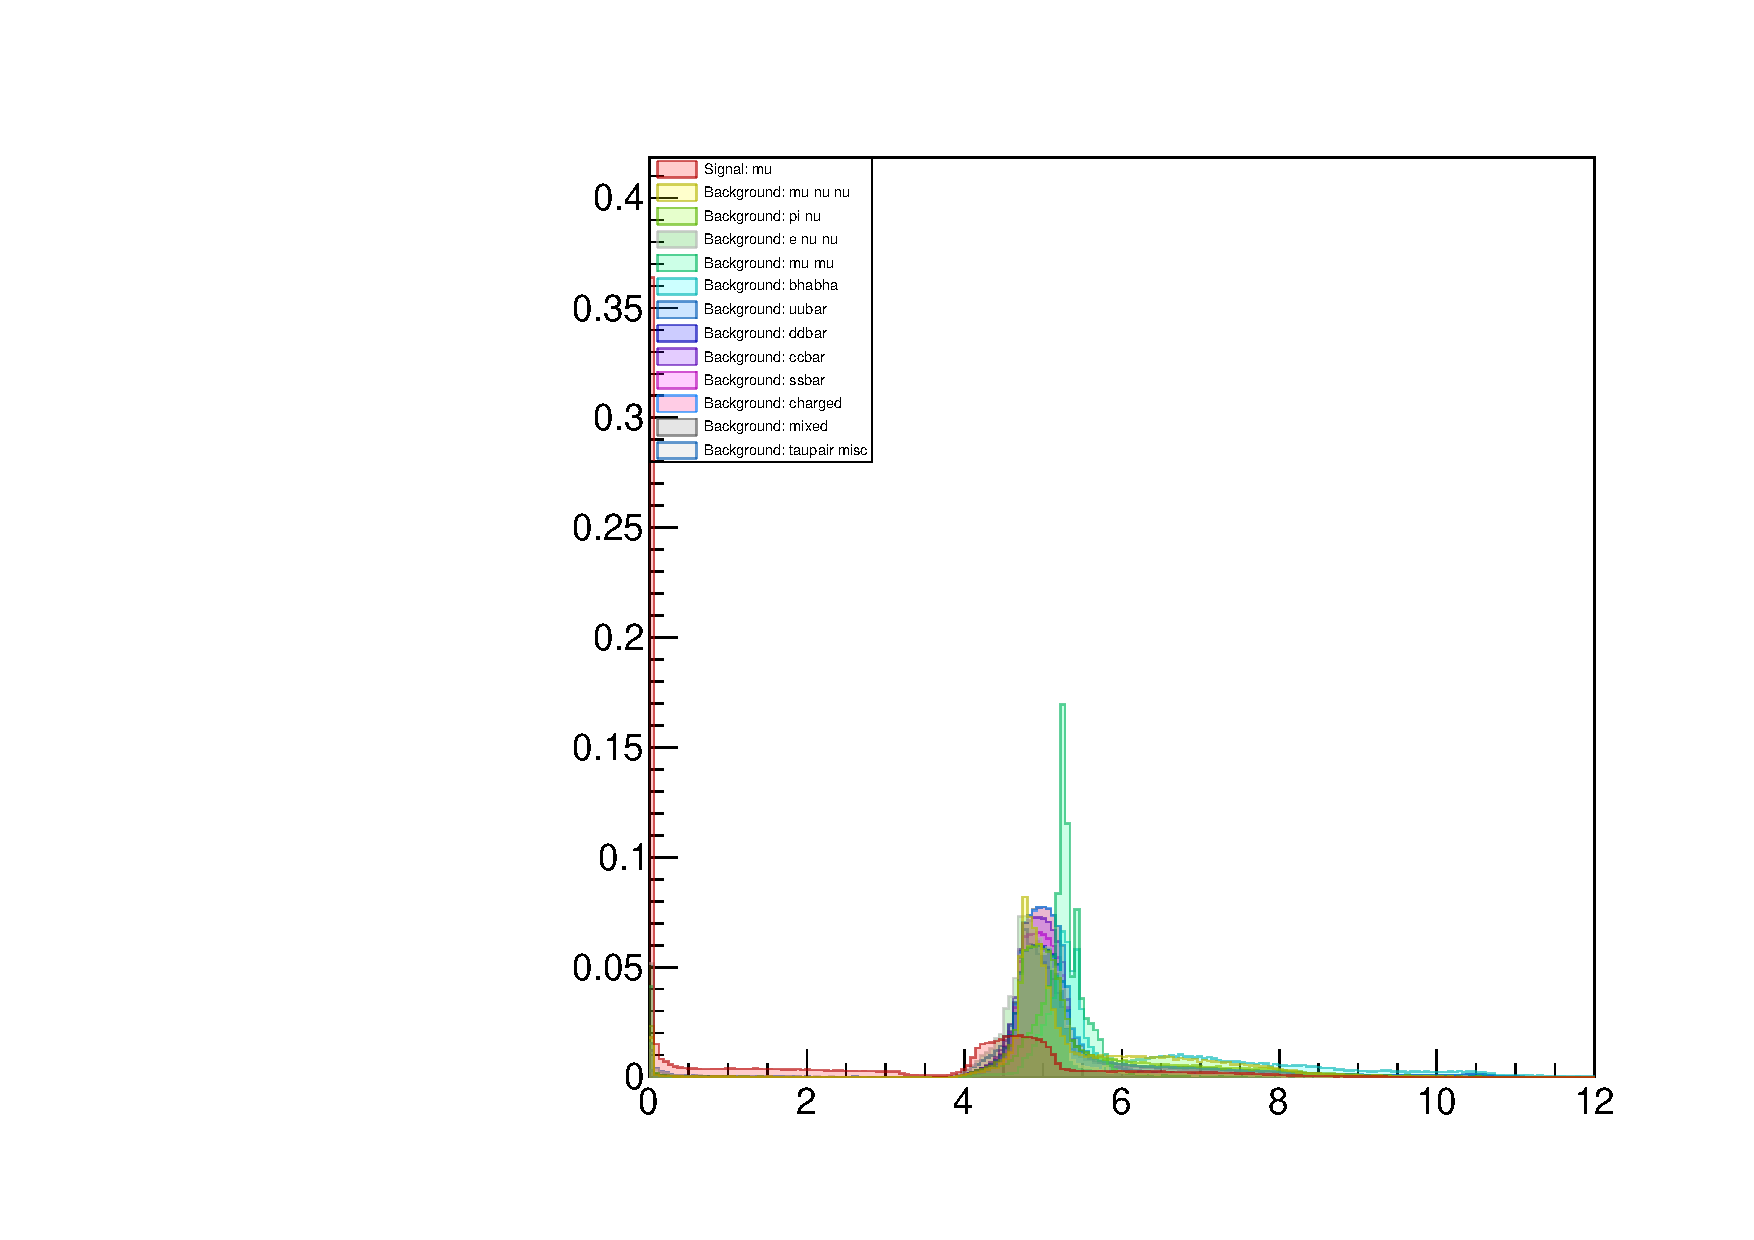
\includegraphics[width=\linewidth]{images/tauMG-cc1.pdf}
  \caption[]%
  {{\small CLEO cone 1.}}
  \label{fig:tauMG cleo cone 1}
\end{minipage}%
\hfill
\begin{minipage}{.475\textwidth}
  \centering
  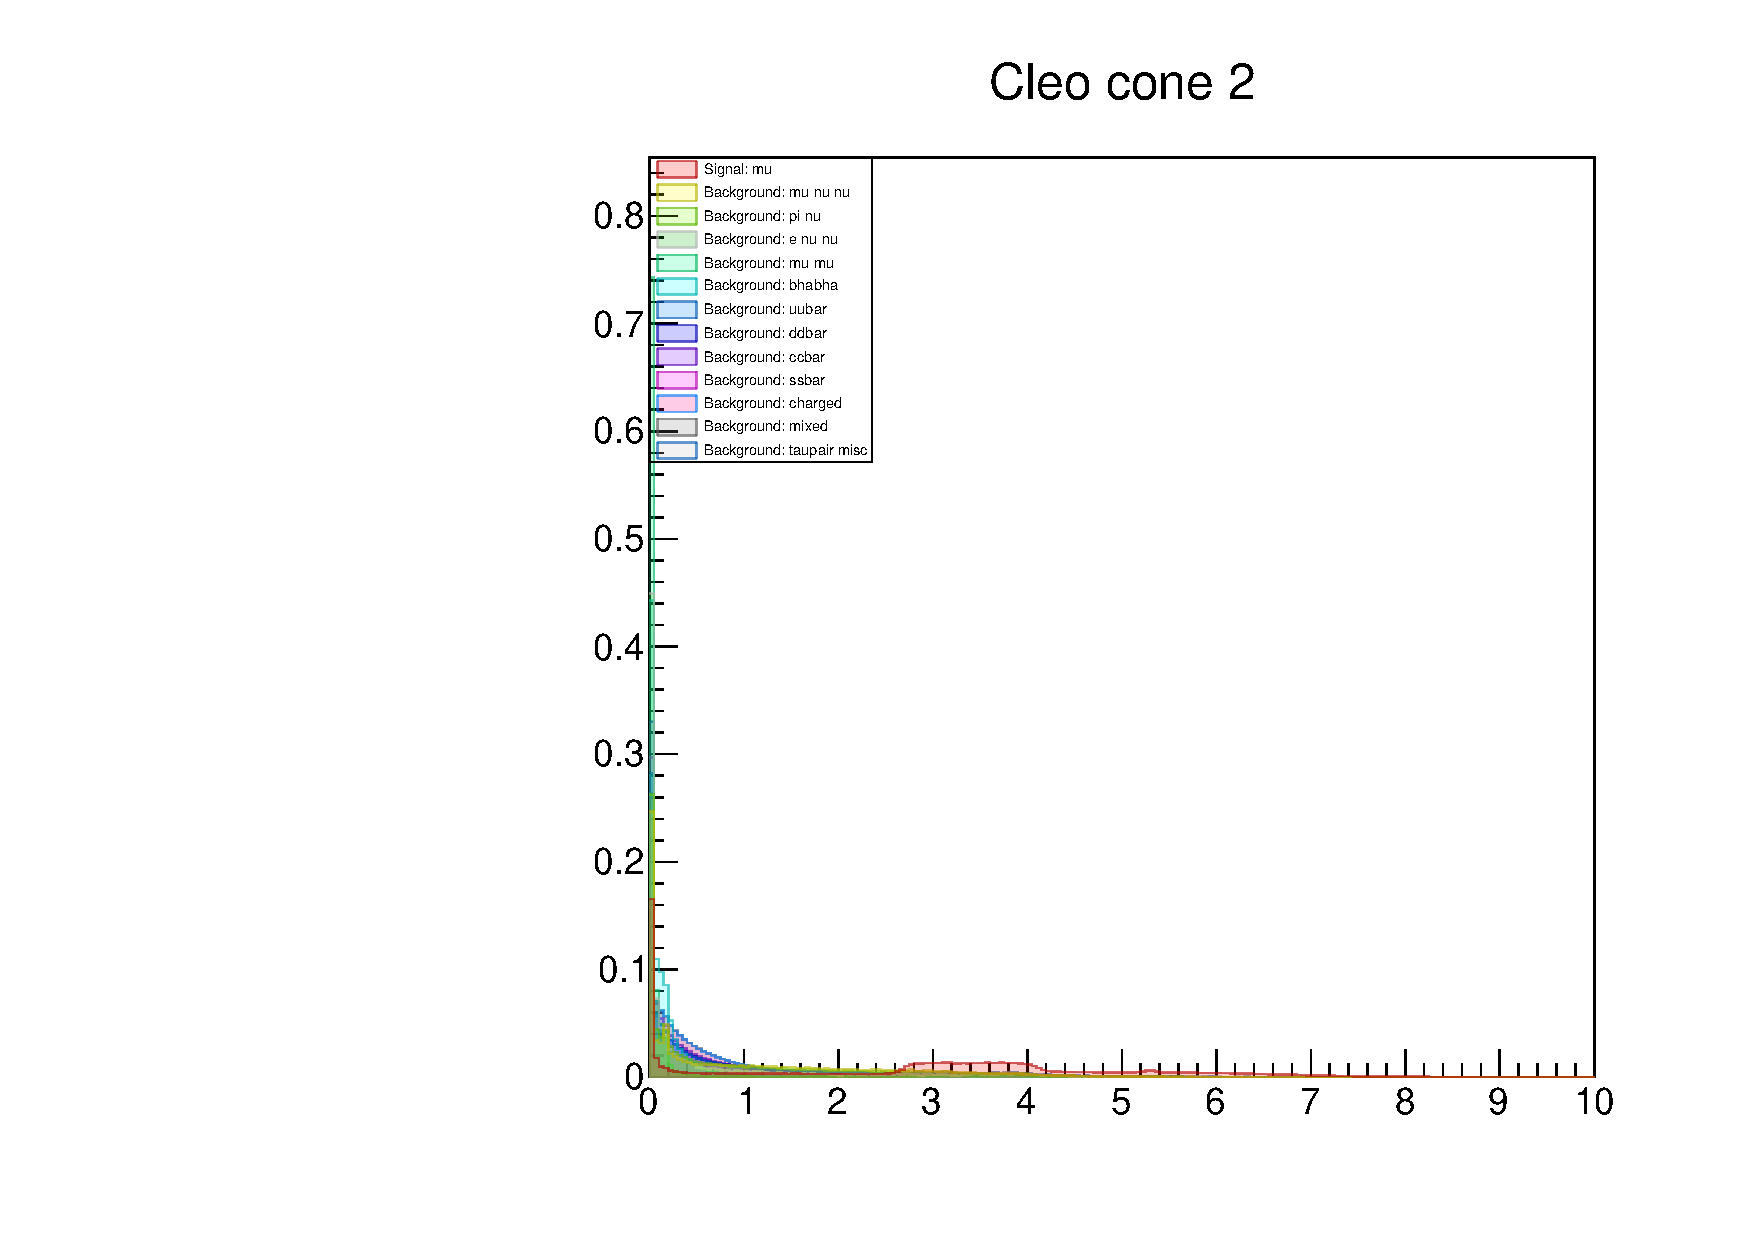
\includegraphics[width=\linewidth]{images/tauMG-cc2.pdf}
  \caption[]%
  {{\small CLEO cone 2.}}
  \label{fig:tauMG cleo cone 2}
\end{minipage}
\end{figure}

Fox-Wolfram moments (FWM) are event shape variables which describe energy flow from high-energy particle collision events, introduced to describe $e^+ e^-$ annihilation event shapes. Variables $h^{so}_i$ ($i=2,4$) and $h^{oo}_j$ are the normalised FWM, defined as
\begin{equation}
h_l^k = \frac{\sum_{m,n}\lvert\vec{p_m}\rvert\lvert\vec{p_n}\rvert P_l(\cos\theta_{mn})}
{\sum_{m,n}\lvert\vec{p_m}\rvert\lvert\vec{p_n}\rvert},
\end{equation}
where $\vec{p_m}$ and $\vec{p_n}$ are the momenta of particles $m$ and $n$ and $P_l(\cos\theta_{mn})$ is the $l$-th other Legendre polynomial of cosine of the angle $\theta_{mn}$ between $\vec{p_m}$ and $\vec{p_n}$. We categorise the type of FWM with $k=so,oo$. For $h^{so}_i$, $m$ is from signal particles and $n$ is from ROE; for $h^{oo}_{j}$ both $m$ and $n$ are from ROE. Fox-Wolfram moments $h^{oo}_j$ are sometimes written as Roo$(i)$; similarly for $h^{so}_{i}$.

\begin{table}[h]
\centering
\begin{tabular}{lll}
\textbf{FWM} & \multicolumn{1}{c}{\textbf{lower}} & \multicolumn{1}{c}{\textbf{upper}} \\ \hline
Hso(0,0) & \num{0.05} & \num{1} \\
Hso(0,1) & \num{-0.05} & \num{0.3} \\
Hso(0,2) & -- & \num{0.48} \\
Hso(0,3) & \num{-0.1} & \num{0.25} \\
Hso(2,0) & \num{-0.1} & \num{1} \\
Roo(1) & \num{-0.018} & \num{0.08} \\
Roo(3) & \num{-0.01} & \num{0.007}
\end{tabular}
\caption{Super Fox-Wolfram moment selection criteria}
\label{my-label}
\end{table}

Two other event shape variable requirement are required on the reduced Fox-Wolfram moment $R_2$ --- the ratio of the second to the zeroth Fox-Wolfram moments --- and the cosine of the angle between the signal thrust axis and the beam axis $\cos\theta_{\text{TBz}}$. We require $R_2 > 0.4$ and $\cos\theta_{\text{TBz}} < 0.8$, with both variables providing good background suppression as seen from Figures~\ref{fig:tauMG R2} and~\ref{fig:tauMG cosTBz}.

\begin{figure}[h]
\centering
\begin{minipage}{.475\textwidth}
  \centering
  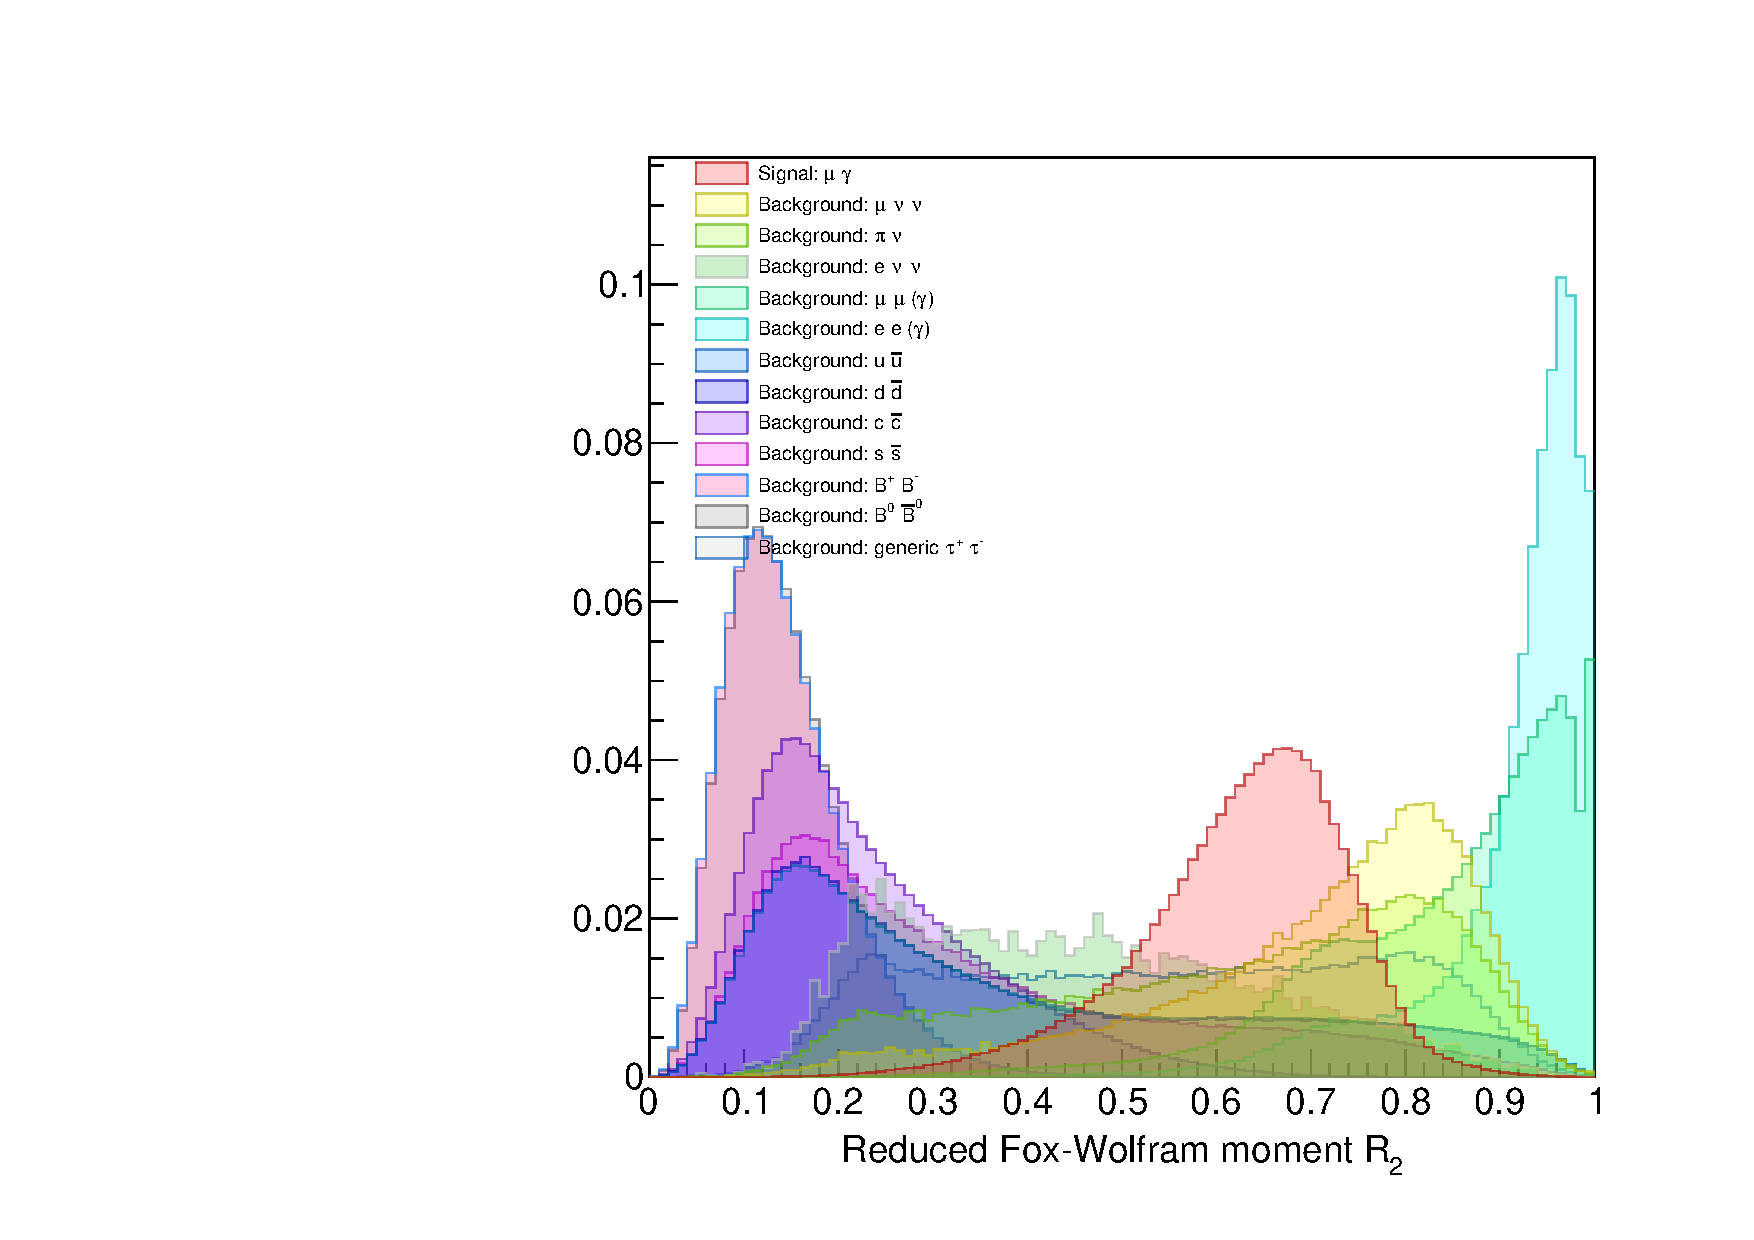
\includegraphics[width=\linewidth]{images/tauMG-R2.pdf}
  \caption[]%
  {{\small Reduced Fox-Wolfram moment $R_2$.}}
  \label{fig:tauMG R2}
\end{minipage}%
\hfill
\begin{minipage}{.475\textwidth}
  \centering
  \includegraphics[width=\linewidth]{images/tauMG-cosTBz.pdf}
  \caption[]%
  {{\small Cosine of the angle between the thrust axis of the signal track and z-axis.}}  \label{fig:tauMG cosTBz}
\end{minipage}
\end{figure}


\subsection{Remaining criteria}

We require the number of reconstructed tracks to be less than 15 to suppress hadronic backgrounds. Selection is also made on the total energy deposited across all ECL clusters by neutral particles, in the range of 2 to $\SI{6}{GeV}$. The ECL energy cluster ratio E9oE25 peaks close to 1 for the signal mode, since the signal photon carries a large fraction of total energy deposited in the ECL. We require E9oE25 greater than \num{0.95} to suppress tau-pair backgrounds.

The emission of a photon after the short $\tau$ lifetime via $\tau\to\mu\gamma$ gives cluster timing peak around zero with a tight width, so we require this variable to be in the range $\SI{-1}{ns}$ to $\SI{1}{ns}$. We apply selection on impact parameters for the signal track $d0$ and $z0$, where $d0$ is the signed distance from the point-of-closest-approach (POCA) to the interaction point, and $z0$ is the $z-$ coordinate of the POCA. We require $-0.05 < d_0 < 0.05$ and $-0.06 < z_0 < 0.06$ for the signal track. These impact parameter variables become more important when analysing actual data rather than MC, due to collisions of detector geometries. Hence while these selection criteria to not discriminate background in a major way in MC, they may become more important when running over Belle II data.

\begin{figure}
\centering
\begin{minipage}{.475\textwidth}
  \centering
  \includegraphics[width=\linewidth]{images/tauMG-neutralEclEnergy.pdf}
  \caption[]%
  {{\small Total energy deposited in ECL clusters by neutral particles.}}    
  \label{fig:tauMG neutralEclEnergy}
\end{minipage}%
        \hfill
\begin{minipage}{.475\textwidth}
  \centering
  \includegraphics[width=\linewidth]{images/tauMG-tracks.pdf}
  \caption[]%
  {{\small Number of reconstructed tracks.}}  
  \label{fig:tauMG tracks}
\end{minipage}
        \vskip\baselineskip
\begin{minipage}{.475\textwidth}
  \centering
  \includegraphics[width=\linewidth]{images/tauMG-sigD0.png}
  \caption[]%
  {{\small Signal track d0.}}    
  \label{fig:tauMG sigD0}
\end{minipage}%
        \hfill
\begin{minipage}{.475\textwidth}
  \centering
  \includegraphics[width=\linewidth]{images/tauMG-sigZ0.png}
  \caption[]%
  {{\small Signal track z0.}}  
  \label{fig:tauMG sigZ0}
\end{minipage}
\end{figure}

\begin{table}[h]
\centering
\begin{tabular}{ll}
\textbf{variable} & \textbf{description} \\ \hline
$p_{\text{signal}}^{\text{CM}}$  & CM momentum of signal track \\
$p_{\text{tag}}^{\text{CM}}$  & CM momentum of tag track  \\
$p_{t~\text{signal}}$ & Transverse momentum of signal track \\
$p_{t~\text{tag}}$ & Transverse momentum of tag track  \\
$\cos\theta_{\text{signal}}$ & Cosine of polar angle of signal track  \\
$\cos\theta_{\text{tag}}$ & Cosine of polar angle of tag track  \\
$E_{\text{total}}^{\text{CM}}$ & Center-of-mass energy of total system    \\
$\text{thrust}_{\text{signal}}$ & Magnitude of signal thrust vector* \\
$\mu\text{-ID}_{\text{signal}}$ & $\mu$ PID of signal track  \\
$\mu\text{-ID}_{\text{tag}}$ & $\mu$ PID of tag track  \\
$E_{\gamma}$ & Energy of signal photon   \\
$\cos\theta_{\gamma}$ & Cosine of polar angle of signal photon   \\
$\cos\theta^{\text{CM}}_{\text{signal}-\gamma}$ & Cosine of center-of-mass frame angle between signal track and signal photon \\
$E_{\text{sum}}^{\text{CM}}$ & Center-of-mass energy of photons and tracks  \\
$\cos\theta^{\text{CM}}_{\text{signal, tag track}}$ & Opening angle between signal and tag track  \\
$\cos\theta_{\text{H}}$ & Cosine of the helicity angle \\
$n_{\text{tracks}}$ & Number of charged tracks  \\
$\text{K-ID}_{\text{signal}}$ & K PID of signal track\\
$\pi\text{-ID}_{\text{signal}}$ & $\pi$ PID of signal track \\
$\text{e-ID}_{\text{signal}}$ & e PID of signal track  \\
\textbf{clusterTiming} & timing of this cluster   \\
\textbf{cosTBz} & Cosine of the angle between the signal thrust axis and z-axis   \\
\textbf{cosTBTO} & Cosine of the angle between the signal thrust axis and ROE thrust axis  \\
$\text{thrust}_{\text{ROE}}$ & Rest-of-event thrust   \\
\textbf{tauCMtheta} & Center-of-mass frame polar angle of reconstructed signal $\tau$ \\
$E_{\text{neutral ECL}}$ & Energy in ECL clusters deposited by neutral particles \\
\textbf{sigD0} & D0 of signal track  \\
\textbf{sigZ0} & Z0 of signal track \\
\textbf{cc1} & Cleo cone 1   \\
\textbf{cc2} & Cleo cone 2 \\
\textbf{cc4} & Cleo cone 4  \\
\textbf{cc5} & Cleo cone 5   \\
\textbf{cc6} & Cleo cone 6  \\
\textbf{cc7} & Cleo cone 7 \\
\textbf{cc9} & Cleo cone 9  \\
\textbf{hso00} & Hso(0,0)  \\
\textbf{hso01} & Hso(0,1)   \\
\textbf{hso02} & Hso(0,2)  \\
\textbf{hso03} & Hso(0,3)  \\
\textbf{hso20} & Hso(2,0)  \\
\textbf{hoo1} & R(1)  \\
\textbf{hoo2} & R(2) \\
\textbf{hoo4} & R(4) \\ \hline
\end{tabular}
\caption{Selection criteria}
\label{tab:selection criteria list}
\end{table}

\begin{comment}
\pagebreak
\begin{sidewaystable}
\tiny
\bigskip
\centering
\begin{tabular}{lcccrrrrrrrrrrrrr}
 & \multicolumn{1}{l}{} & \multicolumn{1}{l}{} & \multicolumn{1}{l}{} & \multicolumn{1}{l}{\textbf{$\tau\to\mu\gamma$}} & \multicolumn{1}{l}{\textbf{$\tau\to\mu\nu\nu$}} & \multicolumn{1}{l}{\textbf{$\tau\to\pi\nu$}} & \multicolumn{1}{l}{\textbf{$\tau\to e\nu\nu$}} & \multicolumn{1}{l}{\textbf{$\tau\to\text{generic}$}} & \multicolumn{1}{l}{\textbf{$e^+ e^- \to \mu^+ \mu^- (\gamma)$}} & \multicolumn{1}{l}{\textbf{$e^+ e^-\to e^+ e^- (\gamma)$}} & \multicolumn{1}{l}{\textbf{$e^+ e^-\to u\bar{u}$}} & \multicolumn{1}{l}{\textbf{$e^+ e^-\to d\bar{d}$}} & \multicolumn{1}{l}{\textbf{$e^+ e^-\to c\bar{c}$}} & \multicolumn{1}{l}{\textbf{$e^+ e^-\to s\bar{s}$}} & \multicolumn{1}{l}{\textbf{$e^+ e^-\to B^+ B^-$}} & \multicolumn{1}{l}{\textbf{$e^+ e^-\to B^0 \bar{B}^0$}} \\
\multicolumn{4}{r}{\textbf{events in}} & \cellcolor[HTML]{EFEFEF}135 & \num{631235} & \num{822028} & \num{70675} & \num{636954} & \num{21938180} & \num{1457005758} & \num{29767142} & \num{7307320} & \num{23401910} & \num{6299797} & \num{22083348} & \num{23372366} \\
 & \multicolumn{1}{l}{\textbf{lower}} & \multicolumn{1}{l}{\textbf{upper}} & \multicolumn{1}{l}{\textbf{\#}} & \cellcolor[HTML]{EFEFEF} &  &  &  &  &  &  &  &  &  &  &  &  \\ \hline
$p_{\text{signal}}^{\text{CM}}$ & \num{1} & \num{4.3} & 0 & \cellcolor[HTML]{EFEFEF}\num{91} & \num{21766} & \num{32974} & \num{7324} & \num{84184} & \num{1429469} & \num{25239923} & \num{1197596} & \num{299166} & \num{1004741} & \num{228377} & \num{378083} & \num{395804} \\
$p_{\text{tag}}^{\text{CM}}$ & \num{} & \num{2.5} & 1 & \cellcolor[HTML]{EFEFEF}\num{85} & \num{21089} & \num{32169} & \num{7139} & \num{81811} & \num{490202} & \num{8291747} & \num{1179381} & \num{294818} & \num{992633} & \num{225315} & \num{373158} & \num{391169} \\
$p_{t~\text{signal}}$ & \num{0.1} & \num{} & 2 & \cellcolor[HTML]{EFEFEF}\num{85} & \num{21089} & \num{32155} & \num{7133} & \num{81811} & \num{490202} & \num{8291747} & \num{1178793} & \num{294748} & \num{992215} & \num{225270} & \num{373015} & \num{390932} \\
$p_{t~\text{tag}}$ & \num{} & \num{} & 3 & \cellcolor[HTML]{EFEFEF}\num{85} & \num{21089} & \num{32155} & \num{7133} & \num{81811} & \num{490202} & \num{8291747} & \num{1178793} & \num{294748} & \num{992215} & \num{225270} & \num{373015} & \num{390932} \\
$\cos\theta_{\text{signal}}$ & \num{-0.8} & \num{0.9} & 4 & \cellcolor[HTML]{EFEFEF}\num{78} & \num{16425} & \num{20003} & \num{4215} & \num{25820} & \num{434015} & \num{1151631} & \num{637526} & \num{160350} & \num{560777} & \num{125241} & \num{232106} & \num{241352} \\
$\cos\theta_{\text{tag}}$ & \num{} & \num{} & 5 & \cellcolor[HTML]{EFEFEF}\num{78} & \num{16425} & \num{20003} & \num{4215} & \num{25820} & \num{434015} & \num{1151631} & \num{637526} & \num{160350} & \num{560777} & \num{125241} & \num{232106} & \num{241352} \\
$E_{\text{total}}^{\text{CM}}$ & \num{} & \num{12} & 6 & \cellcolor[HTML]{EFEFEF}\num{77} & \num{16113} & \num{19718} & \num{4159} & \num{25160} & \num{433111} & \num{1151631} & \num{618179} & \num{155496} & \num{544948} & \num{121108} & \num{226042} & \num{234168} \\
$\lvert\text{thrust}_{\text{signal}}\rvert$ & \num{0.936} & \num{0.944} & 7 & \cellcolor[HTML]{EFEFEF}\num{70} & \num{8224} & \num{9803} & \num{1845} & \num{11175} & \num{167642} & \num{403071} & \num{298024} & \num{74428} & \num{264600} & \num{59129} & \num{109294} & \num{115361} \\
$\mu\text{-ID}_{\text{signal}}$ & \num{0.8} & \num{} & 8 & \cellcolor[HTML]{EFEFEF}\num{67} & \num{6168} & \num{1884} & \num{456} & \num{1869} & \num{162010} & \num{0} & \num{44512} & \num{11100} & \num{35760} & \num{8879} & \num{13695} & \num{14928} \\
$\mu\text{-ID}_{\text{tag}}$ & \num{} & \num{0.85} & 10 & \cellcolor[HTML]{EFEFEF}\num{60} & \num{5428} & \num{1669} & \num{353} & \num{1636} & \num{138602} & \num{0} & \num{38610} & \num{9558} & \num{30404} & \num{7711} & \num{11801} & \num{12914} \\
$E_{\gamma}$ & \num{0.8} & \num{} & 11 & \cellcolor[HTML]{EFEFEF}\num{60} & \num{4616} & \num{1466} & \num{308} & \num{1371} & \num{133202} & \num{0} & \num{30448} & \num{7291} & \num{22971} & \num{5602} & \num{7424} & \num{7831} \\
$\cos\theta_{\gamma}$ & \num{-0.8} & \num{0.85} & 12 & \cellcolor[HTML]{EFEFEF}\num{53} & \num{2485} & \num{899} & \num{300} & \num{1170} & \num{93570} & \num{0} & \num{24532} & \num{6008} & \num{18688} & \num{4530} & \num{5889} & \num{6391} \\
$\cos\theta^{\text{CM}}_{\text{signal}-\gamma}$ & \num{} & \num{} & 13 & \cellcolor[HTML]{EFEFEF}\num{53} & \num{2485} & \num{899} & \num{300} & \num{1170} & \num{93570} & \num{0} & \num{24532} & \num{6008} & \num{18688} & \num{4530} & \num{5889} & \num{6391} \\
$E_{\text{sum}}^{\text{CM}}$ & \num{} & \num{} & 14 & \cellcolor[HTML]{EFEFEF}\num{53} & \num{2485} & \num{899} & \num{300} & \num{1170} & \num{93570} & \num{0} & \num{24532} & \num{6008} & \num{18688} & \num{4530} & \num{5889} & \num{6391} \\
$\cos\theta^{\text{CM}}_{\text{signal, tag track}}$ & \num{} & \num{} & 15 & \cellcolor[HTML]{EFEFEF}\num{53} & \num{2485} & \num{899} & \num{300} & \num{1170} & \num{93570} & \num{0} & \num{24532} & \num{6008} & \num{18688} & \num{4530} & \num{5889} & \num{6391} \\
$\cos\theta_{\text{H}}$ & \num{-0.8} & \num{0.8} & 16 & \cellcolor[HTML]{EFEFEF}\num{53} & \num{2485} & \num{899} & \num{300} & \num{1170} & \num{93570} & \num{0} & \num{24532} & \num{6008} & \num{18688} & \num{4530} & \num{5889} & \num{6391} \\
$n_{\text{tracks}}$ & \num{} & \num{15} & 21 & \cellcolor[HTML]{EFEFEF}\num{53} & \num{2460} & \num{858} & \num{266} & \num{1131} & \num{93570} & \num{0} & \num{20196} & \num{4817} & \num{13328} & \num{3835} & \num{2623} & \num{2641} \\
Cluster timing & \num{-1} & \num{1} & 22 & \cellcolor[HTML]{EFEFEF}\num{44} & \num{1861} & \num{618} & \num{178} & \num{829} & \num{9595} & \num{0} & \num{13037} & \num{3083} & \num{8580} & \num{2209} & \num{1403} & \num{1474} \\
$\text{K-ID}_{\text{signal}}$ & \num{} & \num{0.08} & 23 & \cellcolor[HTML]{EFEFEF}\num{44} & \num{1861} & \num{618} & \num{178} & \num{829} & \num{9595} & \num{0} & \num{13037} & \num{3083} & \num{8580} & \num{2209} & \num{1403} & \num{1474} \\
$\pi\text{-ID}_{\text{signal}}$ & \num{0.8} & \num{} & 24 & \cellcolor[HTML]{EFEFEF}\num{39} & \num{1683} & \num{570} & \num{140} & \num{299} & \num{9008} & \num{0} & \num{9353} & \num{2140} & \num{6501} & \num{1345} & \num{1058} & \num{1137} \\
$\text{e-ID}_{\text{signal}}$ & \num{} & \num{0.005} & 25 & \cellcolor[HTML]{EFEFEF}\num{39} & \num{1600} & \num{530} & \num{10} & \num{95} & \num{9008} & \num{0} & \num{5410} & \num{1246} & \num{3679} & \num{720} & \num{478} & \num{658} \\
$\lvert\text{thrust}_{\text{ROE}}\rvert$ & \num{0.85} & \num{0.98} & 31 & \cellcolor[HTML]{EFEFEF}\num{26} & \num{1054} & \num{350} & \num{10} & \num{89} & \num{3306} & \num{0} & \num{1633} & \num{358} & \num{640} & \num{161} & \num{0} & \num{5} \\
cc1 & \num{} & \num{5} & 33 & \cellcolor[HTML]{EFEFEF}\num{25} & \num{1010} & \num{339} & \num{10} & \num{80} & \num{3276} & \num{0} & \num{1406} & \num{324} & \num{630} & \num{161} & \num{0} & \num{5} \\
hso00 & \num{0.05} & \num{1} & 34 & \cellcolor[HTML]{EFEFEF}\num{19} & \num{793} & \num{229} & \num{10} & \num{60} & \num{178} & \num{0} & \num{529} & \num{173} & \num{145} & \num{25} & \num{0} & \num{0} \\
$E_{\text{ECL, neutrals}}$ & \num{2} & \num{6} & 35 & \cellcolor[HTML]{EFEFEF}\num{15} & \num{630} & \num{163} & \num{0} & \num{44} & \num{100} & \num{0} & \num{218} & \num{73} & \num{78} & \num{16} & \num{0} & \num{0} \\
sigD0 & \num{-0.05} & \num{0.05} & 36 & \cellcolor[HTML]{EFEFEF}\num{15} & \num{581} & \num{113} & \num{0} & \num{1} & \num{100} & \num{0} & \num{171} & \num{58} & \num{43} & \num{3} & \num{0} & \num{0} \\
sigZ0 & \num{-0.06} & \num{0.06} & 37 & \cellcolor[HTML]{EFEFEF}\num{14} & \num{529} & \num{104} & \num{0} & \num{0} & \num{100} & \num{0} & \num{150} & \num{57} & \num{43} & \num{3} & \num{0} & \num{0} \\
E9E25 & \num{0.95} & \num{} & 38 & \cellcolor[HTML]{EFEFEF}\num{14} & \num{526} & \num{101} & \num{0} & \num{0} & \num{100} & \num{0} & \num{114} & \num{54} & \num{34} & \num{3} & \num{0} & \num{0} \\
$R_2$ & \num{0.4} & \num{} & 39 & \cellcolor[HTML]{EFEFEF}\num{13} & \num{520} & \num{90} & \num{0} & \num{0} & \num{100} & \num{0} & \num{114} & \num{54} & \num{25} & \num{3} & \num{0} & \num{0} \\
hoo0 & \num{} & \num{0.15} & 40 & \cellcolor[HTML]{EFEFEF}\num{13} & \num{510} & \num{90} & \num{0} & \num{0} & \num{85} & \num{0} & \num{110} & \num{54} & \num{16} & \num{3} & \num{0} & \num{0} \\
hso10 & \num{} & \num{0.35} & 41 & \cellcolor[HTML]{EFEFEF}\num{12} & \num{443} & \num{85} & \num{0} & \num{0} & \num{54} & \num{0} & \num{66} & \num{16} & \num{8} & \num{3} & \num{0} & \num{0} \\
$\theta^{\text{CM}}_{\tau}$ & \num{1} & \num{2.2} & 44 & \cellcolor[HTML]{EFEFEF}\num{9} & \num{311} & \num{63} & \num{0} & \num{0} & \num{31} & \num{0} & \num{27} & \num{3} & \num{8} & \num{3} & \num{0} & \num{0} \\
cosTBTO & \num{0.7} & \num{} & 45 & \cellcolor[HTML]{EFEFEF}\num{8} & \num{268} & \num{63} & \num{0} & \num{0} & \num{31} & \num{0} & \num{27} & \num{3} & \num{8} & \num{3} & \num{0} & \num{0} \\
cc2 & \num{2.4} & \num{} & 46 & \cellcolor[HTML]{EFEFEF}\num{8} & \num{241} & \num{48} & \num{0} & \num{0} & \num{15} & \num{0} & \num{23} & \num{3} & \num{5} & \num{3} & \num{0} & \num{0} \\
cc4 & \num{} & \num{1.7} & 48 & \cellcolor[HTML]{EFEFEF}\num{7} & \num{211} & \num{44} & \num{0} & \num{0} & \num{15} & \num{0} & \num{19} & \num{3} & \num{4} & \num{3} & \num{0} & \num{0} \\
cc5 & \num{} & \num{0.9} & 49 & \cellcolor[HTML]{EFEFEF}\num{7} & \num{205} & \num{43} & \num{0} & \num{0} & \num{15} & \num{0} & \num{19} & \num{3} & \num{4} & \num{3} & \num{0} & \num{0} \\
cc6 & \num{} & \num{0.7} & 50 & \cellcolor[HTML]{EFEFEF}\num{7} & \num{194} & \num{43} & \num{0} & \num{0} & \num{15} & \num{0} & \num{18} & \num{3} & \num{4} & \num{3} & \num{0} & \num{0} \\
cc7 & \num{} & \num{0.5} & 51 & \cellcolor[HTML]{EFEFEF}\num{7} & \num{184} & \num{43} & \num{0} & \num{0} & \num{15} & \num{0} & \num{15} & \num{3} & \num{4} & \num{3} & \num{0} & \num{0} \\
cc9 & \num{} & \num{0.4} & 53 & \cellcolor[HTML]{EFEFEF}\num{7} & \num{184} & \num{43} & \num{0} & \num{0} & \num{15} & \num{0} & \num{15} & \num{3} & \num{0} & \num{3} & \num{0} & \num{0} \\
hso01 & \num{-0.05} & \num{0.3} & 54 & \cellcolor[HTML]{EFEFEF}\num{7} & \num{180} & \num{43} & \num{0} & \num{0} & \num{15} & \num{0} & \num{9} & \num{3} & \num{0} & \num{3} & \num{0} & \num{0} \\
hso02 & \num{} & \num{0.48} & 55 & \cellcolor[HTML]{EFEFEF}\num{7} & \num{180} & \num{40} & \num{0} & \num{0} & \num{15} & \num{0} & \num{9} & \num{3} & \num{0} & \num{3} & \num{0} & \num{0} \\
hso03 & \num{-0.1} & \num{0.25} & 56 & \cellcolor[HTML]{EFEFEF}\num{6} & \num{175} & \num{40} & \num{0} & \num{0} & \num{15} & \num{0} & \num{9} & \num{3} & \num{0} & \num{3} & \num{0} & \num{0} \\
hso20 & \num{0.1} & \num{1} & 60 & \cellcolor[HTML]{EFEFEF}\num{6} & \num{175} & \num{40} & \num{0} & \num{0} & \num{15} & \num{0} & \num{9} & \num{3} & \num{0} & \num{3} & \num{0} & \num{0} \\
hoo1 & \num{-0.018} & \num{0.08} & 63 & \cellcolor[HTML]{EFEFEF}\num{6} & \num{171} & \num{40} & \num{0} & \num{0} & \num{15} & \num{0} & \num{9} & \num{3} & \num{0} & \num{3} & \num{0} & \num{0} \\
hoo3 & \num{-0.01} & \num{0.007} & 65 & \cellcolor[HTML]{EFEFEF}\num{6} & \num{163} & \num{40} & \num{0} & \num{0} & \num{15} & \num{0} & \num{9} & \num{3} & \num{0} & \num{3} & \num{0} & \num{0} \\
\end{tabular}
\caption{My caption}
\label{my-label}
\end{sidewaystable}

\end{comment}

%-------------------------------------------------------------------

\chapter{Signal region analysis}

After selection, we are left with a far reduced number of background events and a non-zero amount of expected signal events. We can now analyse events within the signal region. This is a region in $\Delta E$ vs $M_{\text{inv}}$ space, with $-0.4 < \Delta E < 0.2$, and $1.65 < M_{\text{inv}} < 1.85$.

$\Delta E$ and $M_{\text{inv}}$ are fit with asymmetric Gaussians to determine mean and $\sigma$. We find mean $\Delta E \approx \SI{47}{MeV}$ and $M_{\text{inv}} \approx \SI{1.79}{GeV/c^2}$; this is consistent with our expectation of $\Delta E \sim 0$ and $M_{\text{inv}} \sim m_{\tau}$. The signal region is shown in Figure~\ref{fig:tauMG signal region}, with signal and background MC distributions overlayed. 

\begin{comment}
Signal variable resolutions are found to be
\begin{align*}
\sigma^{\text{high/low}}_{\Delta E}&=\SI{25.63 \pm 0.12}/\SI{140.55 \pm 0.22}{MeV},\\ \sigma^{\text{high/low}}_{M_{\text{inv}}}&=\SI{16.38 \pm 0.04}/\SI{38.11 \pm 0.05}{MeV/c^2}.
\end{align*}

\begin{figure}[h]
\centering
\begin{minipage}{.5\textwidth}
  \centering
  \includegraphics[width=\linewidth]{images/tauMG-deltaE_fit_agauss.pdf}
  \caption[]%
  {{\small $\Delta E$ asymmetric Gaussian fit. Residual distribution of fit included.}}
  \label{fig:tauMG deltaE fit}
\end{minipage}%
\begin{minipage}{.5\textwidth}
  \centering
  \includegraphics[width=\linewidth]{images/tauMG-invMass_fit_agauss.pdf}
  \caption[]%
  {{\small $M_{\text{inv}}$ asymmetric Gaussian fit. Residual distribution of fit included.}}
  \label{fig:tauMG minv fit}
\end{minipage}
\end{figure}
\end{comment}

\begin{figure}[h]
\centering
\includegraphics[width=0.9\linewidth]{images/tauMG-signalRegion.pdf}
\caption[]%
{{\small $M_{\text{inv}}-\Delta E$ signal region for $\tau\to\mu\gamma$. Shaded boxes is the event distribution for $\tau\to\mu\gamma$; dots are unscaled background events.}}
\label{fig:tauMG signal region}
\end{figure}

\begin{figure}[h]
\centering
\includegraphics[width=\linewidth]{images/tauMG-signalRegionRotated.pdf}
\caption[]%
{{\small Rotated $M_{\text{inv}}-\Delta E$ signal region for $\tau\to\mu\gamma$. Shaded boxes is the event distribution for $\tau\to\mu\gamma$; dots are unscaled background events coloured according to the legend. $\alpha = 72^{\circ}$. The dotted ellipse represents a region of 3.811(59) signal events and 0 background events.}}
\label{}
\end{figure}

In the entire signal region we find 6 $\tau\to\mu\gamma$ events, and 163 $\tau\to\mu\nu\nu$ events, 40 $\tau\to\pi\nu$ events, 15 $e^+ e^-\to\mu^+\mu^-(\gamma)$ events, 9 $e^+ e^-\to u^+ u^-$ events, 3 $e^+ e^-\to d^+ d^-$ events, and 3 $e^+ e^-\to s^+ s^-$ events. This totals to 6 signal events and \num{232} background events. We then produce a rotated plot to decorrelate the x- and y-axes. In this plot we set a elliptical region of phase space centred near the means for $M_{\text{inv}}$ and $\Delta E$. The selected signal region contains 0 background events and has a signal efficiency of $\SI{4.59}{\percent}$.

\begin{comment}
\begin{figure}[h]
\centering
\includegraphics[width=0.5\linewidth]{images/tauMG-decSignal.png}
\caption[]%
{{\small One-dimensional projection of signal region plot. $\mathcal{E}\sin\alpha+\mathcal{M}\cos\alpha$ against scaled number of events in selection region. $\mathcal{E}\equiv\Delta E - \Delta E^{(0)}$ and $\mathcal{M} \equiv M_{\text{inv}}-M_{\text{inv}}^{(0)}$ where $\Delta E^{(0)}$ and $M_{\text{inv}}^{(0)}$ are the most probable values. \textbf{NOT MY PLOT}}}
\label{fig:one-dim proj of signal region}
\end{figure}
\end{comment}

To determine an upper limit on the branching fraction of $\tau\to\mu\gamma$, we select a smaller section of the total signal region. We define $n_{\text{upper limit}}$ as the upper limit of events expected in our signal region --- that is, the number of background events from MC -- and $n_{\tau}$ as the number of $\tau$'s expected in a $\SI{1}{ab^{-1}}$ luminosity sample at Belle II. Assuming that the background is Poisson distributed, we expect $n_{\text{upper limit}}=2.30$ at $\SI{90}{\percent}$ confidence limit (CL). We calculate an upper limit on the branching fraction of $\tau\to\mu\gamma$ as
\begin{align}
\mathcal{B}(\tau\to\mu\gamma) &< \frac{n_{\text{upper limit}}}{\epsilon\times n_{\tau}},\\
&=\frac{2.30}{\SI{4.59}{\percent}\times \num{919000000}\times 2},\\
&= \num{2.726e-8}.
\end{align}

This is value is an improvement on the $\tau\to\mu\gamma$ branching fraction determined at Belle,

\begin{equation*}
\mathcal{B}(\tau\to\mu\gamma)_{\text{Belle, 2010}}<\num{4.5d-8}.
\end{equation*}

Comparable values of branching fraction is a strong indicator of good reconstruction and event selection performance at Belle II, especially with greater beam background than at Belle. 


\pagebreak

%-------------------------------------------------------------------

\chapter{Conclusion}

We performed a study of LFV modes $\tau\to\ell\gamma$ on an $\SI{1}{ab^{-1}}$ sample of Belle II MC comprising a range of backgrounds, which were reconstructed and simulated in basf2 using Belle II energies and geometries. Precision measurements of electron modes were not fully supported by the Belle II software during the time of analysis, so we focused mostly on the $\tau\to\mu\gamma$ mode. 

Following selection over forty variables, we were able to provide and upper limit to the branching fractions,
\begin{equation*}
\mathcal{B}(\tau\to\mu\gamma) < \num{2.726d-8}\text{ at }\SI{90}{\percent}\text{ CL},
\end{equation*}
with a signal efficiency of $\SI{4.59}{\percent}$ and 3.8119 events in our selected signal region. This branching fraction is consistent with previously determined upper limits on $\tau\to\mu\gamma$. We can extend this to result to a $\SI{50}{ab^{-1}}$ sample, which is the projected time-integrated luminosity to be collected at Belle II over its lifetime. We find
\begin{equation*}
\mathcal{B}(\tau\to\mu\gamma) < \num{5.452d-10}\text{ at }\SI{90}{\percent}\text{ CL},
\end{equation*}
for a $\SI{50}{ab^{-1}}$ sample, consistent with projected improvements in $\tau$ LFV searches at Belle II.

\section{Future work}

Selection criteria could be optimised to increase signal efficiency through use of multivariate analysis techniques, such as through the Toolkit for Multivariate Analysis (TMVA). Additional selection variables could be investigated, in particular those related to missing mass and momenta which were key variables in Belle's 2010 analysis. Signal region analysis can be extended to utilise $M_{\text{inv}}$ and $\Delta E$ resolutions and provide a statisics-motivated signal region. Fitting of probability density functions (PDFs) to background MC in the signal region would be useful. We note that selection on the track multiplicity variable was not fully optimised during this analysis; there remains work to do in improving tracking criteria.

The framework set up over the course of the analysis allows for the work to be extended to run over Belle data. The full data set of $\SI{1}{fb^{-1}}$ is available, and it is possible for this data to be reconstructed in basf2 after conversion from the Belle data format to the Belle II data format. Previous searches at Belle have used $\SI{232.2}{fb^{-1}}$ and $\SI{535}{fb^{-1}}$ luminosity data samples; a search over higher luminosity could improve the accuracy of some $\tau$ LFV branching fractions due to increase statistics, as well as possibly improved reconstruction and selection techniques.

Issues with electron reconstruction were a constant in this analysis, most notably in the reconstruction of the mother $\tau$ in signal $\tau\to e\gamma$ events. Further research to determine the cause of these errors would be beneficial; full signal region analysis of $\tau\to e\gamma$ could become possible.

\section{Expected impact on Belle II}

This research is the first to investigate $\tau$ LFV at Belle II using full analysis of MC. It will serve as a reference for future $\tau$ LFV searches on actual data. Improved reconstruction from Belle was evident, as good signal separation was obtained despite greatly increase beam background. This helps validate work done towards beam background mitigation at Belle II. Hints of electron reconstruction not performing at expected levels could lead to an improvement with future updates of basf2.

%-----------------------------------------
\newpage
\bibliographystyle{plain}
\bibliography{refs.bib}

\end{document}